\documentclass[11pt, a4paper]{article}
\usepackage[utf8]{inputenc}
\usepackage[margin=.7in]{geometry}
\usepackage{listings}
\usepackage{setspace}
\usepackage{xcolor}
\usepackage{titlesec}
\usepackage{enumitem}
\usepackage{amssymb}
\usepackage{amsmath}
\usepackage{bm}
\usepackage{multicol}
\usepackage{graphicx}
\graphicspath{{./Figures/}}
\usepackage{color}
\usepackage{hyperref}
\hypersetup{
	colorlinks=true,
	linkcolor=blue,
	urlcolor=blue,
}
\titleformat*{\section}{\LARGE\bfseries\filcenter}
\titleformat*{\subsection}{\Large\bfseries}
\titleformat*{\subsubsection}{\large\bfseries}
\definecolor{codegreen}{rgb}{0,0.5,0}
\definecolor{codegray}{rgb}{0.5,0.5,0.5}
\definecolor{codered}{rgb}{0.78,0,0}
\definecolor{codepurple}{rgb}{0.58,0,0.68}
\definecolor{backcolour}{rgb}{0.95,0.95,0.92}
\lstdefinestyle{Pythonstyle}{
	language = Python,
    backgroundcolor=\color{backcolour},   
    commentstyle=\color{gray},
    keywordstyle=\color{codegreen},
    numberstyle=\tiny\color{codegray},
    stringstyle=\color{codered},
    basicstyle=\ttfamily\footnotesize,
    breakatwhitespace=false,         
    breaklines=true,                 
    captionpos=b,                    
    keepspaces=true,                 
    numbers=left,                    
    numbersep=5pt,                  
    showspaces=false,                
    showstringspaces=false,
    showtabs=false,                  
    tabsize=2,
    morekeywords = {as},
    keywordstyle = \color{codegreen}
}
\lstset{style=Pythonstyle}

\begin{document}
	\begin{titlepage}
		\begin{center} \Huge \textbf{Deep Learning in Python} \end{center}
		\tableofcontents
		\newpage
	\end{titlepage}
%%%% PAGE 1 %%%%

	\begin{spacing}{1.1}
	\section{Neural Networks and Deep Learning}
	\subsection{Logistic Regression as a Neural Network}
	\subsubsection{Introduction to Logistic Regression}
	\begin{minipage}[c]{10cm}
	A single \textbf{neural network} can be built off of an input (x), an activation layer known as a \textit{neuron}, and producing an output (y). A larger neural network is then formed by taking many of the single neurons and stacking them together. Each \textit{feature} ($x_1, x_2,..., x_n$) can be used as an input to the activation layers to produce our output y. For the below example, we say that the layer in the middle is \textit{densely connected} since every feature is in input.
	\end{minipage}
	\begin{minipage}[c]{4cm}
	\hspace*{6mm} 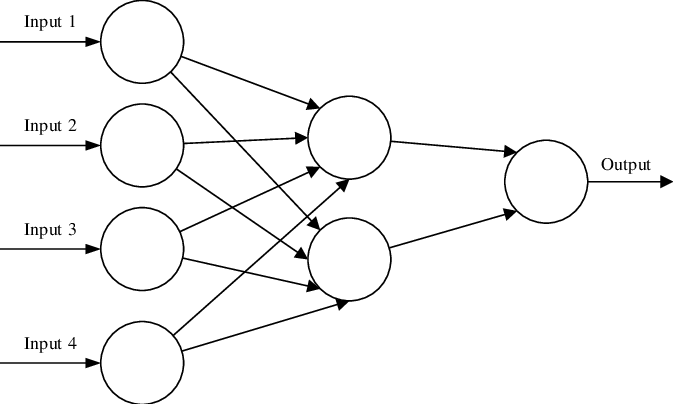
\includegraphics[scale=.25]{nn_intro} 
	\end{minipage} \vspace*{3mm} \\~\\
	To store an image, your computer stores three different matrices corresponding to the red, green, and blue channel (RGB values). So if your input image is 64x64 pixels, you will have three 64x64 matrices. To unroll these values into a \textbf{feature vector}, we will add values from all 3 vectors into a single x vector, where $n_x$ is the number of features in the vector (in this case, 12288). \vspace*{2mm} \\
	In \textbf{binary classification}, our goal is to learn a classifier that can input an image represented by feature vector \textit{x} and predict whether the corresponding label y is a 1 or 0 (1 for cat, 0 for non cat). \vspace*{2mm} \\
	Here is some common notation we will be using: \vspace*{1mm} \\
	\hspace*{3mm} - Single training example: (x,y) where $x \in \mathbb{R}^{n_x}$, y $\in \{0,1\} $ \vspace*{1mm} \\
	\hspace*{3mm} - M training examples: $\{(x^1, y^1), ..., (x^m, y^m)\}$  \vspace*{1mm} \\
	\hspace*{3mm} - Matrix X: $\begin{bmatrix} | & | & ... & | \\ x^1 & x^2 & ... & x^m \\ | & | & ... & | \end{bmatrix}$ where rows = $n_x$, columns = m. In Python, X.shape = ($n_x$, m). \vspace*{2mm} \\
	\hspace*{3mm} - Matrix Y: $\begin{bmatrix} y^1, y^2, ..., y^m \end{bmatrix}$ where Y.shape = (1, m) \\~\\
	Given x, we want an estimate known as $\hat{y}$ = P(y=1$|$x) given the following parameters: $x \in \mathbb{R}^{n_x}$, $w \in \mathbb{R}^{n_x}$, and $b \in \mathbb{R}$. We want out output to be $0 \leq \hat{y} \leq 1$, so we will use the \textbf{sigmoid function} to find our output, which will be: $$ \hat{y} = \sigma (z) \;\; \text{where}\;\; z = w^Tx + b \;\; \text{and}\;\; \sigma(z) = \frac{1}{1+e^{-z}}$$ If z is large, then $\sigma(z)$ will be very close to 1. But if z is a large negative number, then $\sigma(z)$ will be very close to 0. So given $\{(x^1, y^1),...,(x^m,y^m)\}$ we want $\hat{y}^i \approx y^i$
	\subsubsection{Logistic Regression Cost Function}
	We will associate $x^i$, $y^i$, and $z^i$ with the $i^{th}$ training example of our data. We will need to define a \textbf{loss function}, with respect to a single training example, to measure how good our output ($\hat{y}$) is when the true label is y. Since we are using gradient descent, we will define the following loss function: $$ \mathcal{L}(\hat{y},y) \; = \; -(y\,log(\hat{y}) \; + \; (1-y)\,log(1-\hat{y}))  $$ We want this loss function to be as small as possible. Lets look at the two cases: \vspace*{1mm} \\
	\hspace*{2mm} If y=1: $ \mathcal{L}(\hat{y},y) \, = \, -y\,log(\hat{y})$ and we want this to be as small as possible ($\hat{y}$ large). \\
	\hspace*{2mm} If y=0: $ \mathcal{L}(\hat{y},y) \, = \, -\,log(1-\hat{y})$ and we want this to be large ($\hat{y}$ small). \newpage
%%%% PAGE 2 %%%%

	\noindent To train the parameters \textit{w} and \textit{b}, we need to define a \textbf{cost function}, which measures how well your doing on an entire training set (cost of the parameters). We will define this as: \\ $$ J(w,b)\, = \, \frac{1}{m}\, \sum_{i=1}^{m}\, \mathcal{L}(\hat{y}^i,y^i) \; = \; -\frac{1}{m}\, \sum_{i=1}^{m}\, [(y^i\,log(\hat{y}^i) \; + \; (1-y^i)\,log(1-\hat{y}^i))] $$
	\subsubsection{Gradient Descent}
	\begin{minipage}[c]{10cm}
	We want to find the values of w and b that will \textit{minimize} the cost function J(w,b). Our cost function that we defined is convex (only one minimum). So we will initialize (w,b) to a random value, typically zero, and will take steps downhill in the steepest direction it can. Eventually it will converge to a minimum value and find our parameter values.
	\end{minipage}
	\begin{minipage}[c]{6cm}
	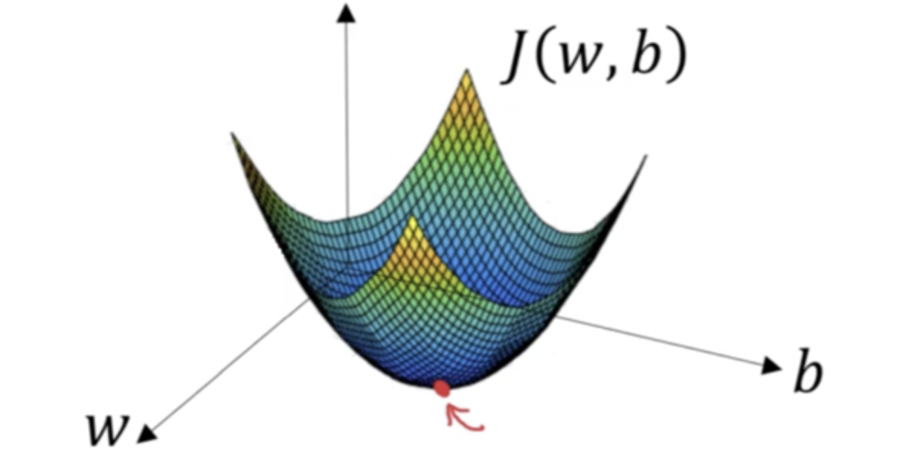
\includegraphics[scale=.4]{grad_desc}
	\end{minipage} \vspace*{4mm} \\~\\
	\textbf{Gradient descent} will repeatedly update the value of w and b with the formula: $$ w \, = \, w \, - \, \alpha \, \frac{ \partial J(w,b)}{\partial w} \; , \; b \, = \, b \, - \, \alpha \, \frac{\partial J(w,b)}{\partial b} $$ where $\alpha$ is our learning rate that we set multiplied by the partial derivative (since there are two variables) of the cost function with respect to the given parameter. \vspace*{2mm} \\
	We want to modify out \textit{w} and \textit{b} parameters in order to reduce the loss when performing gradient descent on our Logistic Regression. We can set up a computation graph to find the derivatives through \textbf{backpropagation}. We will do this for a \textit{single} training example, lets remind ourselves of our equations and the graph: \\
	\begin{minipage}[c]{8cm}
	$ z = w^Tx+ b$ \\
	$\hat{y} = a = \sigma(z)$ \\
	$\mathcal{L}(a,y) \; = \; -(y\,log(a) \; + \; (1-y)\,log(1-a))$ \\
	\end{minipage}
	\begin{minipage}[c]{6cm}
	\vspace*{2mm}
	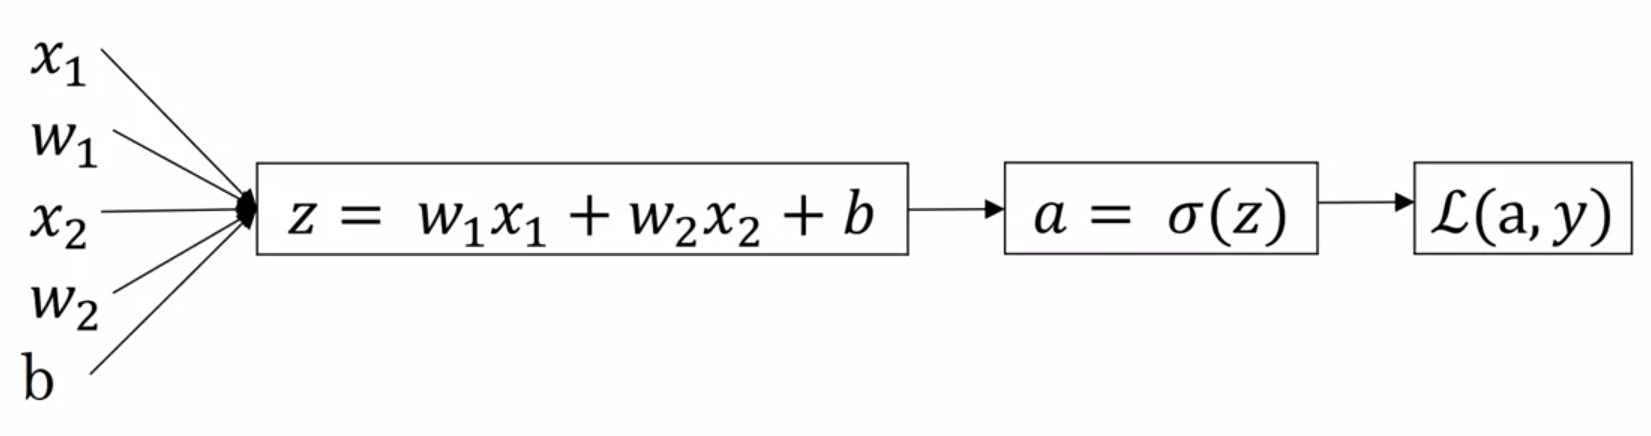
\includegraphics[scale=.2]{comp_graph}
	\end{minipage} \vspace*{1mm} \\~\\
	The first back step is to compute ``da'' = $\frac{\partial \mathcal{L}(a,y)}{\partial a}\; = \; \frac{-y}{a} - \frac{1-y}{1-a}$ \vspace*{2mm}\\
	Next we step back again and compute ``dz'' = $\frac{\partial \mathcal{L}(a,y)}{\partial z}\; = \; \frac{\partial \mathcal{L}}{\partial a}*\frac{\partial a}{\partial z}\; = \; a(1-a)*(\frac{-y}{a} + \frac{1-y}{1-a})\; = \; a-y$ \vspace*{2mm}\\
	The final step back is to find how much to change our $w_1$, $w_2$, and $b$ values. We can do this by: \vspace*{1mm} \\
	\hspace*{2mm} - Calculating: $\frac{\partial \mathcal{L}}{\partial w_1}\;$ = ``$dw_1$" = $x_1 * dz$, ``$dw_2$" = $x_2 * dz$, and ``$db$" = $dz$ \vspace*{1mm} \\
	\hspace*{2mm} - Then update our variables: $w_1 \; = \; w_1 - \alpha* dw_1$, $w_2 \; = \; w_2 - \alpha* dw_2$, and $b \; = \; b - \alpha* dz$ \\~\\
	Now we want to \textbf{perform gradient descent on m examples}. This will use the cost function (not the loss function like we did on a single example). We will write sudo-code for Python that implements this m example gradient descent (assume that $n_x$ = 2): \\
	\begin{minipage}[c]{8cm}
	Initialize: J=0, $dw_1$=0, $dw_2$=0, db=0 \\
	for i=1 to m: \\
	\hspace*{2mm} $z^i = w^Tx^i+b$\\
	\hspace*{2mm} $z^i = \sigma(z^i)$\\
	\hspace*{2mm} $J+= -[(y^i\,log(a^i) \; + \; (1-y^i)\,log(1-a^i))]$\\
	\hspace*{2mm} $dz^i = a^i - y^i$\\
	\hspace*{2mm} $dw_1 += x_1^i*dz^i$\\
	\hspace*{2mm} $dw_2 += x_2^i*dz^i$\\
	\hspace*{2mm} $db += dz^i$
	\end{minipage}
	\begin{minipage}[c]{8cm}
	\vspace*{2mm}
	After the loop, we then take the average and update our varaibles: \vspace*{1mm} \\
	J /= m \\
	$dw_1$ /= m \\
	$dw_2$ /= m \\
	db /= m \vspace*{1mm} \\
	$w_1 \; = \; w_1 - \alpha* dw_1$ \\
	$w_2 \; = \; w_2 - \alpha* dw_2$\\
	 $b \; = \; b - \alpha* db$
	\end{minipage} \newpage
%%%% PAGE 3 %%%%

	\subsubsection{Vectorizing Logistic Regression}
	We often find ourselves training on big data sets and we need our code to run as fast as possible. This is where \textbf{vectorization} comes into play. One example is when we want to calculate $ z = w^Tx + b$. We can use \textit{np.dot(w, x) + b} in Python rather than a \textit{for loop} to decrease our run time by a significant amount. The takeaway from this section is that in deep learning, we want to avoid for loops and use vectorized code (such as NumPy methods) to save time when using large data sets. \\~\\
	Recall that we had defined a matrix, X = $\begin{bmatrix} | & | & ... & | \\ x^1 & x^2 & ... & x^m \\ | & | & ... & | \end{bmatrix}$, that contains the training data. \vspace*{1mm}\\ In order to vectorize finding $ z^i = w^Tx^i + b$ for m training examples, we can instead create a vector of these \textit{z} values, denoted by \textit{Z}.  $$ Z\; =\; [z^1,\; z^2,...,\; z^m] = w^TX + [b,\, b,\,...,\,b] = [w^tx^1+b,\; w^tx^2+b,\;...,\; w^tx^m+b]$$ 
	We will also want to vectorize our sigmoid function, which we will see in our programming assignment where we find A = [$a^1, a^2,..., a^m$] = $\sigma(z)$. These are the forward propagations. \\~\\
	Next we will want to vectorize the remaining steps in order to speed up our code. Lets begin with $dz^i = a^i - y^i$. Instead of looping through each training example, we can use vectors we already created, A = [$a^1, a^2,..., a^m$]  and Y = [$y^1, y^2,..., y^m$] . We can define: $$ dZ = A - Y = [a^1-y^1, a^2-y^2,..., a^m-y^m] = [dz^1, dz^2, ..., dz^m] $$ Now we want to vectorize dw for all training examples. We know that $dw^i += x^i_m*dz^i$ must be updated fo each example and then divided by the total number of examples (m), so we define this as: $$ dw = \frac{1}{m}\,X\, dz^T = \frac{1}{m}\, \begin{bmatrix} | & | & ... & | \\ x^1 & x^2 & ... & x^m \\ | & | & ... & | \end{bmatrix} \begin{bmatrix} dz^1\\ | \\ dz^m \end{bmatrix}  = \frac{1}{m}\, [x^1dz^1 + ... + x^m dz^m]$$ Finally, we see $db$ is the sum of $dz^i$ divided by the total number of examples (m), we can write this as: $$ db \, = \, \frac{1}{m} \sum_{i=1}^m dz^i = np.sum(dZ)$$
	Note that the below steps are only one step of gradient descent, you would still need a for loop to perform multiple steps. The new vectorized gradient descent can now be written as: \\
	$$ Z = w^TX+b$$ 
	$$ A = \sigma(z)$$ 
	$$ dZ = A-Y$$ 
	$$ dw = \frac{1}{m}\,X\,dz^t$$ 
	$$ db = \frac{1}{m}\ np.sum(dZ)$$ 
	$$w = w - \alpha dw$$
	$$b = b - \alpha db$$ \newpage
%%%% PAGE 4 %%%%

	\noindent Some quick notes on \textbf{broadcasting} in Python: \vspace*{1mm} \\
	\hspace*{2mm} - When computing a mathematical operation on an (m,n) matrix with either a (1,n) or (m,1) vector, \hspace*{5mm} Python with automatically manipulate it to convert it into an (m,n) matrix to match. \vspace*{1mm} \\
	\hspace*{2mm} - When computing a mathematical operation on a row vector (m,1) with a real number, Python will \hspace*{5mm} copy the number m times in order to match the sizes of the two vectors. \vspace*{1mm} \\
	\hspace*{2mm} - To simplify your code, don't use ``rank 1" arrays (m,). Instead use either column vectors (m,1) or \hspace*{5mm} row vectors (1,m) to avoid any errors. You can use assert statements to ensure they are the correct \hspace*{5mm} dimensions and reshape() to change any dimensions needed. \\~\\
	Lets take an in depth look at the math behind the \textbf{Logistic Regression cost function}: \vspace*{1mm} \\
	Remember that $\hat{y} = \sigma(w^Tx+b)$ where $\sigma(z) = \frac{1}{1+e^{-z}}$. We interpret $\hat{y} = P(y=1\,|\,x)$ such that: \\
	\hspace*{3mm} If y=1 : P(y$|$x) = $\hat{y}$ \\
	\hspace*{3mm} If y=0 : P(y$|$x) = 1-$\hat{y}$ \vspace*{1mm}\\
	We know that P(y$|$x) = $\hat{y}^y*(1-\hat{y})^{(1-y)}$ and by taking the log of this, we get: $$ log(p(y|x))\; = \; log(\hat{y}^y*(1-\hat{y})^{(1-y)})$$ $$ log(p(y|x))\; = \; ylog(\hat{y})+ (1-y)log(1-\hat{y})$$ 
	We know that the above equation for log(p(y$|$x)) can be denoted as -$\mathcal{L}(\hat{y},y)$, which is our cost function. This is only for one example, but we need to find this for \textit{m} examples. We will use \textbf{maximum likelihood estimation} to find the parameters that maximize this equation: $$ log(p(m\; examples))\; = \; log(\prod_{i=1}^{n} p(y^i|x^i)) $$ $$ log(p(m\; examples))\; = \; \sum_{i=1}^m log(p(y^i|x^i)) $$ $$ log(p(m\; examples))\; = \; -\sum_{i=1}^m \mathcal{L}(\hat{y}^i,y^i) $$ This justifies out cost function, and because now we want to minimize the cost we drop the negative sign and to make sure our quantities are scaled, we add the $\frac{1}{m}$. Note that minimizing the loss below corresponds to maximizing log(p(y$|$x)).  $$ J(w,b) = \frac{1}{m} \sum_{i=1}^{m} \mathcal{L}(\hat{y}^i,y^i) = \frac{1}{m}\, \sum_{i=1}^{m}\, [(y^i\,log(\hat{y}^i) \; + \; (1-y^i)\,log(1-\hat{y}^i))] $$
	\subsubsection{Programming Assignment}
	Problem Statement: You are given a dataset ("data.h5") containing: \\
	\hspace*{3mm} - A training set of m\_train images labeled as cat (y=1) or non-cat (y=0). \\
	\hspace*{3mm} - A test set of m\_test images labeled as cat or non-cat. \\
	\hspace*{3mm} - Each image is of shape (num\_px, num\_px, 3) where 3 is for the 3 channels (RGB). Thus, each image \hspace*{6mm} is square (height = num\_px) and (width = num\_px). \vspace*{1mm} \\
	You will build a simple image-recognition algorithm that can correctly classify pictures as cat or non-cat. We added "\_orig" at the end of image datasets (train and test) because we are going to preprocess them. After preprocessing, we will end up with train\_set\_x and test\_set\_x. 
	\begin{lstlisting}
	# Loading the data (cat/non-cat)
	train_set_x_orig, train_set_y, test_set_x_orig, test_set_y, classes = load_dataset() \end{lstlisting} \newpage
%%%% PAGE 5 %%%%

	\noindent Lets find the dimensions of our data. Remember that train\_set\_x\_orig is a NumPy-array of shape (m\_train, num\_px, num\_px, 3). 
	\begin{lstlisting}
	m_train = train_set_x_orig.shape[0] # 209 examples
	m_test = test_set_x_orig.shape[0] # 50 examples
	num_px = train_set_x_orig.shape[1] # 64 \end{lstlisting} \vspace*{1mm} 
	Note that each image is of size (64, 64, 3), the training set has shape (209, 64, 64, 3) with corresponding labels (1, 209), and the test set has shape (50, 64, 64, 3) with corresponding labels (1,50). \vspace*{2mm} \\
	We now want to reshape the training and test data sets so that images of size (num\_px, num\_px, 3) are \textbf{flattened} into single vectors of shape (num\_px*num\_px*3, 1). To flatten a matrix X of shape (a,b,c,d) to a matrix X\_flatten of shape (b*c*d, a) we use: X\_flatten = X.reshape(X.shape[0], -1).T
	\begin{lstlisting}
	train_set_x_flatten = train_set_x_orig.reshape(train_set_x_orig.shape[0], -1).T
	test_set_x_flatten = test_set_x_orig.reshape(test_set_x_orig.shape[0], -1).T 
	
	train_set_x_flatten.shape # (12288, 209)
	test_set_x_flatten.shape # (1288, 50) \end{lstlisting} \vspace*{1mm} 
	Now we will \textbf{standardize} our dataset. One common practice is to subtract the mean of the whole NumPy array from each example, and then divide each example by the standard deviation. But for picture datasets, it is simpler and more convenient and works almost as well to just divide every row of the dataset by 255 (since the range for the vector values of an image are [0, 255]). 
	\begin{lstlisting}
	train_set_x = train_set_x_flatten/255.
	test_set_x = test_set_x_flatten/255. \end{lstlisting} \vspace*{1mm} 
	\hspace*{16mm} 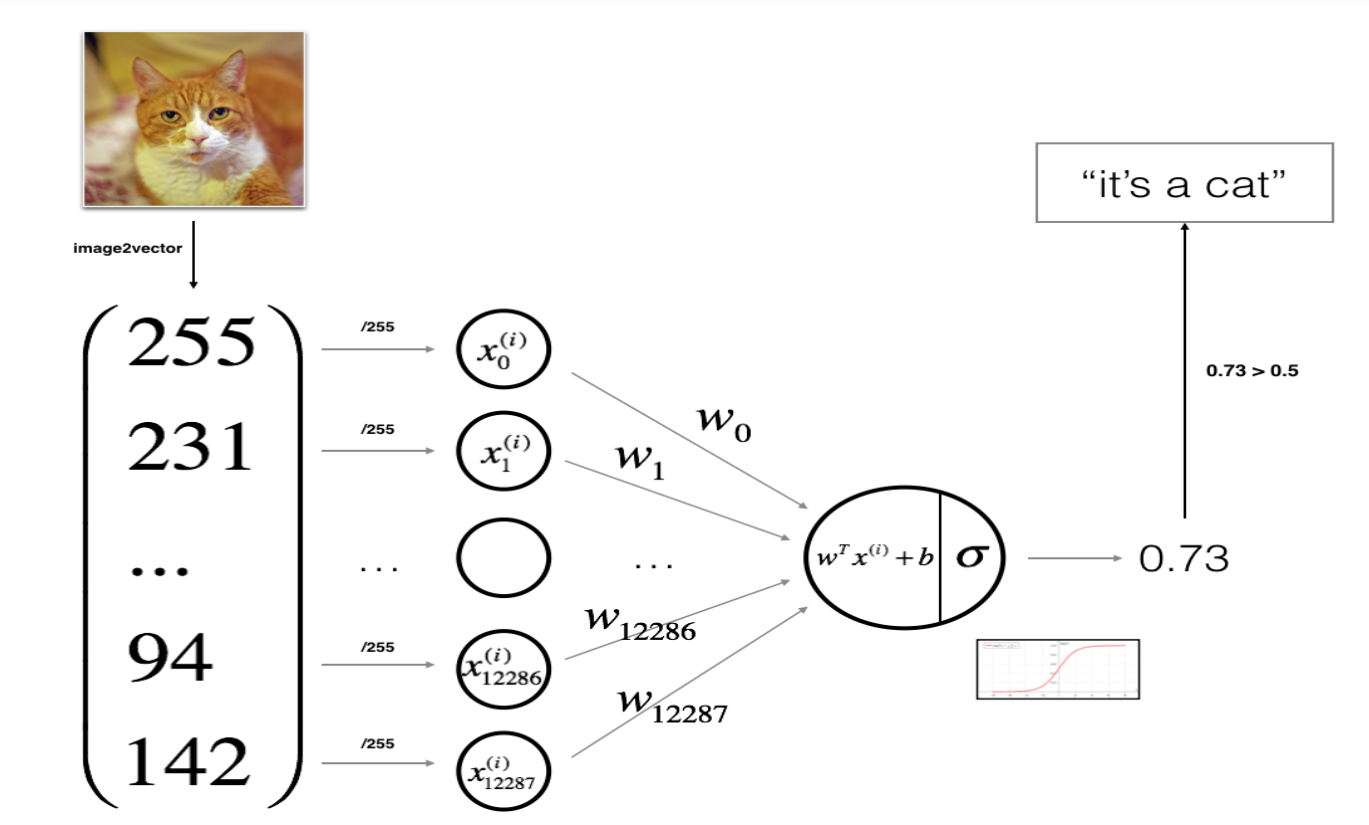
\includegraphics[scale=.5]{cat_log} \\
	Above is a depiction of how our Logistic Regression Neural Network will operate (refer to the previous section for an explanation of the mathematical expressions). We will carry out the following steps: \\
	\hspace*{3mm} - Initialize the parameters of the model. \\
	\hspace*{3mm} - Learn the parameters for the model by minimizing the cost. \\
	\hspace*{3mm} - Use the learned parameters to make predictions (on the test set). \\
	\hspace*{3mm} - Analyze the results and conclude. \vspace*{2mm} \\
	Lets begin building the parts of our algorithm. There are 3 main steps for \textbf{building a Neural Network}: \\
	\hspace*{3mm} 1. Define the model structure (such as number of input features). \\
	\hspace*{3mm} 2. Initialize the model's parameters. \\
	\hspace*{3mm} 3. Loop: \\
	\hspace*{7mm} - Calculate current loss (forward propagation). \\
	\hspace*{7mm} - Calculate current gradient (backward propagation). \\
	\hspace*{7mm} - Update parameters (gradient descent). \newpage
%%%% PAGE 6 %%%%

	\begin{lstlisting}
	def sigmoid(z):
		# Compute sigmoid of z = w.T * x + b
		s = 1 / (1+np.exp(-z))
		return s
	
	def initialize_with_zeros(dim):
		# Creates a vector of zeros of shape (dim, 1) for w and initializes b=0.
		w = np.zeros((dim,1))
		b = 0
		return w, b \end{lstlisting} \vspace*{1mm} 
	Now that your parameters are initialized, you can do the \textbf{forward/backward propagation} steps for learning the parameters. The steps for forward propagation are: \vspace*{1mm} \\
	\hspace*{3mm} - You get X \\
	\hspace*{3mm} - You compute $A = \sigma(w^T X + b) = (a^{1}, a^{2}, ..., a^{m-1}, a^{m})$ \\
	\hspace*{3mm} - You calculate the cost function: $J = -\frac{1}{m}\sum_{i=1}^{m}y^{i}\log(a^{i})+(1-y^{i})\log(1-a^{i})$  \vspace*{2mm} \\
	The steps for back propagation are: \vspace*{1mm} \\
	\hspace*{3mm} - Compute $ \frac{\partial J}{\partial w} = \frac{1}{m}X(A-Y)^T$ \vspace*{1mm}\\
	\hspace*{3mm} - Compute $ \frac{\partial J}{\partial b} = \frac{1}{m} \sum_{i=1}^m (a^{i}-y^{i})$
	\begin{lstlisting}
	def propagate(w, b, X, Y):
		"""
		Implement the cost function and its gradient for the propagation explained above
		Arguments:
		w -- weights, a numpy array of size (num_px * num_px * 3, 1)
		b -- bias, a scalar
		X -- data of size (num_px * num_px * 3, number of examples)
		Y -- true "label" vector (containing 0 if non-cat, 1 if cat) of size (1, m)
		
		Return:
		cost -- negative log-likelihood cost for logistic regression
		dw -- gradient of the loss with respect to w, thus same shape as w
		db -- gradient of the loss with respect to b, thus same shape as b
		"""
		
		m = X.shape[1]
		
		# FORWARD PROPAGATION (FROM X TO COST)
		A = sigmoid(np.dot(w.T, X) + b) # compute activation
		cost = -(1/m)*np.sum(Y*np.log(A) + (1-Y)*np.log(1-A)) # compute cost
		
		# BACKWARD PROPAGATION (TO FIND GRAD)
		dw = (1/m) * np.dot(X, (A-Y).T)
		db = (1/m) * np.sum(A-Y)
		
		cost = np.squeeze(cost)
		grads = {"dw": dw,
		         "db": db}
		
		return grads, cost \end{lstlisting} \vspace*{1mm} 
	Now that we have initialized our parameters and can compute a cost function and its gradient, we can create an  \textbf{optimize function} to update the parameters using gradient descent. The goal is to learn \textit{w}  and \textit{b} by minimizing the cost function J . For a parameter $\theta$ , the update rule is $\theta = \theta - \alpha d\theta$ , where $\alpha$  is the learning rate. \vspace*{1mm} \\
	We can also create a \textbf{predict} function with our learned parameters to make predictions for a dataset X. We will calculate $\hat{Y}$ = A, and then convert entries to 0 or 1 based on probabilities. \newpage
%%%% PAGE 6 %%%%

	\begin{lstlisting}
	def optimize(w, b, X, Y, num_iterations, learning_rate, print_cost = False):
		"""
		Arguments:
		w -- weights, a numpy array of size (num_px * num_px * 3, 1)
		b -- bias, a scalar
		X -- data of shape (num_px * num_px * 3, number of examples)
		Y -- true "label" vector (containing 0 if non-cat, 1 if cat), of shape (1, m)
		num_iterations -- number of iterations of the optimization loop
		learning_rate -- learning rate of the gradient descent update rule
		print_cost -- True to print the loss every 100 steps
		
		Returns:
		params - dictionary containing the weights w and bias b
		grads - the gradients of the weights and bias with respect to the cost function
		costs - list of all the costs computed during the optimization (graphing)
		"""
		costs = []
		
		for i in range(num_iterations):
			grads, cost = propagate(w, b, X, Y)
			
			dw = grads["dw"] # Retrieve derivatives from grads
			db = grads["db"] # Retrieve derivatives from grads
			
			w = w - learning_rate * dw # update rule
			b = b - learning_rate * db # update rule
			
			if i % 100 == 0: # Record the costs
				costs.append(cost)
			
			if print_cost and i % 100 == 0: # Print the cost every 100 training iterations
				print ("Cost after iteration %i: %f" %(i, cost))
		
		params = {"w": w, "b": b}
		grads = {"dw": dw, "db": db}
		return params, grads, costs
	
	def predict(w, b, X):
	'''
	Predict whether the label is 0 or 1 using learned  parameters (w, b)
	
	Arguments:
	w -- weights, a numpy array of size (num_px * num_px * 3, 1)
	b -- bias, a scalar
	X -- data of size (num_px * num_px * 3, number of examples)
	
	Returns a numpy array (vector) containing all predictions (0/1) for the examples in X
	'''
	m = X.shape[1]
	Y_prediction = np.zeros((1,m))
	w = w.reshape(X.shape[0], 1)
	
	# Compute "A" predicting the probabilities of a cat being present in the picture
	A = sigmoid(np.dot(w.T, X) + b)
	
	for i in range(A.shape[1]): # Convert prob. A[0,i] to actual predictions p[0,i]
		Y_prediction[0,i] = A[0,i] > 0.5 
	
	assert(Y_prediction.shape == (1, m))
	
	return Y_prediction \end{lstlisting} \newpage
%%%% PAGE 8 %%%%

	\noindent The final step is to \textbf{merge all functions into a model} by putting together the previous parts in the correct order. 
	\begin{lstlisting}
	def model(X_train, Y_train, X_test, Y_test, num_iterations = 2000, 
					  learning_rate = 0.5, print_cost = False):
		"""
		Arguments:
		X_train -- training set represented by a np array (num_px * num_px * 3, m_train)
		Y_train -- training labels represented by a np array (1, m_train)
		X_test -- test set represented by a np array (num_px * num_px * 3, m_test)
		Y_test -- test labels represented by a np array (1, m_test)
		num_iterations -- hyperparameter used to optimize the parameters
		learning_rate -- hyperparameter used in the update rule of optimize()
		print_cost -- Set to true to print the cost every 100 iterations
		
		Returns:
		d -- dictionary containing information about the model.
		"""
		w, b = initialize_with_zeros(X_train.shape[0]) # initialize parameters with zeros 
		
		# Gradient descent
		parameters, grads, costs = optimize(w, b, X_train, Y_train, num_iterations, 
										                    learning_rate, print_cost)
		
		# Retrieve parameters w and b from dictionary "parameters"
		w = parameters["w"]
		b = parameters["b"]
		
		Y_prediction_test = predict(w, b, X_test) # Predict test set examples
		Y_prediction_train = predict(w, b, X_train) # Predict test set examples

		# Print train/test Errors
		print("train accuracy: {} %".format(100 - np.mean(np.abs(Y_prediction_train - 
		                                                         Y_train)) * 100))
		print("test accuracy: {} %".format(100 - np.mean(np.abs(Y_prediction_test - 
		                                                        Y_test)) * 100))
		d = {"costs": costs,
		     "Y_prediction_test": Y_prediction_test, 
		     "Y_prediction_train" : Y_prediction_train, 
		     "w" : w, 
		     "b" : b,
		     "learning_rate" : learning_rate,
		     "num_iterations": num_iterations}
		
		return d 
		
	d = model(train_set_x, train_set_y, test_set_x, test_set_y, num_iterations = 2000, 
	          learning_rate = 0.005, print_cost = True) \end{lstlisting} \vspace*{1mm}
	\begin{minipage}[c]{6cm}
	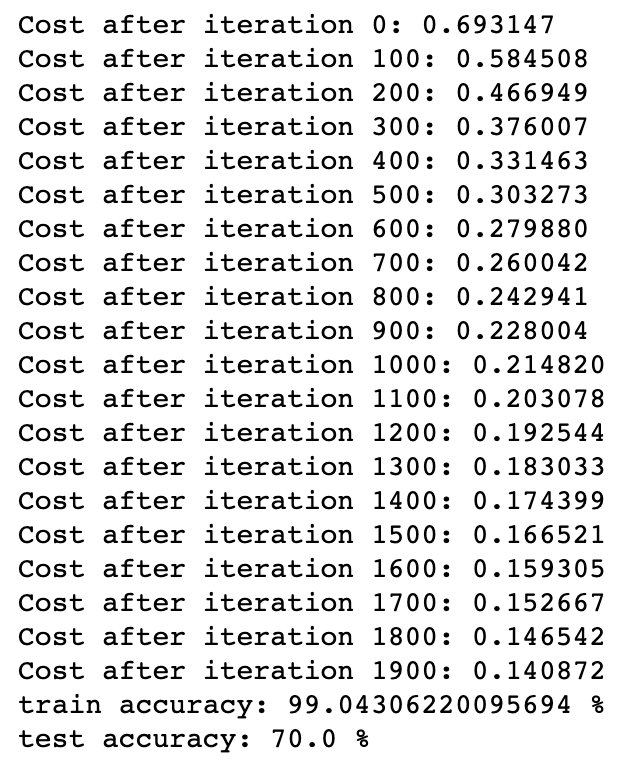
\includegraphics[scale=0.4]{model_output}
	\end{minipage}
	\begin{minipage}[c]{11cm}
	From our model, we can see that the training accuracy is 99\% while the test accuracy is 70\%, which is a cause of overfitting. We can also see that the cost is decreasing per one hundred iterations (meaning the parameters are being leaned). We can continue to decrease the cost by increasing the number of iterations, but this will also cause more overfitting to occur. Given the small dataset and the fact that Logistic Regression is a linear classifier, overall it is not a bad simple model. In the future, we will learn to avoid overfitting and increase the test accuracy.
	\end{minipage} \newpage
%%%% PAGE 9 %%%%

	\subsection{Shallow Neural Network}
	\subsubsection{Overview and Representation}
	Previously, we only had a single sigmoid function in our Logistic Regression model. Now, we will stack multiple sigmoids on top of one another, followed by then feeding these into another sigmoid to create a Neural Network. Some new notation we are introducing: \vspace*{1mm} \\
	\hspace*{3mm} - [\#] will refer to quantities associated with a given layer. \\
	\hspace*{3mm} - (i) will refer to the i$^{th}$ training example (similar to the previous section). \\
	\hspace*{3mm} - a$^{[0]}$ will be the activation layer (same as our vector x that has the input features). \\
	\hspace*{3mm} - a$^{[1]}$ will be the values for our hidden layer. \\
	\hspace*{3mm} - a$^{[2]}$ will be the output layer values (our $\hat{y}$). \\
	\hspace*{3mm} - a$^{[l]}_i$ will be [\textit{l}] = layer, \textit{i} = node in the layer. \vspace*{1mm} \\
	We will be focusing on a \textbf{Two Layer Neural Network}, which has an input layer, one hidden layer, and an output layer. We don't count the input layer as an ``official" layer. The \textit{hidden layer} will have parameters $w^{[1]}$ and $b^{[1]}$, while the output layer has parameters $w^{[2]}$ and $b^{[2]}$ associated with it. 
	\hspace*{16mm} 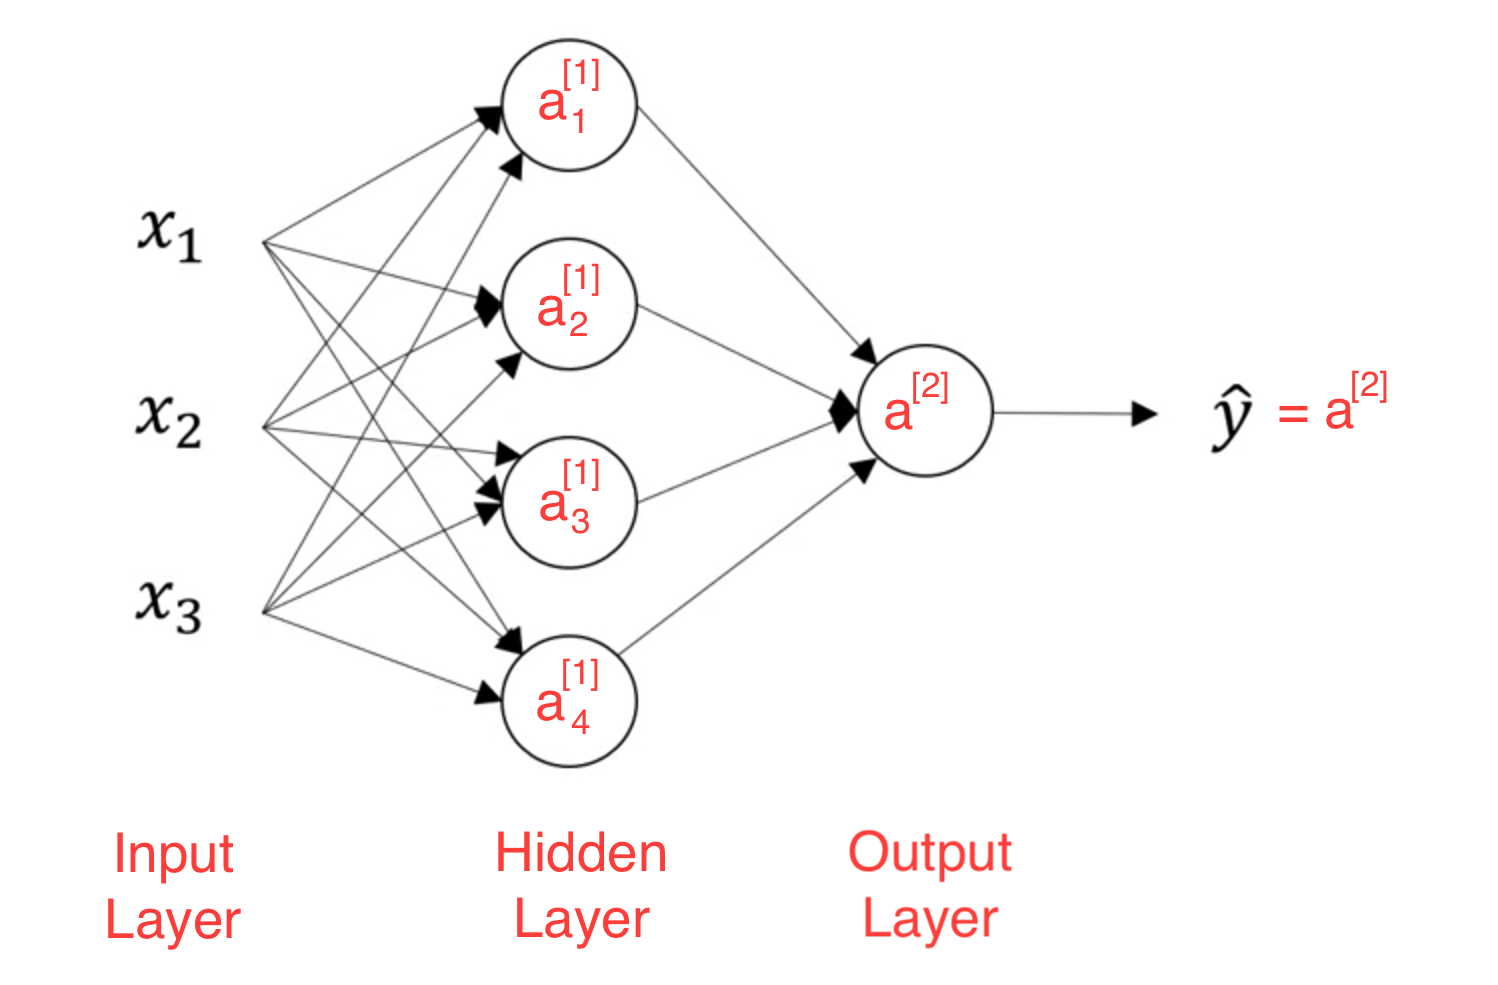
\includegraphics[scale=.5]{NN_rep} 
	\subsubsection{Computing a Neural Network Output}
	\begin{minipage}[c]{9cm}
	Each node in our hidden layer will take all of the input values from x, compute z, and input this value into an activation function (sigmoid). Since each node has to compute z, we will vectorize this process by using matrix multiplication in python. This gives us the following equation to find our vector $z^{[1]}$ and our activation vector $a^{[1]}$ for the hidden layer.
	\end{minipage}
	\begin{minipage}[c]{5cm}
	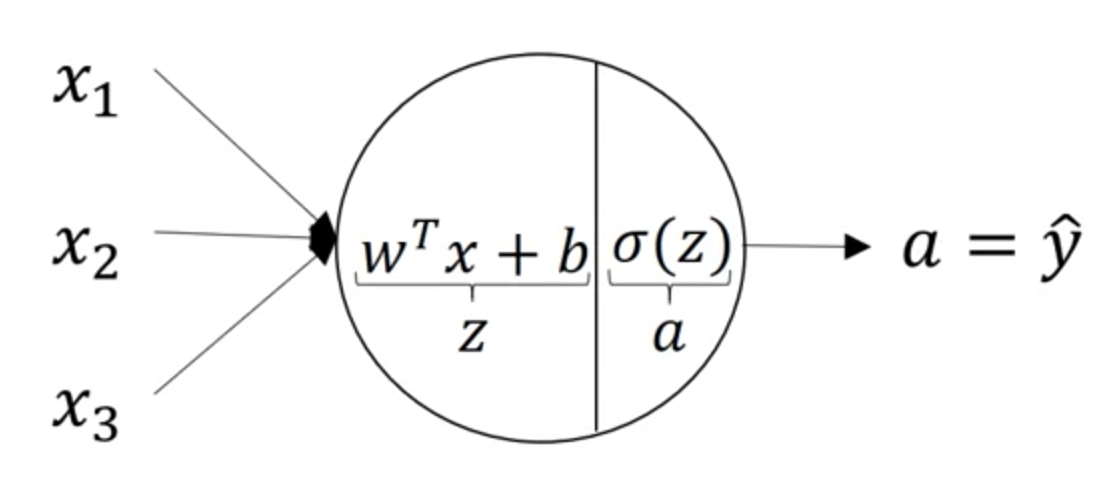
\includegraphics[scale=0.4]{act_func}
	\end{minipage} \vspace*{4mm} \\
	$$ z^{[1]} = \begin{bmatrix} -\, w_1^{[1]T}\, - \vspace*{.5mm} \\ -\, w_2^{[1]T}\, - \vspace*{.5mm} \\ -\, w_3^{[1]T}\, - \vspace*{.5mm} \\ -\, w_4^{[1]T}\, - \vspace*{.5mm} \end{bmatrix} * \begin{bmatrix} x_1 \\ x_2 \\ x_3 \end{bmatrix} + \begin{bmatrix} b_1^{[1]} \vspace*{.5mm}\\ b_2^{[1]} \vspace*{.5mm}\\ b_3^{[1]} \vspace*{.5mm}\\ b_4^{[1]} \vspace*{.5mm}\\  \end{bmatrix} = \begin{bmatrix} w_1^{[1]T}x + b_1^{[1]} \vspace*{.5mm} \\ w_2^{[1]T}x + b_2^{[1]}  \vspace*{.5mm} \\ w_3^{[1]T}x + b_3^{[1]} \vspace*{.5mm} \\ w_4^{[1]T}x + b_4^{[1]}  \vspace*{.5mm} \end{bmatrix} = \begin{bmatrix} z_1^{[1]} \vspace*{.5mm}\\ z_2^{[1]} \vspace*{.5mm}\\ z_3^{[1]} \vspace*{.5mm}\\ z_4^{[1]} \vspace*{.5mm}\\  \end{bmatrix},\;\; \text{also let}\; a^{[1]} = \begin{bmatrix} a_1^{[1]} \vspace*{.5mm}\\ a_2^{[1]} \vspace*{.5mm}\\ a_3^{[1]} \vspace*{.5mm}\\ a_4^{[1]}  \end{bmatrix} = \sigma(z^{[1]}) $$
	Note: Let the matrix with the \textit{w} values be denoted as $W^{[1]}$ and the vector holding \textit{b} values be $b^{[1]}$. \newpage
%%%% PAGE 10 %%%%

	\noindent For the \textbf{hidden layer}, this gives us the general formulas (remember x = $a^{[0]}$): \vspace*{1mm} \\
	\hspace*{3mm} $z^{[1]} = W^{[1]}a^{[0]} + b^{[1]}$ with shapes: $z^{[1]}=(4,1),\; W^{[1]}=(4,3),\; a^{[0]}=(3,1),\; b^{[1]}=(4,1)$ \vspace*{1mm} \\
	\hspace*{3mm} $a^{[1]} = \sigma(z^{[1]})$ with shapes: $a^{[1]}=(4,1),\; z^{[1]}=(4,1)$ \vspace*{2mm} \\
	For the \textbf{output layer}, this gives us the following formulas (output $a^{[1]}$ used as input ``x"): \vspace*{1mm} \\
	\hspace*{3mm} $z^{[2]} = W^{[2]}a^{[1]} + b^{[2]}$ with shapes: $z^{[2]}=(1,1),\; W^{[2]}=(1,4),\; a^{[1]}=(4,1),\; b^{[2]}=(1,1)$ \vspace*{1mm} \\
	\hspace*{3mm} $a^{[2]} = \sigma(z^{[2]})$ with shapes: $a^{[2]}=(1,1),\; z^{[2]}=(1,1)$
	\subsubsection{Vectorizing Across Multiple Examples}
	When we want to compute predictions for all of our training examples (not just a single example like we did above), we need to vectorize a method in order to compute all of these at once. Some new notation we will use: \vspace*{1mm} \\
	\hspace*{3mm} - ex: a$^{[2](i)}$ refers to the layer 2 value for the i$^{th}$ training example. \vspace*{1mm} \\
	We will define the following matrices to work with $n_x$ training examples where X = m training examples, Z$^{[1]}$ = is all of the z$^{[1]}$ values for m training example, and A$^{[1]}$ = all of our a$^{[1]}$ values for m training examples. Note that the format is the same for Z$^{[2]}$ and A$^{[2]}$ with their corresponding values. $$ X = \begin{bmatrix} | & | & ... & | \\ x^1 & x^2 & ... & x^m \\ | & | & ... & | \end{bmatrix} \hspace*{5mm} Z^{[1]} = \begin{bmatrix} | & | & ... & | \\ z^{[1](1)} & z^{[1](2)}  & ... & z^{[1](m)}  \\ | & | & ... & | \end{bmatrix} \hspace*{5mm} A^{[1]} = \begin{bmatrix} | & | & ... & | \\ a^{[1](1)} & a^{[1](2)}  & ... & a^{[1](m)}  \\ | & | & ... & | \end{bmatrix} $$
	This gives us the following \textbf{vectorized formulas} to find all predicted values for m examples: \vspace*{1mm} \\
	\hspace*{3mm} $Z^{[1]} = W^{[1]}X + b^{[1]}$  \vspace*{1mm} \\
	\hspace*{3mm} $A^{[1]} = \sigma(Z^{[1]})$  \vspace*{1mm} \\
	\hspace*{3mm} $Z^{[2]} = W^{[2]}A^{[1]} + b^{[2]}$  \vspace*{1mm} \\
	\hspace*{3mm} $A^{[2]} = \sigma(Z^{[2]})$ 
	\subsubsection{Activation Functions}
	Previously, we have used the sigmoid function as our activation function. However, there are much better functions that we can use instead, denoted by a general symbol \textit{g}. For a Two Layer Neural Network, we can denote the activation function for the \textbf{hidden layer} as $g^{[1]}(z^{[1]})$ and the \textbf{output layer} as $g^{[2]}(z^{[2]})$. \vspace*{2mm} \\
	One exception is when you are doing binary classification to use a sigmoid function for the output layer. This is because a a sigmoid function will output a value between 0 and 1, which works perfectly since our true labels (y) will either be a 0 or 1. \vspace*{2mm} \\
	Another option for an activation function is tanh(z). This is often much more useful than the sigmoid function, and will output a value in the range [-1,1]. A downfall to both the sigmoid and tanh function are that when z is very large or small, the gradient is near 0 and can cause gradient descent to slow. The most commonly used activation function is the ReLU function (or the Leaky ReLU function to avoid having a 0 gradient for negative numbers). \vspace*{2mm} \\
	\hspace*{24mm} 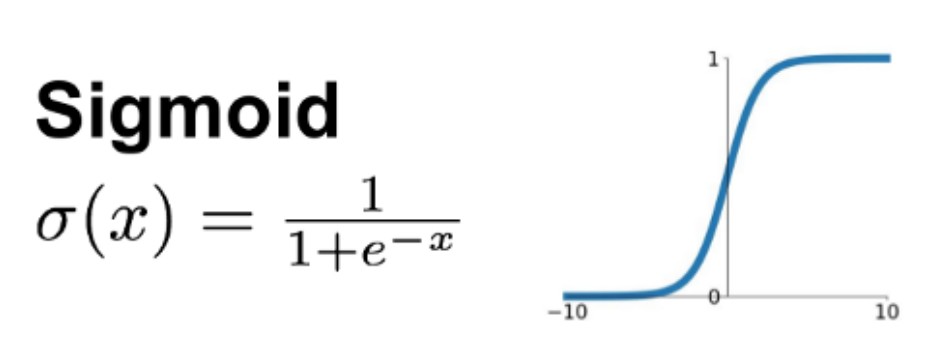
\includegraphics[scale=0.3]{sigmoid} \hspace*{15mm} 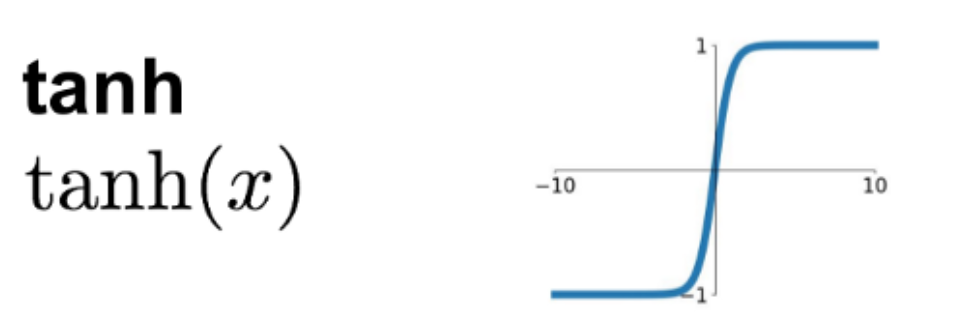
\includegraphics[scale=0.3]{tanh} \\
	\hspace*{24mm} 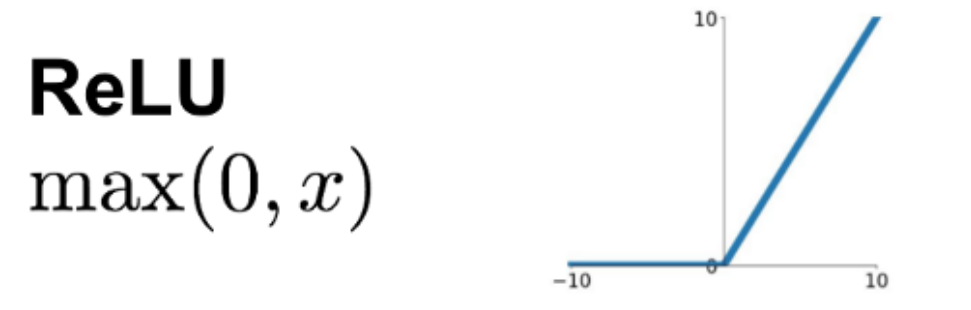
\includegraphics[scale=0.3]{relu} \hspace*{13mm} 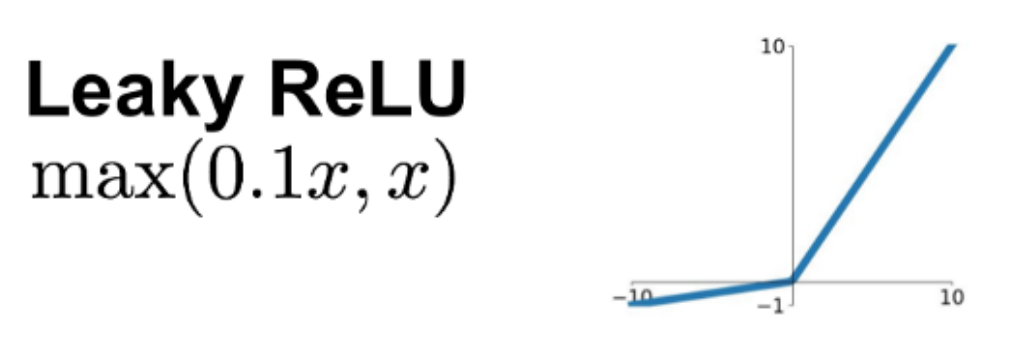
\includegraphics[scale=0.3]{leaky_relu} \newpage
%%%% PAGE 11 %%%%

	\subsubsection{Gradient Descent for Neural Networks}
	A Neural Network with one hidden layer will have the following: \vspace*{1mm} \\
	\hspace*{3mm} - Parameters: $W^{[1]}$ with shape ($n^{[1]},n^{[0]})$.\\ \hspace*{28mm} $b^{[1]}$ with shape $(n^{[1]},1)$.\\ \hspace*{28mm} $W^{[2]}$ with shape $(n^{[2]},n^{[1]})$.\\ \hspace*{28mm} $b^{[2]}$ with shape $(n^{[2]},1)$. \vspace*{1mm} \\
	\hspace*{3mm} - $n^{[0]}$ input features (known as $n_x$), $n^{[1]}$ hidden layer units, and $n^{[2]}$ output units. \vspace*{1mm} \\
	\hspace*{3mm} - Cost Function: J($W^{[1]}$, $b^{[1]}$, $W^{[2]}$, $b^{[2]}$) = $\frac{1}{m} \sum_{i=1}^{m}\mathcal{L}(\hat{y},y)$ \vspace*{1mm} \\
	\hspace*{3mm} - Gradient descent (repeat the following steps): \vspace*{.5mm} \\
	\hspace*{8mm} 1) Compute predicts ($\hat{y}^{(i)}, ..., \hat{y}^{(m)}$) \\
	\hspace*{8mm} 2) Compute $dW^{[1]} = \frac{dJ}{dw^{[1]}}$, $db^{[1]} = \frac{dJ}{db^{[1]}}$, ... and similary for $dW^{[2]}$ and $db^{[2]}$ \vspace*{.5mm} \\
	\hspace*{8mm} 3) Compute $W^{[1]} = W^{[1]} - \alpha\, dw^{[1]}$ \vspace*{.5mm} \\
	\hspace*{8mm} 4) Compute $b^{[1]} = b^{[1]} - \alpha\, db^{[1]}$ \vspace*{.5mm} \\
	\hspace*{8mm} 5) Compute $W^{[2]} = W^{[2]} - \alpha\, dw^{[2]}$ \vspace*{.5mm} \\
	\hspace*{8mm} 6) Compute $b^{[2]} = b^{[2]} - \alpha\, db^{[2]}$ \vspace*{2mm} \\
	Recall the formulas for \textbf{forward propagation} (where \textit{g} is the generalized activation function): \vspace*{.5mm} \\
	\hspace*{3mm} $Z^{[1]} = W^{[1]}X + b^{[1]}$  \vspace*{1mm} \\
	\hspace*{3mm} $A^{[1]} = g^{[1]}(Z^{[1]})$  \vspace*{1mm} \\
	\hspace*{3mm} $Z^{[2]} = W^{[2]}A^{[1]} + b^{[2]}$  \vspace*{1mm} \\
	\hspace*{3mm} $A^{[2]} = g^{[2]}(Z^{[2]})$ \vspace*{2mm} \\
	This means that we can perform \textbf{back propagation} (gradient descent) with the following steps: \vspace*{.5mm} \\
	\hspace*{3mm} $dz^{[2]} = A^{[2]} - Y$ \\
	\hspace*{3mm} $dW^{[2]} = \frac{1}{m}\, dz^{[2]}\,A^{[1]T}$\\
	\hspace*{3mm} $db^{[2]} = \frac{1}{m}\, np.sum(dz^{[2]}, axis=1, keepdims=True)$ \vspace*{.5mm} \\
	\hspace*{3mm} $dz^{[1]} = W^{[2]T}\,dz^{[2]} * g^{[1]'}(Z^{[1]})$, which is an element-wise product of two ($n^{[1]}, m$) matrices. \\
	\hspace*{3mm} $dW^{[1]} = \frac{1}{m}\, dz^{[1]}\,X^{T}$\\
	\hspace*{3mm} $db^{[1]} = \frac{1}{m}\, np.sum(dz^{[1]}, axis=1, keepdims=True)$, which is an ($n^{[1]},1$ vector). \\~\\
	For a Neural Network, we want to \textbf{initialize the weights} to random values instead of zeros (initializing to zero will cause all of the calculations to be symmetric). To randomly initialize our weights: \\ 
	\hspace*{3mm} - Set $W^{[1]}$ = np.random.randn((2,2)) * 0.01 to create small Gaussian random variables.\\ 
	\hspace*{3mm} - Initialize $b^{[1]}$ = np.zero((2,1)) because \textit{b} does not have the symmetry problem that \textit{w} can have. \\
	\hspace*{3mm} - Similarly, we can do the same for $W^{[2]}$ and $b^{[2]}$. 
	\subsubsection{Programming Assignment}
	For this, you will generate red and blue points to form a flower. You will then fit a neural network to correctly classify the points. You will try different layers and see the results. \vspace*{.5mm} \\
	\begin{minipage}[c]{6.5cm}
	\vspace*{1mm} 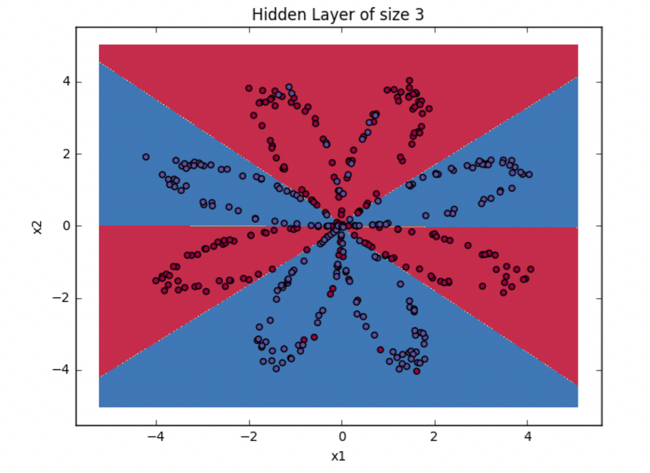
\includegraphics[scale=0.57]{planar} 
	\end{minipage}
	\begin{minipage}[c]{10cm}
	We will learn: \\
	- 2-class classification NN with one hidden layer. \\
	- Use units with a non-linear activation function (ex: tanh). \\
	- Compute the cross entropy loss. \\
	- Implement forward and backward propagation.
	\end{minipage} \newpage
%%%% PAGE 12 %%%%

	\noindent First, lets \textbf{import the packages and dataset} that we will be working with. Also, it will be helpful to visualize the data using matplotlib (notice how it is a flower with two different colored points). For our data, the red corresponds to y=0 and the blue corresponds to y=1. For our data, we have: \\
	\hspace*{3mm} - A NumPy-array (matrix) X that contains your features (x1, x2) \\
	\hspace*{3mm} - A NumPy-array (vector) Y that contains your labels (red:0, blue:1). sc
	\begin{lstlisting}
	import numpy as np
	import matplotlib.pyplot as plt
	from testCases_v2 import * # test examples to test correctness of functions
	import sklearn
	import sklearn.datasets
	import sklearn.linear_model
	from planar_utils import plot_decision_boundary, sigmoid, load_planar_dataset, 
										       load_extra_datasets

	np.random.seed(1) # set a seed so that the results are consistent
	
	X, Y = load_planar_dataset()

	shape_X = X.shape # (2, 400)
	shape_Y = Y.shape # (1, 400)
	m = X.shape[1] # 400 \end{lstlisting}
	We are going to build a Neural Network model with one hidden layer. Lets take a look at the \textbf{setup} for our model and the \textbf{mathematical equations} that correspond to them. Note that we will use the \textit{tanh} activation function for the hidden layer, and the \textit{sigmoid} activation function for the output layer since it is binary classification. \\
	\hspace*{27mm} 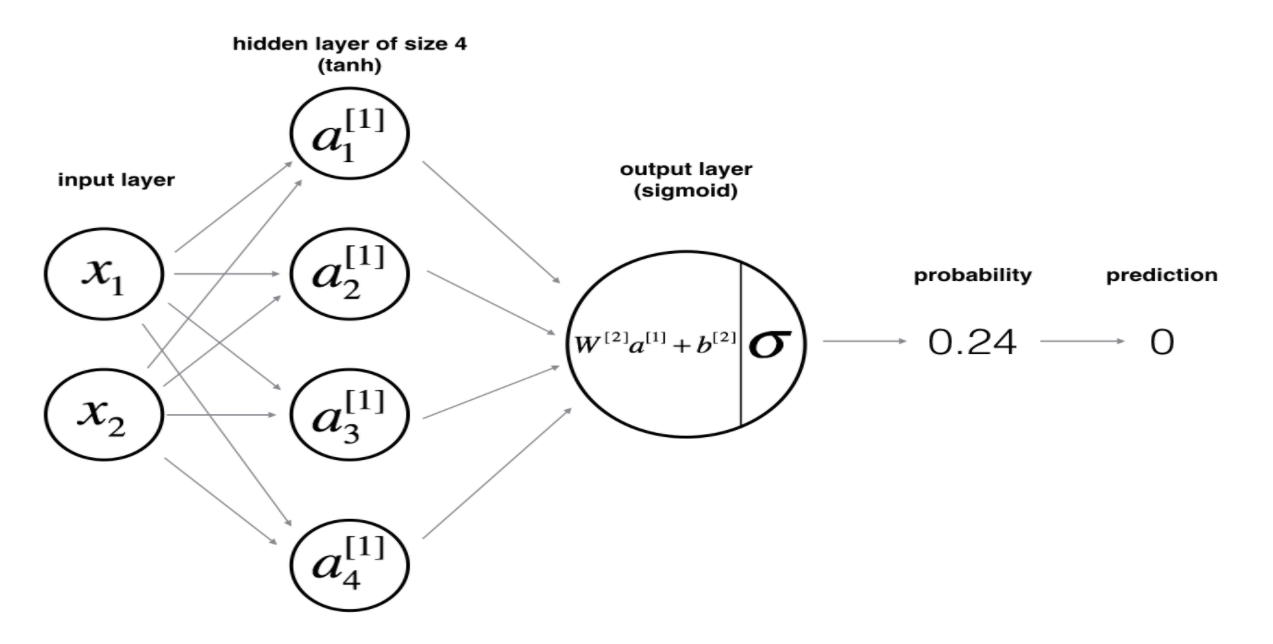
\includegraphics[scale=0.55]{planar_nn} \vspace*{1mm} \\
	For one example $x^{(i)}$: \\
	$$z^{[1] (i)} =  W^{[1]} x^{(i)} + b^{[1]}$$ 
	$$a^{[1] (i)} = \tanh(z^{[1] (i)})$$
	$$z^{[2] (i)} = W^{[2]} a^{[1] (i)} + b^{[2]}$$
	$$\hat{y}^{(i)} = a^{[2] (i)} = \sigma(z^{ [2] (i)})$$
	$$y^{(i)}_{prediction} = \begin{cases} 1 & \mbox{if } a^{[2](i)} > 0.5 \\ 0 & \mbox{otherwise } \end{cases}$$
	\hspace*{4mm} Given the predictions on all the examples, you can also compute the cost $J$ as follows: 
	$$J = - \frac{1}{m} \sum\limits_{i = 0}^{m} \large\left(\small y^{(i)}\log\left(a^{[2] (i)}\right) + (1-y^{(i)})\log\left(1- a^{[2] (i)}\right)  \large  \right) \small$$ \newpage
%%%% PAGE 13 %%%%

	\noindent The \textbf{general methodology} to build a Neural Network is to: \\
	\hspace*{3mm} 1. Define the neural network structure (\# of input units,  \# of hidden units, etc). \\
	\hspace*{3mm} 2. Initialize the model's parameters. \\
	\hspace*{3mm} 3. Loop: \\
	\hspace*{7mm} - Implement forward propagation \\
	\hspace*{7mm} - Compute loss \\
	\hspace*{7mm} - Implement backward propagation to get the gradients \\
	\hspace*{7mm} - Update parameters (gradient descent) \vspace*{1mm} \\
	You often build helper functions to compute steps 1-3 and then merge them into one function we call `nn\_model()`. Once you've built `nn\_model()` and learnt the right parameters, you can make predictions on new data.
	\begin{lstlisting}
	# Step 1: Define the Neural Network structure
	def layer_sizes(X, Y):
		"""
		Arguments:
		X -- input dataset of shape (input size, number of examples)
		Y -- labels of shape (output size, number of examples)
		"""
		n_x = X.shape[0] # size of input layer
		n_h = 4 # size of the hidden layer
		n_y = Y.shape[0] # size of output layer

		return (n_x, n_h, n_y)

	# Step 2: Initialize the model's parameters (random init)
	def initialize_parameters(n_x, n_h, n_y):
		np.random.seed(2) # match example output (but initialization is random). 
		
		W1 = np.random.randn(n_h, n_x) * 0.01 # weight matrix of shape (n_h, n_x)
		b1 = np.zeros((n_h, 1)) # bias vector of shape (n_h, 1)
		W2 = np.random.randn(n_y, n_h) * 0.01 # weight matrix of shape (n_y, n_h)
		b2 = np.zeros((n_y, 1)) # bias vector of shape (n_y, 1)

		parameters = {"W1": W1, "b1": b1, "W2": W2, "b2": b2}
		return parameters 
		
	# Step 3 (part 1): Implement forward propagation
	def forward_propagation(X, parameters):
		"""
		Argument:
		X -- input data of size (n_x, m)
		parameters -- dict containing output of initialization function
		"""
		W1 = parameters['W1']
		b1 = parameters['b1']
		W2 = parameters['W2']
		b2 = parameters['b2']
		
		# Implement Forward Propagation to calculate A2 (probabilities)
		Z1 = np.dot(W1,X) + b1
		A1 = np.tanh(Z1)
		Z2 = np.dot(W2, A1) + b2
		A2 = sigmoid(Z2) # output of second activation function
		
		cache = {"Z1": Z1, "A1": A1, "Z2": Z2, "A2": A2}
		return A2, cache \end{lstlisting} \newpage
%%%% PAGE 14 %%%%

	\noindent Now that you have computed $A^{[2]}$, which contains $a^{[2](i)}$ for every example, you can \textbf{compute the cost} function as follows:
	$$J = - \frac{1}{m} \sum\limits_{i = 1}^{m} \large{(} \small y^{(i)}\log\left(a^{[2] (i)}\right) + (1-y^{(i)})\log\left(1- a^{[2] (i)}\right) \large{)} \small$$
	There's many ways to implement cross-entropy loss. In Python, we implement $- \sum\limits_{i=0}^{m}  y^{(i)}\log(a^{[2](i)})$ as: \\
	logprobs = np.multiply(np.log(A2),Y) \\
	cost = - np.sum(logprobs) \vspace*{2mm} \\
	Note that if you use `np.multiply' followed by `np.sum' the end result will be a type `float', whereas if you use `np.dot', the result will be a 2D NumPy array.  We can use `np.squeeze()' to remove redundant dimensions (in the case of single float, this will be reduced to a zero-dimension array). We can cast the array as a type `float' using `float()'.
	\begin{lstlisting}
	# Step 3 (part 2): Compute the cost
	def compute_cost(A2, Y, parameters):
		"""
		Computes the cross-entropy cost given in equation above
		
		Arguments:
		A2 -- The sigmoid output of the second activation, of shape (1, m)
		Y -- "true" labels vector of shape (1, number of examples)
		parameters -- python dictionary containing your parameters W1, b1, W2 and b2
		"""
		m = Y.shape[1] # number of example
		
		# Compute the cross-entropy cost
		llogprobs = np.multiply(np.log(A2), Y) + np.multiply((1 - Y), np.log(1-A2))
		cost = -(1/m)*np.sum(logprobs)

		cost = float(np.squeeze(cost))  # makes sure cost is the dimension we expect
		return cost \end{lstlisting} \vspace*{1mm}
	Now that we have the cache computed from forward propagation, we can now implement \textbf{backward propagation}. Remember that we will use the six vectorized equations we previously found, which are: \vspace*{1mm} \\
	$$dz^{[2]} = A^{[2]} - Y$$ 
	$$dW^{[2]} = \frac{1}{m}\, dz^{[2]}\,A^{[1]T}$$
	$$db^{[2]} = \frac{1}{m}\, np.sum(dz^{[2]}, axis=1, keepdims=True)$$ 
	$$dz^{[1]} = W^{[2]T}\,dz^{[2]} * g^{[1]'}(Z^{[1]})$$ 
	$$dW^{[1]} = \frac{1}{m}\, dz^{[1]}\,X^{T}$$
	$$db^{[1]} = \frac{1}{m}\, np.sum(dz^{[1]}, axis=1, keepdims=True)$$
	Quick Note: to compute dZ1 you'll need to compute $g^{[1]'}(Z^{[1]})$. Since $g^{[1]}()$ is the tanh activation function, if $a = g^{[1]}(z)$ then $g^{[1]'}(z) = 1-a^2$. So you can compute $g^{[1]'}(Z^{[1]})$ using `(1 - np.power(A1, 2))' in Python. \newpage
%%%% PAGE 15 %%%%

	\begin{lstlisting}
	# Step 3 (part 3): Backward propagation to get gradients
	def backward_propagation(parameters, cache, X, Y):
		"""
		Arguments:
		parameters -- python dictionary containing our parameters 
		cache -- a dictionary containing "Z1", "A1", "Z2" and "A2".
		X -- input data of shape (2, number of examples)
		Y -- "true" labels vector of shape (1, number of examples)
		"""
		m = X.shape[1]

		W1 = parameters['W1']
		W2 = parameters['W2']
		A1 = cache['A1']
		A2 = cache['A2']
		
		# Backward propagation
		dZ2 = A2 - Y
		dW2 = (1/m)*np.dot(dZ2, A1.T)
		db2 = (1/m)*np.sum(dZ2, axis=1, keepdims=True)
		dZ1 = np.dot(W2.T, dZ2) * (1-np.power(A1, 2))
		dW1 = (1/m)*np.dot(dZ1, X.T)
		db1 = (1/m)*np.sum(dZ1, axis=1, keepdims=True)
		
		grads = {"dW1": dW1, "db1": db1, "dW2": dW2, "db2": db2}
		return grads \end{lstlisting}
	Now that we have the gradients, we can implement the \textbf{update rule}. Remember that the general rule is $ \theta = \theta - \alpha \frac{\partial J }{ \partial \theta }$ where $\alpha$ is the learning rate and $\theta$ represents a parameter.
	\begin{lstlisting}
	# Step 3 (part 4): Update parameters using gradient descent
	def update_parameters(parameters, grads, learning_rate = 1.2):
		"""
		Updates parameters using the gradient descent update rule given above
		
		Arguments:
		parameters -- python dictionary containing your parameters 
		grads -- python dictionary containing your gradients 
		"""
		W1 = parameters['W1']
		b1 = parameters['b1']
		W2 = parameters['W2']
		b2 = parameters['b2']

		dW1 = grads['dW1']
		db1 = grads['db1']
		dW2 = grads['dW2']
		db2 = grads['db2']

		# Update rule for each parameter
		W1 = W1 - learning_rate * dW1
		b1 = b1 - learning_rate * db1
		W2 = W2 - learning_rate * dW2
		b2 = b2 - learning_rate * db2
		
		parameters = {"W1": W1, "b1": b1, "W2": W2, "b2": b2}
		return parameters \end{lstlisting}
	Now that we have completed each step in the general methodology to build a Neural Network, we can create a function to put together each of these helper functions. We call this our \textbf{Neural Network Model} function. \newpage
%%%% PAGE 16 %%%%

	\begin{lstlisting}
	def nn_model(X, Y, n_h, num_iterations = 10000, print_cost=False):
		"""
		Arguments:
		X -- dataset of shape (2, number of examples)
		Y -- labels of shape (1, number of examples)
		n_h -- size of the hidden layer
		num_iterations -- Number of iterations in gradient descent loop
		print_cost -- if True, print the cost every 1000 iterations
		
		Returns:
		parameters -- parameters learnt by the model. They can then be used to predict.
		"""
		np.random.seed(3)
		n_x = layer_sizes(X, Y)[0]
		n_y = layer_sizes(X, Y)[2]
		
		# Initialize parameters
		parameters = initialize_parameters(n_x, n_h, n_y)
		
		# Loop (gradient descent)
		for i in range(0, num_iterations):
			# Forward propagation. Outputs: "A2, cache".
			A2, cache = forward_propagation(X, parameters)
			
			# Cost function. Outputs: "cost".
			cost = compute_cost(A2, Y, parameters)
			
			# Backpropagation. Outputs: "grads".
			grads = backward_propagation(parameters, cache, X, Y)
			
			# Gradient descent parameter update. Outputs: "parameters".
			parameters = update_parameters(parameters, grads)
			
			# Print the cost every 1000 iterations
			if print_cost and i % 1000 == 0:
				print ("Cost after iteration %i: %f" %(i, cost))
		
		return parameters \end{lstlisting}
	Now that we can build a complete model, we can make predictions using forward propagation: \vspace*{1mm} \\
	\hspace*{30mm} $y_{prediction} = \text{{activation $>$ 0.5}} = \begin{cases}
	1 & \text{if}\ activation > 0.5 \\
	0 & \text{otherwise}
	\end{cases}$  
	\begin{lstlisting}
	def predict(parameters, X):
		"""
		Using the learned parameters, predicts a class for each example in X
		
		Arguments:
		parameters -- python dictionary containing your parameters 
		X -- input data of size (n_x, m)
		"""
		# Computes probabilities using forward propagation (threshold of 0.5)
		A2, cache = forward_propagation(X, parameters)
		predictions = (A2 > 0.5) # vector of predict 0/1 values
		
		return predictions \end{lstlisting}
	Now that we have a way to create a model and make predictions, we can use this on our planar dataset. We will use a hidden layer of size  4 for our Neural Network. \newpage
%%%% PAGE 17 %%%%

	\begin{lstlisting}
	# Build a model with a n_h-dimensional hidden layer
	parameters = nn_model(X, Y, n_h = 4, num_iterations = 10000, print_cost=True)
	
	# Plot the decision boundary
	plot_decision_boundary(lambda x: predict(parameters, x.T), X, Y)
	plt.title("Decision Boundary for hidden layer size " + str(4)) 
	
	# Print accuracy
	predictions = predict(parameters, X)
	print ('Accuracy: %d' % float((np.dot(Y,predictions.T) + np.dot(1-Y,1-predictions.T))
	                               /float(Y.size)*100) + '%') # 90% \end{lstlisting}
	\begin{minipage}[c]{7.7cm}
	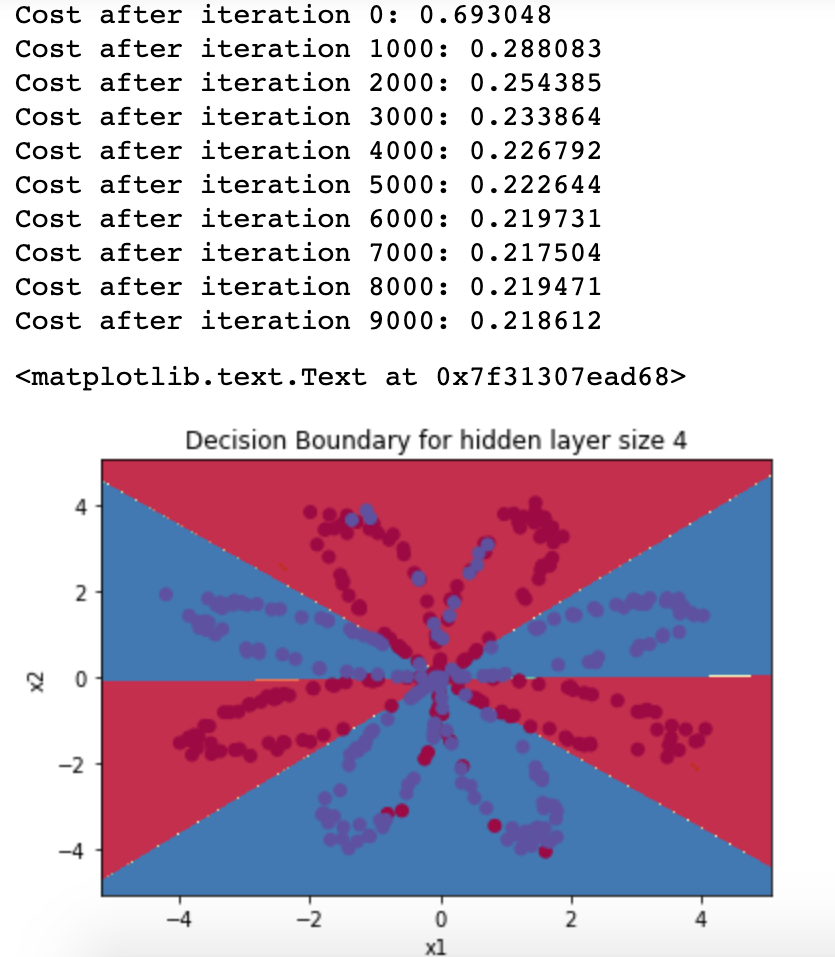
\includegraphics[scale=0.5]{planar_output}
	\end{minipage}
	\begin{minipage}[c]{9.5cm}
	We can see that per 1000 iterations, the cost continued to decrease. The decision boundaries were quite accurate as well. Accuracy is really high (90\%) compared to Logistic Regression. The model has learnt the leaf patterns of the flower! Neural networks are able to learn even highly non-linear decision boundaries, unlike logistic regression. \vspace*{1mm} \\
	If we were to run the Neural Network with many different hidden layer sizes. We can see that around an $n_h$=5 would give us the highest accuracy (around 91\%). The larger models (with more hidden units) are able to fit the training set better, until eventually the largest models overfit the data. We will also learn later about regularization, which lets you use very large models (such as $n_h$ = 50) without much overfitting. 
	\end{minipage} \\~\\
	
	\subsection{Deep L-Layer Neural Network}
	Previously, we have been using a shallow Neural Network with one hidden layer. Now we will focus on a \textbf{deep Neural Network} with multiple hidden layers, with the below exampling being a 4 layer Neural Network with 3 hidden layers. Lets take a look at a diagram and some new notation we will use: \\
	\hspace*{30mm} 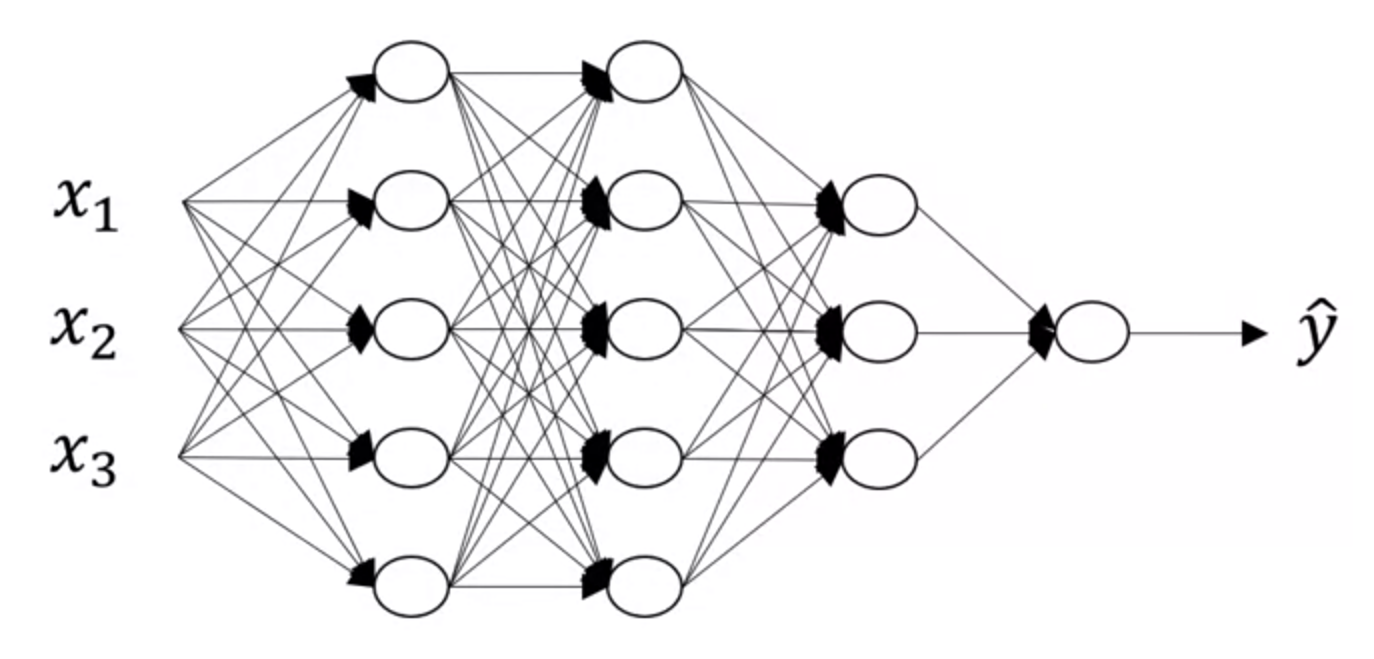
\includegraphics[scale=0.45]{deep_nn} \vspace*{1mm} \\
	L = number of layers in the network. \\
	$n^{[l]}$ = number of units (neurons) in layer \textit{l}. \\
	$a^{[l]}$ = activations in layer \textit{l}, where $a^{[l]} = g^{[l]}(z^[l])$ \\
	$W^{[l]}$ = the weights for corresponding $z^{[l]}$. \\
	$b^{[l]}$ = the corresponding b values for layer \textit{l}. \\
	$a^{[0]}$ = x (the input features for our model). \\
	$a^{[L]}$ = the predicted outputs for our model ($\hat{y}$). \newpage
%%%% PAGE 18 %%%%

	\noindent We will begin with computing forward propagation for a \textbf{single training example} (x). Note that \textit{l} denotes a given layer, \textit{a} represents the input from the previous layer, and \textit{g} is our activation function:
	$$ z^{[l]} = W^{[l]}a^{[l-1]}+b^{[l]}$$ $$ a^{[l]} = g^{[l]}(z^{[l]})$$ 
	Now lets look at the \textbf{vectorized} formulas for computing forward propagation. Remember that the capital letter denotes a matrix that holds all of the values for \textit{m} training examples: 
	$$ Z^{[l]} = W^{[l]}A^{[l-1]}+b^{[l]}$$ $$ A^{[l]} = g^{[l]}(Z^{[l]})$$ 
	Note that for a deep Neural Network, we will have to use a for loop to \textbf{iterate} over \textit{l} = 1, ..., L. Using a for loop for propagation is the only time we are allowed to since there is no other way. \\~\\
	It is very important that our \textbf{matrix dimensions} are correct in order for our outputs to line up with one another. The general shape for each of the variables is as follows: \\~\\
	\begin{minipage}[c]{8cm}
	\hspace*{13mm} For a single training example: $$ z^{[l]} = (n^{[l]},\, 1) $$ $$ W^{[l]} = (n^{[l]},\, n^{[l-1]}) $$ $$ a^{[l]} = (n^{[l-1]},\, 1) $$ $$ b^{[l]} = (n^{[l]},\, 1) $$
	\end{minipage}
	\begin{minipage}[c]{8cm}
	\hspace*{18mm} For \textit{m} training examples: $$ Z^{[l]} = (n^{[l]},\, m) $$ $$ W^{[l]} = (n^{[l]},\, n^{[l-1]}) $$ $$ A^{[l]} = (n^{[l-1]},\, m) $$ $$ b^{[l]} = (n^{[l]},\, 1) $$
	\end{minipage} \\
	\subsubsection{Forward and Backward Propagation}
	We will begin with \textbf{forward propagation} for a layer \textit{l}: \vspace*{1mm} \\
	\hspace*{5mm} Input: $a^{[l-1]}$ \\
	\hspace*{5mm} Output: $a^{[l]}$, cache ($z^{[l]}$)
	$$ Z^{[l]} = W^{[l]}A^{[l-1]}+b^{[l]}$$ $$ A^{[l]} = g^{[l]}(Z^{[l]})$$ 
	Next we want to compute \textbf{backward propagation} for a layer \textit{l}: \vspace*{1mm} \\
	\hspace*{5mm} Input: $da^{[l]}$ \\
	\hspace*{5mm} Output: $da^{[l-1]}, dW^{[l]}, db^{[l]}$
	$$dZ^{[l]} = dA^{[l]}* g^{[l]\prime}(Z^{[l]})$$ $$ dW^{[l]} = \frac{1}{m}\, dZ^{[l]}\, A^{[l-1]T}$$ $$ db^{[l]} = \frac{1}{m}\, np.sum(dZ^{[l]}, axis=1, keepdims=True)$$ $$ dA^{[l-1]} = W^{[l]T}\,dZ^{[l]}$$ 
	We initialize forward propagation with x (our training examples). But for backwards propagation, we initialize with $da^{[l]} = (-\frac{y}{a} + \frac{1-y}{1-a})$ for a single layer \textit{l}. But the vectorized version we initialize with: $$ dA^{[l]} = \begin{bmatrix} (-\frac{y^{(1)}}{a^{(1)}} + \frac{1-y^{(1)}}{1-a^{(1)}}),..., (-\frac{y^{(m)}}{a^{(m)}} + \frac{1-y^{(m)}}{1-a^{(m)}}) \end{bmatrix}  $$ \newpage
%%%% PAGE 19 %%%%

	\noindent A quick note on \textbf{parameters vs. hyperparameters}: \vspace*{1mm} \\
	The parameters for our model are \textit{W} and \textit{b}. The hyperparameters can be things such as learning rate ($\alpha$), number of iterations, number of hidden layers (L), hidden units, activation function, etc. The hyperparameters help to control the final values of \textit{W} and \textit{b}. \vspace*{2mm}\\
	Deep learning is a very empirical process. We may try an idea for a hyperparameter, implement it in our code, and observe the results of the experiment through iterating. It is a trial and error process to find the best hyperparameters for our models. 
	
	\subsubsection{Programming Assignment (Building)}
	For this week, we will build an L-Layer Neural Network. In the next assignment, we will use this model for image classification. Lets begin by importing the necessary packages. 
	\begin{lstlisting}
	import numpy as np
	import h5py
	import matplotlib.pyplot as plt
	from testCases_v4a import *
	from dnn_utils_v2 import sigmoid, sigmoid_backward, relu, relu_backward
	
	%matplotlib inline
	plt.rcParams['figure.figsize'] = (5.0, 4.0) # set default size of plots
	plt.rcParams['image.interpolation'] = 'nearest'
	plt.rcParams['image.cmap'] = 'gray'
	
	%load_ext autoreload
	%autoreload 2
	
	np.random.seed(1) \end{lstlisting}
	To build your neural network, you will be implementing several ``helper functions". These helper functions will be used in the next assignment to build a two-layer and an L-layer neural network. Here is an \textbf{outline of the assignment}: \vspace*{1mm} \\
	\hspace*{3mm} 1) Initialize the parameters for a two-layer network and for an $L$-layer neural network. \\
	\hspace*{3mm} 2) Implement the forward propagation module (shown in purple in the figure below). \\
	\hspace*{7mm} - Complete the LINEAR part of a layer's forward propagation step (resulting in $Z^{[l]}$). \\
	\hspace*{7mm} - We give you the ACTIVATION function (relu/sigmoid). \\
	\hspace*{7mm} - Combine the previous two steps into a new [LINEAR$\rightarrow$ACTIVATION] forward function. \\
	\hspace*{7mm} - Stack the [LINEAR$\rightarrow$RELU] forward function L-1 time (for layers 1 through L-1) and add a \\ \hspace*{9.5mm} [LINEAR$\rightarrow$SIGMOID] at the end (for the final layer $L$). This gives you a new L\_model\_forward \\ \hspace*{9.5mm} function. \\
	\hspace*{3mm} 3) Compute the loss. \\
	\hspace*{3mm} 4) Implement the backward propagation module (denoted in red in the figure below). \\
	\hspace*{7mm} - Complete the LINEAR part of a layer's backward propagation step. \\
	\hspace*{7mm} - We give you the gradient of the ACTIVATE function (relu\_backward/sigmoid\_backward)  \\
	\hspace*{7mm} - Combine the previous two steps into a new [LINEAR$\rightarrow$ACTIVATION] backward function. \\
	\hspace*{7mm} - Stack [LINEAR$\rightarrow$RELU] backward L-1 times and add [LINEAR$\rightarrow$SIGMOID] backward in a new \\ \hspace*{9.5mm} L\_model\_backward function \\
	\hspace*{3mm} 5) Finally update the parameters. \\~\\
	**Note** that for every forward function, there is a corresponding backward function. That is why at every step of your forward module you will be storing some values in a cache. The cached values are useful for computing gradients. In the backpropagation module you will then use the cache to calculate the gradients. \newpage
%%%% PAGE 20 %%%%

	\hspace*{10mm} 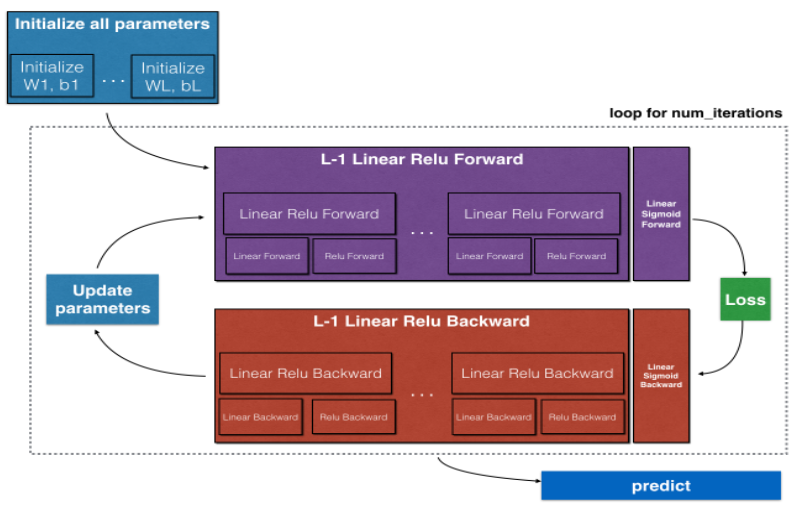
\includegraphics[scale=.65]{deep_fig} \vspace*{1mm} \\
	Lets begin by \textbf{initializing our parameters}. The first function will be for a \textit{two layer model}.
	\begin{lstlisting}
	def initialize_parameters(n_x, n_h, n_y): # Two Layer Neural Network
		"""
		Argument:
		n_x -- size of the input layer
		n_h -- size of the hidden layer
		n_y -- size of the output layer
		"""
		np.random.seed(1)
		
		W1 = np.random.randn(n_h, n_x) * 0.01 # Weight matrix
		b1 = np.zeros((n_h, 1)) # Bias vector
		W2 = np.random.randn(n_y, n_h) * 0.01 # Weight matrix
		b2 = np.zeros((n_y, 1)) # Bias vector
		
		parameters = {"W1": W1, "b1": b1, "W2": W2, "b2": b2}
		return parameters \end{lstlisting}
	The initialization for a \textit{L-layer neural network} is more complicated because there are many more weight matrices and bias vectors. Remember that when we compute $W X + b$ in python, it carries out broadcasting. For example, if: 	
	$$ W = \begin{bmatrix} j  & k  & l\\ m  & n & o \\ p  & q & r \end{bmatrix}\;\;\; X = \begin{bmatrix} a  & b  & c\\	d  & e & f \\
	g  & h & i \end{bmatrix} \;\;\; b =\begin{bmatrix}s  \\ t  \\ u \end{bmatrix}$$
	Then $WX + b$ will be:
	$$ WX + b = \begin{bmatrix} (ja + kd + lg) + s  & (jb + ke + lh) + s  & (jc + kf + li)+ s\\ (ma + nd + og) + t & (mb + ne + oh) + t & (mc + nf + oi) + t\\ (pa + qd + rg) + u & (pb + qe + rh) + u & (pc + qf + ri)+ u \end{bmatrix}  $$
	We will store $n^{[l]}$, the number of units in different layers, in a variable `layer\_dims'. For example, the `layer\_dims' for the ``Planar Data classification model" from last week would have been [2,4,1]: There were two inputs, one hidden layer with 4 hidden units, and an output layer with 1 output unit. This means `W1's shape was (4,2), `b1' was (4,1), `W2' was (1,4) and `b2' was (1,1). Now you will generalize this to $L$ layers. \newpage
%%%% PAGE 21 %%%%

	\begin{lstlisting}
	def initialize_parameters_deep(layer_dims):
	"""
	Arguments:
	layer_dims -- python array containing the dimensions of each layer in our network
	
	Returns:
	parameters -- python dict containing your parameters "W1", "b1", ..., "WL", "bL"
	"""
	np.random.seed(3)
	parameters = {}
	L = len(layer_dims) # number of layers in the network
	
	for l in range(1, L):
		parameters['W' + str(l)] = np.random.randn(layer_dims[l], layer_dims[l-1]) * 0.01
		parameters['b' + str(l)] = np.zeros((layer_dims[l], 1))

	return parameters \end{lstlisting}
	Now that you have initialized your parameters, you will do the \textbf{forward propagation} module. You will start by implementing some basic functions that you will use later when implementing the model: \\
	\hspace*{3mm} 1) LINEAR \\
	\hspace*{3mm} 2) LINEAR $\rightarrow$ ACTIVATION where ACTIVATION will be either ReLU or Sigmoid. \\
	\hspace*{3mm} 3) [LINEAR $\rightarrow$ RELU] $\times$ (L-1) $\rightarrow$ LINEAR $\rightarrow$ SIGMOID (whole model) \vspace*{1mm} \\
	The linear forward module (vectorized over all the examples) computes the following equations: $$Z^{[l]} = W^{[l]}A^{[l-1]} +b^{[l]}$$
	\begin{lstlisting}
	def linear_forward(A, W, b): # Step 1 from above
		"""
		Implement the linear part of a layer's forward propagation.
		"""
		Z = np.dot(W,A) + b # pre-activation parameter (Z = WA + b)
		cache = (A, W, b)
		
		return Z, cache
	
	def linear_activation_forward(A_prev, W, b, activation):  # Step 2 from above
		"""
		Implement the forward propagation for the LINEAR->ACTIVATION layer
		
		Arguments:
		A_prev -- activations from previous layer: (size of previous layer, # of examples)
		W -- weights matrix: shape (size of current layer, size of previous layer)
		b -- bias vector, numpy array of shape (size of the current layer, 1)
		activation -- activation to be used in this layer, stored as: "sigmoid" or "relu"
		"""
		if activation == "sigmoid":
			Z, linear_cache = linear_forward(A_prev, W, b)
			A, activation_cache = sigmoid(Z)
		
		elif activation == "relu":
			Z, linear_cache = linear_forward(A_prev, W, b)
			A, activation_cache = relu(Z)
	
		cache = (linear_cache, activation_cache)
		return A, cache # post-activation value, cache \end{lstlisting} \vspace*{1mm}
	Mathematical relation is: $A^{[l]} = g(Z^{[l]}) = g(W^{[l]}A^{[l-1]} +b^{[l]})$ where the activation ``g" can be sigmoid() or relu(). Note that these are pre-built functions given to us (\href{https://www.kaggle.com/kolisnehar/dnn-utils-v2}{click here for function details}).\newpage
%%%% PAGE 22 %%%%

	\noindent For even more convenience when implementing the $L$-layer Neural Net, you will need a function that replicates the previous one (`linear\_activation\_forwar' with RELU) $L-1$ times, then follows that with one `linear\_activation\_forward' with SIGMOID. \\
	\hspace*{30mm} 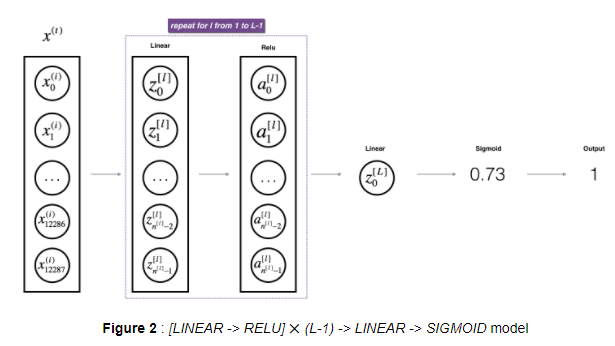
\includegraphics[scale=0.7]{deep_forward_model}
	\begin{lstlisting}
	def L_model_forward(X, parameters):
		"""
		Implement forward propagation for the [LINEAR->RELU]*(L-1)->LINEAR->SIGMOID
		
		Arguments:
		X -- data, numpy array of shape (input size, number of examples)
		parameters -- output of initialize_parameters_deep()
		
		Returns:
		AL -- last post-activation value
		caches -- list of caches containing every cache of linear_activation_forward() 
		          (indexed from 0 to L-1)
		"""
		caches = []
		A = X
		L = len(parameters) // 2 # number of layers in the neural network
		
		# Implement [LINEAR -> RELU]*(L-1). Add "cache" to the "caches" list.
		for l in range(1, L):
			A_prev = A 
			A, cache = linear_activation_forward(A_prev, parameters['W' + str(l)], 
			                                     parameters['b' + str(l)], 'relu')
			caches.append(cache)
		
		# Implement LINEAR -> SIGMOID. Add "cache" to the "caches" list.
		AL, cache = linear_activation_forward(A, parameters['W' + str(L)], 
		                                      parameters['b' + str(L)], 'sigmoid')
		caches.append(cache)
		
		return AL, caches # y-hat (predictions), cache \end{lstlisting} \vspace*{1mm}
	Now we have a full forward propagation that takes the input X and outputs a row vector $A^{[L]}$ containing your predictions. It also records all intermediate values in ``caches". Using $A^{[L]}$, we can now \textbf{compute the cost} of your predictions to check if the model is actually learning. We will compute \textit{Cross-Entropy} cost, \textit{J}, using: $$-\frac{1}{m} \sum\limits_{i = 1}^{m} (y^{(i)}\log\left(a^{[L] (i)}\right) + (1-y^{(i)})\log\left(1- a^{[L](i)}\right))$$ \newpage
%%%% PAGE 23 %%%%

	\begin{lstlisting}
	def compute_cost(AL, Y):
		"""
		Implement the cost function defined by equation (7).
		
		Arguments:
		AL -- probability vector corresponding to your label predictions, shape (1, m)
		Y -- true "label" vector, shape (1, m)
		
		Returns:
		cost -- cross-entropy cost
		"""
		m = Y.shape[1]
		
		cost = -(1/m)*np.sum(np.multiply(Y, np.log(AL)) + np.multiply((1-Y), np.log(1-AL)))
		
		cost = np.squeeze(cost) # Reduce dimensions to just an integer		
		return cost \end{lstlisting} \vspace*{1mm}
	\hspace*{30mm} 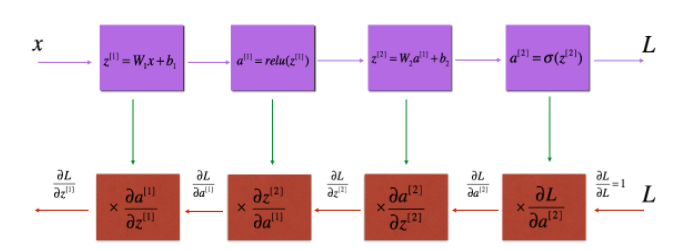
\includegraphics[scale=.6]{deep_back_prop} \vspace*{1mm} \\
	Just like with forward propagation, you will implement helper functions for \textbf{back propagation}. Remember that back propagation is used to calculate the gradient of the loss function with respect to the parameters. We are going to build the backward propagation in three steps: \\
	\hspace*{3mm} 1) LINEAR backward \\
	\hspace*{3mm} 2) LINEAR $\rightarrow$ ACTIVATION backward where ACTIVATION computes the derivative of either the \\ \hspace*{7.5mm} ReLU or sigmoid activation\\
	\hspace*{3mm} 3) [LINEAR $\rightarrow$ RELU] $\times$ (L-1) $\rightarrow$ LINEAR $\rightarrow$ SIGMOID backward (whole model). \\~\\
	Lets begin with step 1. For layer \textit{l}, the linear part is $Z^{[l]}$ followed by an activation. Suppose you have already calculated the derivative $dZ^{[l]} = \frac{\partial \mathcal{L} }{\partial Z^{[l]}}$. You want to get $(dW^{[l]}, db^{[l]}, dA^{[l-1]})$. The process and formulas for this step are: \vspace*{1mm} \\
	\begin{minipage}[c]{9cm}
	$$ dW^{[l]} = \frac{\partial \mathcal{J} }{\partial W^{[l]}} = \frac{1}{m} dZ^{[l]} A^{[l-1] T}$$
	$$ db^{[l]} = \frac{\partial \mathcal{J} }{\partial b^{[l]}} = \frac{1}{m} \sum_{i = 1}^{m} dZ^{[l](i)}$$
	$$ dA^{[l-1]} = \frac{\partial \mathcal{L} }{\partial A^{[l-1]}} = W^{[l] T} dZ^{[l]}$$
	\end{minipage}
	\begin{minipage}[c]{8cm}
	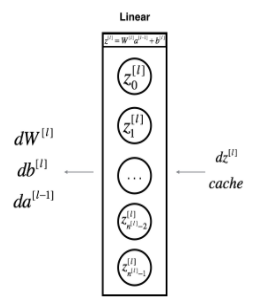
\includegraphics[scale=.9]{linear_back}
	\end{minipage} \newpage
%%%% PAGE 24 %%%%

	\begin{lstlisting}
	def linear_backward(dZ, cache):
		"""
		Implement the linear portion of backward propagation for a single layer (layer l)
		
		Arguments:
		dZ -- Gradient of the cost with respect to the linear output (of current layer l)
		cache -- (A_prev, W, b) coming from the forward propagation in the current layer
		
		Returns:
		dA_prev -- Gradient of the cost with respect to the activation (of the previous 
		           layer l-1), same shape as A_prev
		dW -- Gradient of the cost with respect to W (current layer l), same shape as W
		db -- Gradient of the cost with respect to b (current layer l), same shape as b
		"""
		A_prev, W, b = cache
		m = A_prev.shape[1]
		
		dW = (1/m) * np.dot(dZ, A_prev.T)
		db = (1/m) * np.sum(dZ, axis=1, keepdims=True)
		dA_prev = np.dot(W.T, dZ)

		return dA_prev, dW, db \end{lstlisting} \vspace*{1mm}
	For step 2, we want to write a function that uses linear\_backward and also computes the backward step for the activation function. The sigmoid\_backward and relu\_backward are both pre-built functions (\href{https://www.kaggle.com/kolisnehar/dnn-utils-v2}{click here for details}). If \textit{g} is the activation function, the two pre-built functions compute: $$dZ^{[l]} = dA^{[l]} * g'(Z^{[l]}) $$
	\begin{lstlisting}
	def linear_activation_backward(dA, cache, activation):
		"""
		Implement the backward propagation for the LINEAR->ACTIVATION layer.
		
		Arguments:
		dA -- post-activation gradient for current layer l 
		cache -- (linear_cache, activation_cache) we store for computing backward 
		         propagation efficiently
		activation -- stored as a text string: "sigmoid" or "relu"
		
		Returns:
		dA_prev -- Gradient of the cost with respect to the activation of the previous 
		           layer
		dW -- Gradient of the cost with respect to W (current layer l), same shape as W
		db -- Gradient of the cost with respect to b (current layer l), same shape as b
		"""
		linear_cache, activation_cache = cache
		
		if activation == "relu":
			dZ = relu_backward(dA, activation_cache)
			dA_prev, dW, db = linear_backward(dZ, linear_cache) 
		
		elif activation == "sigmoid":
			dZ = sigmoid_backward(dA, activation_cache)
			dA_prev, dW, db = linear_backward(dZ, linear_cache)
		
		return dA_prev, dW, db	\end{lstlisting} \newpage
%%%% PAGE 25 %%%%

	\noindent For step 3, we will implement the backward function for the whole network. Recall that when you implemented the `L\_model\_forward' function, at each iteration, you stored a cache which contains (X, W, b, and z). In the back propagation module, you will use those variables to compute the gradients. Therefore, in the `L\_model\_backward' function, you will iterate through all the hidden layers backward, starting from layer $L$. On each step, you will use the cached values for layer $l$ to back propagate through layer $l$.
	\begin{minipage}[c]{8.3cm}
	To initialize back propagation, we need the derivative of $A^{[L]}$. Through calculus, we find that this value is $-(\frac{Y}{AL} - \frac{1-Y}{1-AL})$. We can then feed this into linear\_activation\_backward using `sigmoid'. After that, we loop through and compute linear\_activation\_backward using `relu' for all other layers.
	\end{minipage}
	\begin{minipage}[c]{9cm}
	\hspace*{6mm} 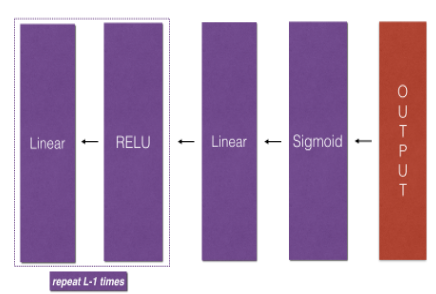
\includegraphics[scale=.7]{l_back_prop}
	\end{minipage} \\
	\begin{lstlisting}
	def L_model_backward(AL, Y, caches):
		"""
		Implement the backward propagation for the [LINEAR->RELU] * (L-1) -> LINEAR -> SIGMOID group
		
		Arguments:
		AL -- probability vector, output of the forward propagation (L_model_forward())
		Y -- true "label" vector (containing 0 if non-cat, 1 if cat)
		caches -- list of caches containing:
		every linear_activation_forward() with "relu" (caches[l] for l in range o to (L-2))
		the cache of linear_activation_forward() with "sigmoid" (it's caches[L-1])
		
		Returns:
		grads -- A dictionary with the gradients
		grads["dA" + str(l)] = ... 
		grads["dW" + str(l)] = ...
		grads["db" + str(l)] = ... 
		"""
		grads = {}
		L = len(caches) # the number of layers
		m = AL.shape[1]
		Y = Y.reshape(AL.shape) # after this line, Y is the same shape as AL
		
		# Initializing the backpropagation
		dAL = - (np.divide(Y, AL) - np.divide(1 - Y, 1 - AL))
		
		# Lth layer (SIGMOID -> LINEAR) gradients.
		current_cache = caches[L-1]
		grads["dA" + str(L-1)], grads["dW" + str(L)], grads["db" + str(L)] = 
		         linear_activation_backward(dAL, current_cache, 'sigmoid')
		
		for l in reversed(range(L-1)): # Loop from l=L-2 to l=0
			# lth layer: (RELU -> LINEAR) gradients.
			current_cache = caches[l]
			dA_prev_temp, dW_temp, db_temp = linear_activation_backward(grads['dA'+str(l+1)], 
			                                                            current_cache,'relu')
			grads["dA" + str(l)] = dA_prev_temp
			grads["dW" + str(l + 1)] = dW_temp
			grads["db" + str(l + 1)] = db_temp
		
		return grads \end{lstlisting} \newpage
%%%% PAGE 25 %%%%

	\noindent The final part of our model is to \textbf{update the parameters} using gradient descent. Recall that: $$ W^{[l]} = W^{[l]} - \alpha \text{ } dW^{[l]}$$ $$ b^{[l]} = b^{[l]} - \alpha \text{ } db^{[l]}$$ where $\alpha$ is the learning rate. After computing the updated parameters, store them in the parameters dictionary. We will use a loop to perform this on every \textit{l} layer.
	\begin{lstlisting}
	def update_parameters(parameters, grads, learning_rate):
		"""
		Update parameters using gradient descent
		
		Arguments:
		parameters -- python dictionary containing your parameters 
		grads -- python dictionary containing your gradients, output of L_model_backward
		
		Returns:
		parameters -- python dictionary containing your updated parameters 
		parameters["W" + str(l)] = ... 
		parameters["b" + str(l)] = ...
		"""
		L = len(parameters) // 2 # number of layers in the neural network
		
		# Update rule for each parameter.
		for l in range(L):
			parameters["W" + str(l+1)] = parameters["W" + str(l+1)] - learning_rate * 
			                             grads["dW" + str(l+1)]
			parameters["b" + str(l+1)] = parameters["b" + str(l+1)] - learning_rate * 
			                             grads["db" + str(l+1)]
		return parameters \end{lstlisting} \vspace*{8mm}
	
	\subsubsection{Programming Assignment 2 (Classifier)}
	You will use the functions you'd implemented in the previous assignment to build a deep network, and apply it to cat vs non-cat classification. Lets start by importing all the packages we will need to use. 
	\begin{lstlisting}
	import time
	import numpy as np
	import h5py
	import matplotlib.pyplot as plt
	import scipy
	from PIL import Image
	from scipy import ndimage
	from dnn_app_utils_v3 import *
	
	%matplotlib inline
	plt.rcParams['figure.figsize'] = (5.0, 4.0) # set default size of plots
	plt.rcParams['image.interpolation'] = 'nearest'
	plt.rcParams['image.cmap'] = 'gray'
	
	%load_ext autoreload
	%autoreload 2
	
	np.random.seed(1) \end{lstlisting} \newpage
%%%% PAGE 27 %%%%

	\noindent \textbf{Problem Statement}: You are given a dataset (``data.h5") containing: \\
	\hspace*{3mm} - a training set of m\_train images labeled as cat (1) or non-cat (0) \\
	\hspace*{3mm} - a test set of m\_test images labeled as cat and non-cat \\
	\hspace*{3mm} - each image is of shape (num\_px, num\_px, 3) where 3 is for the 3 channels (RGB). \vspace*{2mm} \\
	\hspace*{50mm} 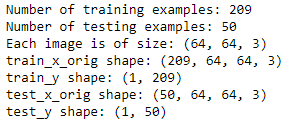
\includegraphics[scale=.8]{cat_shape}
	\begin{lstlisting}
	train_x_orig, train_y, test_x_orig, test_y, classes = load_data()
	
	m_train = train_x_orig.shape[0] # 209
	num_px = train_x_orig.shape[1] # 64, image size = (64, 64, 3)
	m_test = test_x_orig.shape[0] # 50 \end{lstlisting} \vspace*{1mm} 
	\hspace*{35mm} 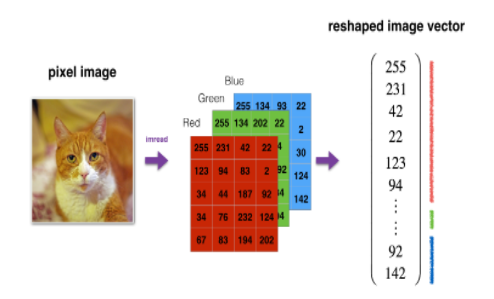
\includegraphics[scale=.7]{cat_stand} \\
	As usual, you \textbf{reshape} and \textbf{standardize} the images before feeding them to the network. For the .reshape() method, the ``-1" makes reshape flatten the remaining dimensions. For the shape, 12288 = 64 x 64 x 3, which is the size of one reshaped image vector.
	\begin{lstlisting}
	# Reshape the training and test examples 
	train_x_flatten = train_x_orig.reshape(train_x_orig.shape[0], -1).T
	test_x_flatten = test_x_orig.reshape(test_x_orig.shape[0], -1).T
	
	# Standardize data to have feature values between 0 and 1.
	train_x = train_x_flatten/255. # shape = (12288, 209)
	test_x = test_x_flatten/255. # shape = (12288, 50)	\end{lstlisting} \vspace*{1mm} 
	We will start with the \textbf{2-Layer Neural Network}. We can see the architecture below: \\	
	\hspace*{30mm} 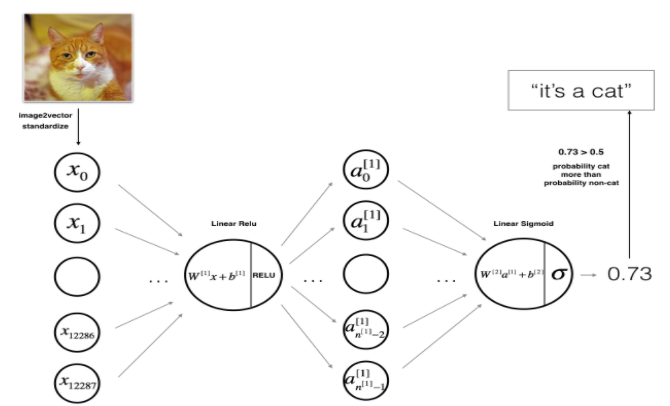
\includegraphics[scale=.6]{two_layer_cat} \newpage
%%%% PAGE 28 %%%%

	\noindent Detailed architecture of above Two-Layer NN figure: \\
	\hspace*{3mm} - The input is a (64,64,3) image which is flattened to a vector of size $(12288,1)$.  \\
	\hspace*{3mm} - The corresponding vector: $[x_0,x_1,...,x_{12287}]^T$ is then multiplied by $W^{[1]}$ of size $(n^{[1]}, 12288)$. \\
	\hspace*{3mm} - You then add a bias term and take its relu to get the following vector: $[a_0^{[1]}, a_1^{[1]},..., a_{n^{[1]}-1}^{[1]}]^T$. \\
	\hspace*{3mm} - You then repeat the same process. \\
	\hspace*{3mm} - You multiply the resulting vector by $W^{[2]}$ and add your intercept (bias).  \\
	\hspace*{3mm} - Finally, you take the sigmoid of the result. If it is greater than 0.5, you classify it to be a cat. \\~\\
	We will follow the general \textbf{methodology} to build the model: \\
	\hspace*{3mm} 1. Initialize parameters / define hyperparameters \\
	\hspace*{3mm} 2. Loop for num\_iterations: \\
	\hspace*{7mm} a. Forward propagation \\
	\hspace*{7mm} b. Compute cost function \\
	\hspace*{7mm} c. Backward propagation \\
	\hspace*{7mm} d. Update parameters (using parameters, and grads from backprop)  \\
	\hspace*{3mm} 3. Use trained parameters to predict labels
	\begin{lstlisting}
	### CONSTANTS DEFINING THE MODEL ####
	n_x = 12288 # num_px * num_px * 3
	n_h = 7
	n_y = 1
	layers_dims = (n_x, n_h, n_y) # (12288, 7, 1)
	
	def two_layer_model(X, Y, layers_dims, learning_rate = 0.0075, num_iterations = 3000, 
	                    print_cost=False):
		"""
		Implements a two-layer neural network: LINEAR->RELU->LINEAR->SIGMOID.
		
		Arguments:
		X -- input data, of shape (n_x, number of examples)
		Y -- true "label" vector (containing 1 if cat, 0 if non-cat), of shape (1, m)
		layers_dims -- dimensions of the layers (n_x, n_h, n_y)
		num_iterations -- number of iterations of the optimization loop
		learning_rate -- learning rate of the gradient descent update rule
		print_cost -- If set to True, this will print the cost every 100 iterations 
		
		Returns:
		parameters -- a dictionary containing W1, W2, b1, and b2
		"""
		np.random.seed(1)
		grads = {}
		costs = [] # to keep track of the cost
		m = X.shape[1] # number of examples
		(n_x, n_h, n_y) = layers_dims
		
		parameters = initialize_parameters(n_x, n_h, n_y) # Initialize parameters dict
		
		# Get W1, b1, W2 and b2 from the dictionary parameters.
		W1 = parameters["W1"]
		b1 = parameters["b1"]
		W2 = parameters["W2"]
		b2 = parameters["b2"]
		
		# Loop (gradient descent)
		for i in range(0, num_iterations):
			# Forward propagation: LINEAR -> RELU -> LINEAR -> SIGMOID
			A1, cache1 = linear_activation_forward(X, W1, b1, 'relu')
			A2, cache2 = linear_activation_forward(A1, W2, b2, 'sigmoid') \end{lstlisting} \newpage
%%%% PAGE 29 %%%%
			
	\begin{lstlisting}
			# Compute cost
			cost = compute_cost(A2, Y)
			
			# Initializing backward propagation
			dA2 = - (np.divide(Y, A2) - np.divide(1 - Y, 1 - A2))
			
			# Backward propagation
			dA1, dW2, db2 = linear_activation_backward(dA2, cache2, 'sigmoid')
			dA0, dW1, db1 = linear_activation_backward(dA1, cache1, 'relu')
			
			# Set grads to corresponding values
			grads['dW1'] = dW1
			grads['db1'] = db1
			grads['dW2'] = dW2
			grads['db2'] = db2
			
			# Update parameters.
			parameters = update_parameters(parameters, grads, learning_rate)
			
			# Retrieve W1, b1, W2, b2 from parameters
			W1 = parameters["W1"]
			b1 = parameters["b1"]
			W2 = parameters["W2"]
			b2 = parameters["b2"]
			
			# Print the cost every 100 training example
			if print_cost and i % 100 == 0:
				print("Cost after iteration {}: {}".format(i, np.squeeze(cost)))
			if print_cost and i % 100 == 0:
				costs.append(cost)
		
		# plot the cost
		plt.plot(np.squeeze(costs))
		plt.ylabel('cost')
		plt.xlabel('iterations (per hundreds)')
		plt.title("Learning rate =" + str(learning_rate))
		plt.show()
		
		return parameters \end{lstlisting} \vspace*{1mm}
	Now that we have a working model we can train the parameters, use them to classify images, and determine our accuracy. *Note*: You may notice that running the model on fewer iterations (say 1500) gives better accuracy on the test set. This is called \textit{early stopping}and we will talk about it in the next course. Early stopping is a way to prevent overfitting. 
	\begin{lstlisting}
	parameters = two_layer_model(train_x, train_y, layers_dims = (n_x, n_h, n_y), 
	                             num_iterations = 2500, print_cost=True)
	
	predictions_train = predict(train_x, train_y, parameters) # Accuracy = 1.0
	predictions_test = predict(test_x, test_y, parameters) # 0.72	\end{lstlisting} \vspace*{1mm}
	\begin{minipage}[c]{8.3cm}
	\hspace*{6mm} 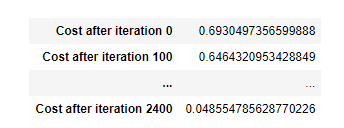
\includegraphics[scale=.9]{cost_cat_2}
	\end{minipage}
	\begin{minipage}[c]{9cm}
	\hspace*{17mm} 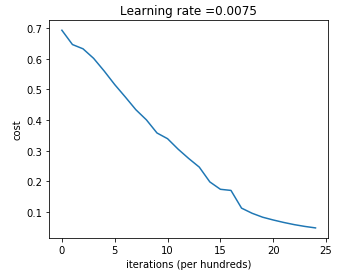
\includegraphics[scale=.6]{lr_graph_2}
	\end{minipage} \newpage
%%%% PAGE 30 %%%%

	\noindent Now that we have created a two-layer Neural Network, lets take a look at how to implement a \textbf{L-Layer Neural Network}. Below is the general architecture we will use: \\
	\hspace*{17mm} 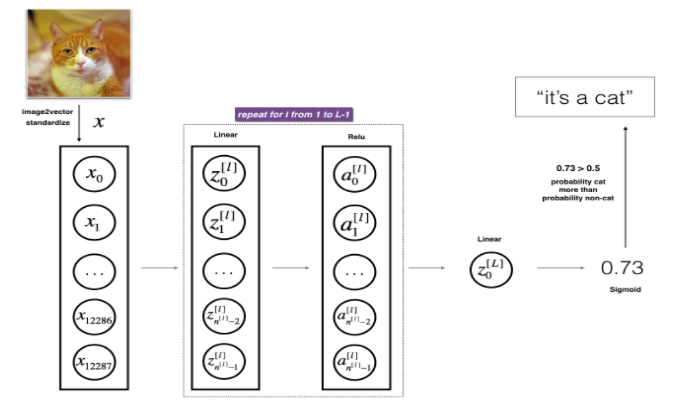
\includegraphics[scale=.7]{l_layer_cat} \\
	Detailed architecture of L-Layer NN: \\
	\hspace*{3mm} - The input is a (64,64,3) image which is flattened to a vector of size (12288,1). \\
	\hspace*{3mm} - The corresponding vector: $[x_0,x_1,...,x_{12287}]^T$ is then multiplied by the weight matrix $W^{[1]}$ and then \hspace*{6mm} you add the intercept $b^{[1]}$. The result is called the linear unit. \\
	\hspace*{3mm} - Next, you take the relu of the linear unit. This process could be repeated several times for each \\ \hspace*{6mm} $(W^{[l]}, b^{[l]})$ depending on the model architecture. \\
	\hspace*{3mm} - Finally, you take the sigmoid of the final linear unit. If it is greater than 0.5, you classify it as a cat.
	\begin{lstlisting}
	### CONSTANTS ###
	layers_dims = [12288, 20, 7, 5, 1] #  4-layer model
	
	def L_layer_model(X, Y, layers_dims, learning_rate = 0.0075, num_iterations = 3000, print_cost=False):#lr was 0.009
		"""
		Implements a L-layer neural network: [LINEAR->RELU]*(L-1)->LINEAR->SIGMOID.
		
		Arguments:
		X -- data, numpy array of shape (num_px * num_px * 3, number of examples)
		Y -- true "label" vector (containing 0 if cat, 1 if non-cat), of shape (1, m)
		layers_dims -- list containing the input size and each layer size, of length (L+1).
		learning_rate -- learning rate of the gradient descent update rule
		num_iterations -- number of iterations of the optimization loop
		print_cost -- if True, it prints the cost every 100 steps
		
		Returns:
		parameters -- parameters learnt by the model. They can then be used to predict.
		"""
		np.random.seed(1)
		costs = [] # keep track of cost
		
		parameters = initialize_parameters_deep(layers_dims) # Parameters initialization
		
		for i in range(0, num_iterations): # Loop (gradient descent)
			AL, caches = L_model_forward(X, parameters) # Forward propagation

			cost = compute_cost(AL, Y) # Compute cost
			
			grads = L_model_backward(AL, Y, caches) # Backward propagation.
			
			parameters = update_parameters(parameters, grads, learning_rate) # Update params.\end{lstlisting} \newpage
%%%% PAGE 31 %%%%
			
	\begin{lstlisting}			
			# Print the cost every 100 training example
			if print_cost and i % 100 == 0:
				print ("Cost after iteration %i: %f" %(i, cost))
			if print_cost and i % 100 == 0:
				costs.append(cost)
		
		# plot the cost
		plt.plot(np.squeeze(costs))
		plt.ylabel('cost')
		plt.xlabel('iterations (per hundreds)')
		plt.title("Learning rate =" + str(learning_rate))
		plt.show()
		
		return parameters \end{lstlisting} \vspace*{1mm}
	With our working model we can now \textbf{train} the parameters and make \textbf{predictions} to determine our accuracy.
	\begin{lstlisting}
	parameters = L_layer_model(train_x, train_y, layers_dims, num_iterations = 2500, 
	                           print_cost = True)
				
	pred_train = predict(train_x, train_y, parameters) # Accuracy: 0.985645933014
	pred_test = predict(test_x, test_y, parameters) # Accuracy: 0.8	\end{lstlisting} \vspace*{1mm}
	It seems that your 4-layer neural network has better performance (80\%) than your 2-layer neural network (72\%) on the same test set. This is good performance for this task. Though in the next course on ``Improving deep neural networks" you will learn how to obtain even higher accuracy by systematically searching for better hyperparameters (learning\_rate, layers\_dims, num\_iterations, and others you'll also learn in the next course). \newpage
%%%% PAGE 32 %%%%

	\section{Improving Deep Neural Networks}
	\subsection{Regularizing \& Optimizing Your Neural Network}
	\subsubsection{Bias/Variance}
	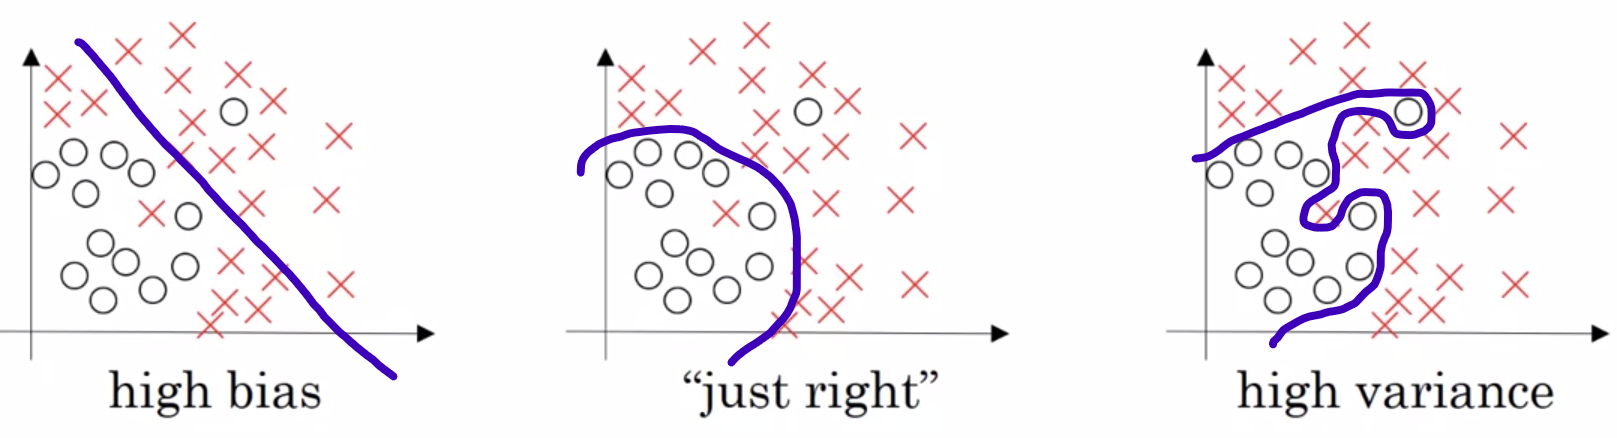
\includegraphics[scale=.4]{bias_var} \\
	\hspace*{3mm} - \textit{High Bias} leads to \textbf{underfitting}, where it cannot find distinct trends in the data. \\
	\hspace*{3mm} - ``\textit{Just right}" is where we aim to be, where our model is fitted but not too close. \\
	\hspace*{3mm} - \textit{High Variance} leads to \textbf{overfitting}, where it is fit too close to the data. \vspace*{1mm} \\
	Lets take a look at an example for a cat classification model. We know that humans will have approximately 0\% error, so we say that the \textbf{Optimal (Bayes) error} is approximately 0\% as well. For the following errors, we say:
	\begin{center}
	\begin{tabular}{ |c|c|c|c|c| } 
	\hline
	Train Set Error & 1\% & 15\% & 15\% & 0.5\% \\  \hline
	Dev Set Error & 11\% & 16\% & 30\% & 1\% \\  \hline
	 & High Var & High Bias & High Var \& Bias & Low Var \& Bias \\ \hline
	\end{tabular}
	\end{center}
	A general rule is that you look at the \textit{training set error} to get an understanding of how bad your \textbf{bias} is. Then, looking at how much higher your \textit{dev set error} will give you an idea of how high your \textbf{variance} is. All of this is made under the assumption that your Bayes error is quite small and your training/dev sets are drawn from the same distribution. \\~\\
	When training a Neural Network, we want to following these \textbf{general guidelines}: \vspace*{.5mm} \\
	\hspace*{3mm} 1) Does the algorithm have high bias? (look at training data performance). \\
	\hspace*{7mm} - Possible Solutions: Bigger network (more $n_h$), train longer, different NN architecture. \\
	\hspace*{3mm} 2) Once bias is reduce, check for a variance problem. (look at dev set data performance). \\
	\hspace*{7mm} - Possible Solutions: More data, Regularization, different NN architecture. \vspace*{1.5mm} \\
	There used to be a ``\textit{bias variance trade-off}", where an increase/decrease in one aspect would result in the opposite effect for the other aspect. However, nowadays this is no longer the case. As long as we can get more data to \textit{decrease} our variance, as well as train a bigger network to \textit{decrease} bias, both aspects will decrease instead of having a trade-off. 
	\subsubsection{Regularization}
	If you suspect that your Neural Network is \textit{overfitting} your data, meaning you have a high variance problem, one of the first things you should try is \textbf{Regularization}. \vspace*{1mm} \\ Lets first look at this idea in terms of Logistic Regression. Recall that we want to find the min of \textit{J}(w,b). We  can do this by adding a \textit{regularization parameter} ($\lambda$) multiplied by the \textit{norm} of w squared ($||w||^2$). $$ J(w,b) = \frac{1}{m} \sum_{i=1}^{m} L(\hat{y}^{(i)}, y^{(i)}) + \frac{\lambda}{2m} ||w||^2_2$$ \newpage
%%%% PAGE 33 %%%%

	\noindent Above, the norm of w squared is called $L_2$ \textit{regularization}: $||w||^2_2 = \sum_{j=1}^{n_x} w^2_j = w^Tw$ \vspace*{1.5mm} \\
	The \textbf{regularization parameter ($\lambda$)} is usually set with the dev set by using \textit{cross-validation}, where you try a variety of values and see which performs the best. \\~\\
	To regularize over a Neural Network, we use the \textbf{Forbenius norm} (weight decay) of a matrix:
	$$ J(w^{[1]}, b^{[1]}, ..., w^{[L]}, b^{[L]}) = \frac{1}{m} \sum_{i=1}^{m} L(\hat{y}^{(i)}, y^{(i)}) + \frac{\lambda}{2m} \sum_{l=1}^{L} ||W^{[l]}||^2_F$$ $$ ||W^{[l]}||^2_F = \sum_{i=1}^{n^l}\sum_{j=1}^{n^{[l-1]}} (W^{[l]}_{i,j})^2$$ 
	The rows ``i" of the matrix should be the number of neurons in the current layer $n^{[l]}$, whereas the columns ''j" of the weight matrix should equal the number of neurons in the previous layer $n^{[l-1]}$. \vspace*{1mm} \\
	To implement \textbf{gradient descent}, we know use these updated formulas: 
	$$ dW^{[l]} = (backprop) + \frac{\lambda}{m}W^{[l]} $$
	$$ W^{[l]} = W^{[l]} - \alpha\, dW^{[l]} $$
	The way the regularization prevents overfitting is that the larger the $\lambda$ value is, the closer the weight matrix will be to 0. Doing this will move you from high variance (right picture in above diagram) to high bias (left picture above). The concept is that the $\lambda$ value will result to the ``just right'' case (middle picture). The $\lambda$ value causes hidden units to have a much smaller impact, so it leads to a simpler/smaller network that is less prone to overfitting. \vspace*{1mm} \\
	One example is by using tanh as our activation function, having a large $\lambda$ value will cause $W^{[l]}$ to be smaller, meaning that $z^{[l]}$ will also be smaller (range of values will be reduced and more focused in the middle around 0). This causes every layer to be approximately linear, meaning that it will cause less overfitting by preventing complex decision boundaries and using a straighter line for the boundary. 
	\subsubsection{Dropout Regularization}
	\begin{center} 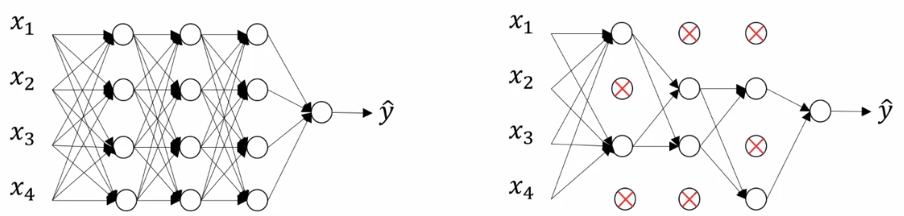
\includegraphics[scale=.6]{dropout_reg}	\end{center}
	\textbf{Dropout regularization} is used to reduce Neural Networks by randomly choosing hidden units to remove from a Network, along with removing all inputs/outputs coming from the removed nodes. You do this for each training example, so each example \textit{i} is trained on a different reduced Neural Network. \vspace*{1.5mm} \\
	One way to implement dropout regularization is called \textbf{inverted dropout}. Lets use \textit{l} = 3.
	\begin{lstlisting}
	keep_prob = 0.8 # can be any value in range (0,1)
	d3 = np/random.rand(a3.shape[0], a3.shape[1]) < keep_prob # boolean array
	a3 = np.multiply(a3, d3) # reduce activation for 0 valued d3 nodes (20% reduced)
	a3 /= keep_prob # bumps values up by 20% so we dont change expected value for z4 \end{lstlisting} \vspace*{1mm}
	Note that when make predictions on the test data, we use the dropout activation matrices. We do not want to calculate these values at test time because it will add noise to our predictions. \newpage
%%%% PAGE 34 %%%%

	\noindent A few other forms of regularization that we can use are: \vspace*{.5mm} \\
	\hspace*{3mm} - Data Augmentation : manipulating the data (ex: flipping/cropping an image) to create more data. \\
	\hspace*{3mm} - Early stopping : during gradient descent, we stop training when we hit a certain value. \vspace*{1mm} \\
	\textbf{Orthogonalization} tells us that we only want to focus on one task at a time. The first and most important is optimizing the cost function \textit{J} so that we minimize \textit{J}(w,b). The second is then to not overfit our data, i.e. using regularization techniques in order to do this. $L_2$ regularization, even though you have to try a lot of values for $\lambda$ and can be more expensive with larger models, is still better than early stopping. 
	\subsubsection{Normalizing Inputs}
	One technique used to speed up our training is if we \textbf{normalize} our inputs. We can do this in two steps:\vspace*{.5mm} \\
	\hspace*{3mm} 1) Subtract the mean, $\mu = \sum_{i=1}^{m} x^{(i)}$, from each training example so that x = x - $\mu$ \\
	\hspace*{3mm} 2) Normalize the variance, $\sigma = \frac{1}{m} \sum_{i=1}^{m} x^{(i)} ** 2 $, element-wise squared, so that x /= $\sigma$ \\ $$ \frac{x- \mu}{\sigma} $$
	\begin{center} 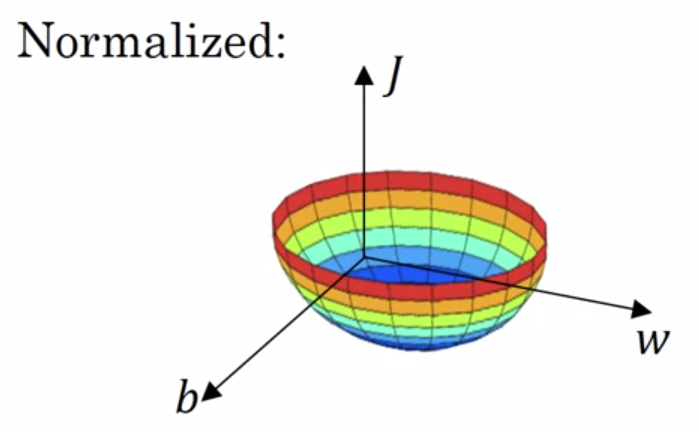
\includegraphics[scale=.35]{normalized_in} \hspace*{10mm} 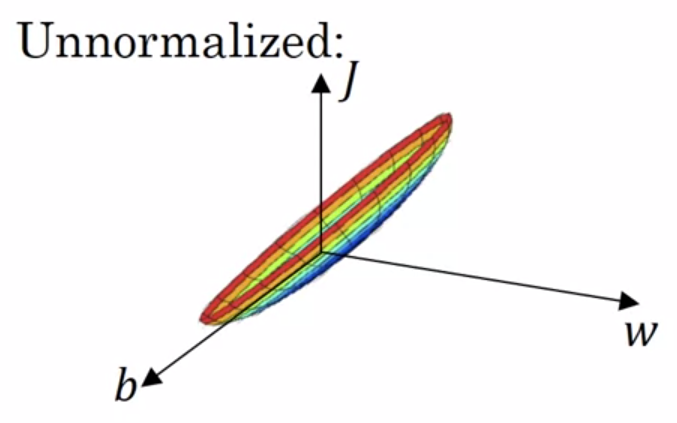
\includegraphics[scale=.35]{unnormalized_in} \end{center}
	We want to normalize our data because if we don't, then the cost function can be a very elongated. But if we normalize, then our cost function will be more symmetrical and need less steps for gradient descent (it can go straight to a minimum rather than oscillating). 
	\subsubsection{Weight Initialization}
	When you begin to use much deeper Neural Networks with many hidden layers, you want to be careful in you choice of random initialization for the weights matrix. Lets first take a look at an example for a single neuron:
	\begin{center} 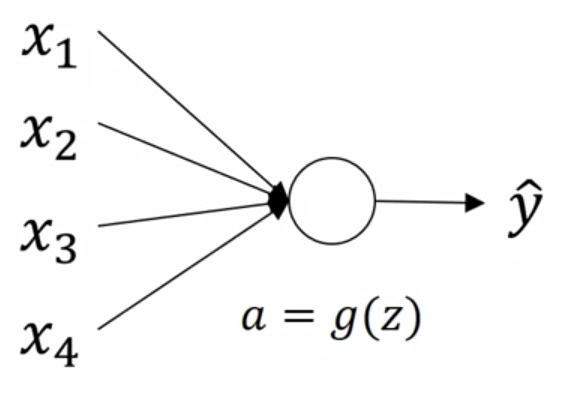
\includegraphics[scale=.4]{single_neuron} \\ \end{center} 
	We know that $z = w_1x_1 + w_2x_2 + ... + w_nx_n$ and we will set b=0. In order to make z not explode/shrink, we want will conclude that the larger \textit{n} is, the smaller we want $w_i$ to be. We can do this by setting the $Var(w_i) = \frac{1}{n}$. Note that if your are using a ReLU function, then we want $Var(w_i) = \frac{2}{n}$. In Python, the general formula for ReLU we use would be: $$ W^{[l]} = np.random.randn(shape) * np.sqrt(\frac{2}{n^{[l-1]}})$$ \newpage
%%%% PAGE 35 %%%%

	\subsubsection{Gradient Checking}
	When you implement back propagation you'll find that there's a test called \textbf{gradient checking} that can help you make sure that your implementation of back prop is correct. In order to build up to this, lets first talk about how to \textit{numerically approximate computations of gradients}. \vspace*{1mm} \\
	\begin{minipage}[c]{7cm}
	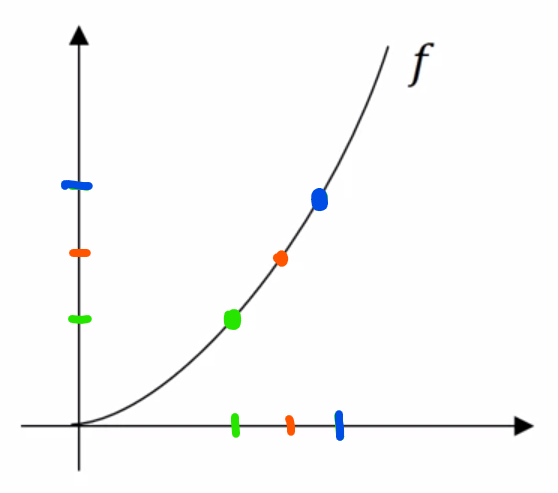
\includegraphics[scale=.4]{num_grad_check}
	\end{minipage}
	\begin{minipage}[c]{9cm}
	We know that: \\
	$f(\theta) = \theta^3$ \\ $\epsilon$ = 0.01 \\ Green x-axis = $\theta - \epsilon$ = 0.99 \\ Blue x-axis = $\theta + \epsilon$ = 1.01 \\ Red x-axis = $\theta$ = 1 \\ Green y-axis = $f(\theta-\epsilon)$ \\ Blue y-axis = $f(\theta+\epsilon)$ \\ Red y-axis = $f(\theta)$
	\end{minipage} \\
	We want to find the gradient for the triangle created by the green and blue dot. This means that the \textit{height} = $f(\theta+\epsilon) - f(\theta-\epsilon)$, and the \textit{width} = $2\epsilon$. This means that: $$ g(\theta) = \frac{f(\theta+\epsilon) - f(\theta-\epsilon)}{2\epsilon} $$ 
	If we plug in our values from above, we would see our \textbf{two-sided} gradient = 3.0001 (error = 0.0001). If we had done it how we had previously using a \textbf{one-sided} approach (only using $\theta$ and $\theta+\epsilon$ for our triangle), our gradient = 3.0301 (error = 0.0301). Note that in code, the two sided approach is twice as slow, but works much better since it is more accurate. Our big-O notation for error is: O($\epsilon^2$). \\~\\
	Now that we've seen that, lest take a look at how to implement \textbf{gradient checking}. We first must:  \\
	\hspace*{3mm} 1) Take $W^{[1]}, b^{[1]},..., W^{[L]}, b^{[L]}$ and reshape (concatenate) into a big vector $\theta$. \\
	\hspace*{7mm} - Note that now, $J(W^{[1]}, b^{[1]},..., W^{[L]}, b^{[L]}) = J(\theta)$. \\
	\hspace*{3mm} 2) Take $dW^{[1]}, db^{[1]},..., dW^{[L]}, db^{[L]}$ and reshape (concatenate) into a big vector $d\theta$. \vspace*{1mm}\\
	Now that we have $d\theta$, we want to see if it is the gradient of $J(\theta)$. In order to find this our, we use the following formula for every \textit{i} (component of $\theta$): $$ d\theta_{approx} = \frac{J(\theta_1, \theta_2,...,\theta_{i+\epsilon},...) - J(\theta_1, \theta_2,...,\theta_{i-\epsilon},...)}{2\epsilon} $$ $$ \approx d\theta[i] = \frac{\partial J}{\partial d\theta_i}$$ 
	The final step is to see if our $d\theta_{approx} \approx d\theta$. We can do this by checking the difference between the two vectors by computing the Euclidean distance and normalizing it: $$ \frac{||d\theta_{approx} - d\theta||_2}{||d\theta_{approx}||_2 - ||d\theta||_2}$$
	If the value outputted by the formula above is similar to the value of $\epsilon$, then we know our back propagation is working. However, the farther away we get from the value, the more we need to go back and check that our implementation is correct. \vspace*{1mm} \\
	Notes on implementation of Gradient checking: \\
	\hspace*{3mm} - Don't use in training, only to debug. \\
	\hspace*{3mm} - If algorithm fails grad check, look at components to try to identify bugs. \\
	\hspace*{3mm} - Remeber regularization (add on regularization term to J($\theta$) in grad check). \\
	\hspace*{3mm} - This does not work with dropout regularization. \newpage
%%%% PAGE 36 %%%%

	\subsubsection{Programming Assignment (Initialization)}
	In this assignment we will see how different initializations lead to different results. You will use a 3-layer neural network (already implemented for you). The initialization methods you will experiment with are: \\
	\hspace*{3mm} - \textit{Zeros initialization} - setting initialization = ``zeros" in the input argument. \\
	\hspace*{3mm} - \textit{Random initialization} - setting initialization = ``random" in the input argument. This initializes the \hspace*{6.5mm} weights to large random values.  \\
	\hspace*{3mm} - \textit{He initialization} - setting initialization = ``he" in the input argument. This initializes the weights \hspace*{6.5mm} to random values scaled according to a paper by He et al., 2015.
	\begin{lstlisting}
	def model(X, Y, learning_rate = 0.01, num_iterations = 15000, print_cost = True, 
	          initialization = "he"):
		"""
		Implements a 3-layer neural network: LINEAR->RELU->LINEAR->RELU->LINEAR->SIGMOID.
		
		Arguments:
		X - input data, of shape (2, number of examples)
		Y - true "label" vector (0 for red dots; 1 for blue dots), of shape (1, m)
		print_cost - if True, print the cost every 1000 iterations
		initialization - flag to choose initialization to use ("zeros","random" or "he")
		"""
		grads = {}
		costs = [] # to keep track of the loss
		m = X.shape[1] # number of examples
		layers_dims = [X.shape[0], 10, 5, 1]
		
		# Initialize parameters dictionary.
		if initialization == "zeros":
			parameters = initialize_parameters_zeros(layers_dims)
		elif initialization == "random":
			parameters = initialize_parameters_random(layers_dims)
		elif initialization == "he":
			parameters = initialize_parameters_he(layers_dims)
		
		# Loop (gradient descent)
		for i in range(0, num_iterations):
			# Forward propagation: LINEAR -> RELU -> LINEAR -> RELU -> LINEAR -> SIGMOID.
			a3, cache = forward_propagation(X, parameters)
			
			cost = compute_loss(a3, Y) # Loss
			
			grads = backward_propagation(X, Y, cache) # Backward propagation.
			
			# Update parameters.
			parameters = update_parameters(parameters, grads, learning_rate)
			
			# Print the loss every 1000 iterations
			if print_cost and i % 1000 == 0:
				print("Cost after iteration {}: {}".format(i, cost))
				costs.append(cost)
		
		# plot the loss
		plt.plot(costs)
		plt.ylabel('cost')
		plt.xlabel('iterations (per hundreds)')
		plt.title("Learning rate =" + str(learning_rate))
		plt.show()
		
		return parameters \end{lstlisting} \newpage
%%%% PAGE 37 %%%%

	\noindent Lets import the packages and planar dataset that we want to classify. \\
	\begin{minipage}[c]{10.5cm}
	\begin{lstlisting}
	import numpy as np
	import matplotlib.pyplot as plt
	import sklearn
	import sklearn.datasets
	
	# load image dataset: blue/red dots in circles
	train_X, train_Y, test_X, test_Y = load_dataset() \end{lstlisting} \vspace*{3mm}
	\end{minipage}
	\begin{minipage}[c]{8cm}
	\hspace*{1mm} 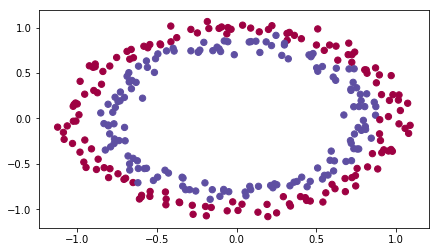
\includegraphics[scale=0.55]{planar_data} \\
	\end{minipage}
	First, lets use \textbf{zero initialization}. There are two types of parameters to initialize in a neural network: \vspace*{1mm}\\
	\hspace*{3mm} - The weight matrices $(W^{[1]}, W^{[2]}, W^{[3]}, ..., W^{[L-1]}, W^{[L]})$ \\
	\hspace*{3mm} - The bias vectors $(b^{[1]}, b^{[2]}, b^{[3]}, ..., b^{[L-1]}, b^{[L]})$ \vspace*{1mm}\\
	You'll see later that this does not work well since it fails to ``break symmetry".
	\begin{lstlisting}
	def initialize_parameters_zeros(layers_dims):
		"""
		layer_dims -- python array (list) containing the size of each layer.
		"""
		parameters = {}
		L = len(layers_dims) # number of layers in the network
		
		for l in range(1, L):
			parameters['W' + str(l)] = np.zeros((layers_dims[l], layers_dims[l-1]))
			parameters['b' + str(l)] = np.zeros((layers_dims[l], 1))
		return parameters  # dict containing: "W1", "b1", ..., "WL", "bL"
	
	parameters = model(train_X, train_Y, initialization = "zeros")
	predictions_train = predict(train_X, train_Y, parameters) # 0.5
	predictions_test = predict(test_X, test_Y, parameters) # 0.5 \end{lstlisting} \vspace*{1mm}
	\begin{minipage}[c]{10.5cm}
	If you were to run the above code, we would see that for each iterations the cost is not changing. The performance is really bad, and if you were to print the predictions for the training/test set, you would see that the algorithm is predicting 0's every time. Initializing the weights to zero fails to break symmetry, and is similar to training on $n^{[l]} = 1$ for every layer. It is only okay to initialize \textit{b} to zeros, but never \textit{W} to zeros.
	\end{minipage}
	\begin{minipage}[c]{8cm}
	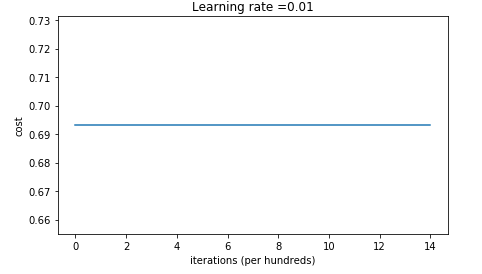
\includegraphics[scale=0.55]{zeros_init} \\
	\end{minipage}
	To break symmetry, lets initialize the weights randomly. Following \textbf{random initialization}, each neuron can then proceed to learn a different function of its inputs. Note that for \textit{W}, we are initializing to large random values scaled by 10.
	\begin{lstlisting}
	def initialize_parameters_random(layers_dims):
		"""
		layer_dims -- python array (list) containing the size of each layer.
		"""
		np.random.seed(3)
		parameters = {}
		L = len(layers_dims) # integer representing the number of layers
		
		for l in range(1, L):
			parameters['W' + str(l)] = np.random.randn(layers_dims[l], layers_dims[l-1]) * 10
			parameters['b' + str(l)] = np.zeros((layers_dims[l], 1))
		
		return parameters \end{lstlisting} \newpage
%%%% PAGE 38 %%%%

	\begin{lstlisting}
	parameters = model(train_X, train_Y, initialization = "random")
	predictions_train = predict(train_X, train_Y, parameters) # 0.83
	predictions_test = predict(test_X, test_Y, parameters) # 0.86
	
	plt.title("Model with large random initialization")
	axes = plt.gca()
	axes.set_xlim([-1.5,1.5])
	axes.set_ylim([-1.5,1.5])
	plot_decision_boundary(lambda x: predict_dec(parameters, x.T), train_X, train_Y)\end{lstlisting} \vspace*{1mm}
	\begin{minipage}[c]{8.5cm}
	\begin{center}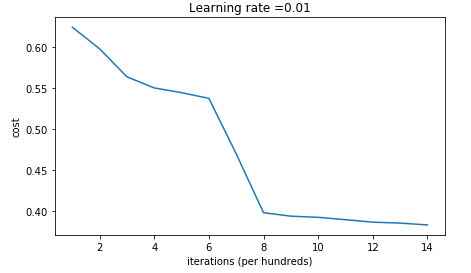
\includegraphics[scale=0.6]{rand_init_large} \end{center}
	\end{minipage}
	\begin{minipage}[c]{8.5cm}
	\begin{center}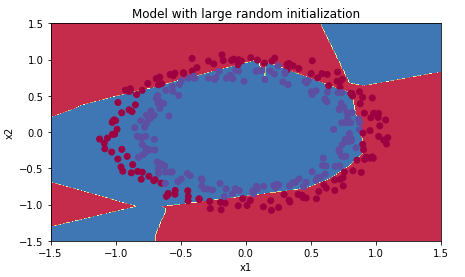
\includegraphics[scale=0.6]{dec_bound_rand} \\ \end{center} 
	\end{minipage} \vspace*{2mm} \newline
	If we were to run the above, although the first iteration (0) is infinity, the cost goes down each 1000 iterations, thus we have broken symmetry. If you train this network longer you will see better results, but initializing with overly large random numbers slows down the optimization. Overall, using very large random value to initialize weights does not work very well. \vspace*{3mm} \\
	Finally, we will try \textbf{He Initialization}. This is very similar to \textit{Xavier Initialization} except instead of using a scaling factor of 1, we use a scaling factor of 2. Note that this is recommended with layers that use a ReLU activation function. We use : $\sqrt{\frac{2}{previous\, layer\, dimensions}}	$
	\begin{lstlisting}
	def initialize_parameters_he(layers_dims):
		# layer_dims -- python array (list) containing the size of each layer.
		np.random.seed(3)
		parameters = {}
		L = len(layers_dims) - 1 # integer representing the number of layers
		
		for l in range(1, L + 1):
			parameters['W' + str(l)] = np.random.randn(layers_dims[l], layers_dims[l-1]) * 
			                           np.sqrt(2/layers_dims[l-1])
			parameters['b' + str(l)] = np.zeros((layers_dims[l], 1))
		
		return parameters
		
	parameters = model(train_X, train_Y, initialization = "he")
	predictions_train = predict(train_X, train_Y, parameters) # 0.993333
	predictions_test = predict(test_X, test_Y, parameters) # 0.96
	
	plt.title("Model with He initialization")
	axes = plt.gca()
	axes.set_xlim([-1.5,1.5])
	axes.set_ylim([-1.5,1.5])
	plot_decision_boundary(lambda x: predict_dec(parameters, x.T), train_X, train_Y) \end{lstlisting}
	\begin{minipage}[c]{8.5cm}
	\begin{center}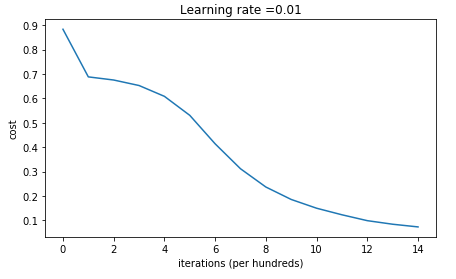
\includegraphics[scale=0.5]{he_init} \end{center}
	\end{minipage}
	\begin{minipage}[c]{8.5cm}
	\begin{center}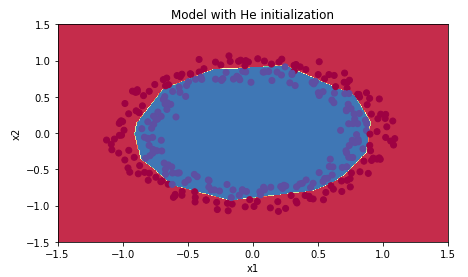
\includegraphics[scale=0.5]{he_init_dec} \end{center} 
	\end{minipage} \newpage
%%%% PAGE 39 %%%%

	\subsubsection{Programming Assignment (Regularization)}
	We will recommend positions where France's goal keeper should kick the ball so that the French team's players can then hit it with their head. We have data from the past 10 games played by the French team. Each dot corresponds to a position on the football field where a football player has hit the ball with his/her head after the French goal keeper has shot the ball from the left side of the football field: \vspace*{1mm} \\
	\hspace*{3mm} - If the dot is blue, it means the French player managed to hit the ball with his/her head. \\
	\hspace*{3mm} - If the dot is red, it means the other team's player hit the ball with their head. \\
	Our goal is to create a deep learning model to find the positions on the field where the goalkeeper should kick the ball. \vspace*{1mm} \\
	\begin{minipage}[c]{8.5cm}
	\begin{center}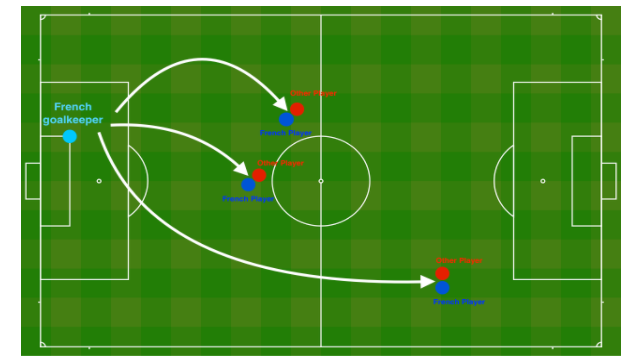
\includegraphics[scale=0.4]{field} \end{center}
	\end{minipage}
	\begin{minipage}[c]{8.5cm}
	\begin{center}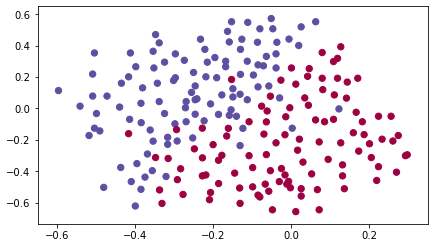
\includegraphics[scale=0.68]{field_graph} \end{center} 
	\end{minipage} \vspace*{1.5mm} \newline
	The dataset is a little noisy, but from a quick glance we can see the a diagonal line would work decent in separating the two data points. \vspace*{1mm} \\
	We will load in the packages that we will need for the project, along with a Neural Network that has already been implemented for us. Note that to use the model in \textit{regularization} mode, we just change the $\lambda$ value to something besides 0. And to use the model in \textit{dropout} mode, we change the keep\_prob to a value below 1. 
	\begin{lstlisting}
	import numpy as np
	import matplotlib.pyplot as plt
	from reg_utils import sigmoid, relu, plot_decision_boundary, initialize_parameters, 
	                      load_2D_dataset, predict_dec
	from reg_utils import compute_cost, predict, forward_propagation, 
	                      backward_propagation, update_parameters
	import sklearn
	import sklearn.datasets
	import scipy.io
	from testCases import *
	
	train_X, train_Y, test_X, test_Y = load_2D_dataset()
	
	
	def model(X, Y, learning_rate = 0.3, num_iterations = 30000, print_cost = True, 
	          lambd = 0, keep_prob = 1):
		"""
		Implements a 3-layer neural network: LINEAR->RELU->LINEAR->RELU->LINEAR->SIGMOID.
		
		Arguments:
		X -- input data, of shape (input size, number of examples)
		Y -- true "label" vector (1 for blue dot / 0 for red dot), of shape (output size,m)
		learning_rate -- learning rate of the optimization
		num_iterations -- number of iterations of the optimization loop
		print_cost -- If True, print the cost every 10000 iterations
		lambd -- regularization hyperparameter, scalar
		keep_prob - probability of keeping a neuron active during drop-out, scalar.
		
		Returns:
		parameters -- parameters learned by the model. They can then be used to predict.
		""" \end{lstlisting} \newpage
%%%% PAGE 40 %%%%

	\begin{lstlisting}
		grads = {}
		costs = [] # to keep track of the cost
		m = X.shape[1] # number of examples
		layers_dims = [X.shape[0], 20, 3, 1]
		
		parameters = initialize_parameters(layers_dims) # Initialize parameters dictionary.
		
		# Loop (gradient descent)
		for i in range(0, num_iterations):
			# Forward propagation: LINEAR -> RELU -> LINEAR -> RELU -> LINEAR -> SIGMOID.
			if keep_prob == 1:
				a3, cache = forward_propagation(X, parameters)
			elif keep_prob < 1:
				a3, cache = forward_propagation_with_dropout(X, parameters, keep_prob)
			
			# Cost function
			if lambd == 0:
				cost = compute_cost(a3, Y)
			else:
				cost = compute_cost_with_regularization(a3, Y, parameters, lambd)
			
			# Backward propagation.
			assert(lambd==0 or keep_prob==1) # only use one or the other
			if lambd == 0 and keep_prob == 1:
				grads = backward_propagation(X, Y, cache)
			elif lambd != 0:
				grads = backward_propagation_with_regularization(X, Y, cache, lambd)
			elif keep_prob < 1:
				grads = backward_propagation_with_dropout(X, Y, cache, keep_prob)
			
			parameters = update_parameters(parameters, grads, learning_rate) # Update params
		
			if print_cost and i % 10000 == 0: # Print the loss every 10000 iterations
				print("Cost after iteration {}: {}".format(i, cost))
			if print_cost and i % 1000 == 0:
				costs.append(cost)
		
		# plot the cost
		plt.plot(costs)
		plt.ylabel('cost')
		plt.xlabel('iterations (x1,000)')
		plt.title("Learning rate =" + str(learning_rate))
		plt.show()
		
		return parameters \end{lstlisting} \vspace*{1mm}
	We first want to train a model with \textbf{no regularization} (baseline model). If you take a look at the decision boundary, you can see the model is overfitting the training set on the noisy points.
	\begin{lstlisting}
	parameters = model(train_X, train_Y)
	predictions_train = predict(train_X, train_Y, parameters) # 0.94786
	predictions_test = predict(test_X, test_Y, parameters) # 0.915 \end{lstlisting}
	\begin{minipage}[c]{9cm}
	\begin{center} 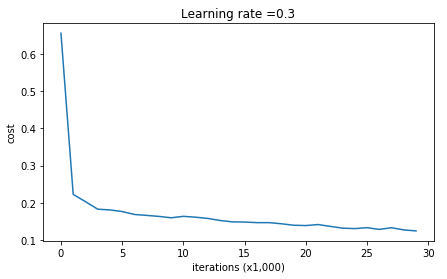
\includegraphics[scale=.51]{no_reg_cost}	\end{center}
	\end{minipage}
	\begin{minipage}[c]{9cm}
	\begin{center} 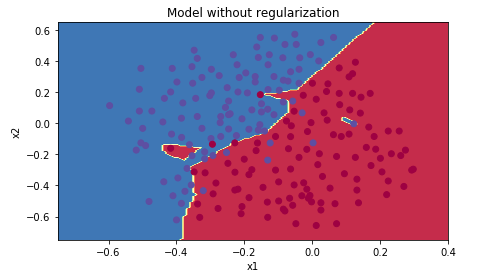
\includegraphics[scale=.51]{no_reg_bound}	\end{center}
	\end{minipage} \newpage
%%%% PAGE 41 %%%%

	\noindent The standard way to avoid overfitting is called \textbf{L2 REGULARIZATION}. It consists of appropriately modifying your cost function, from:	$$J = -\frac{1}{m} \sum\limits_{i = 1}^{m} \large{(}\small  y^{(i)}\log\left(a^{[L](i)}\right) + (1-y^{(i)})\log\left(1- a^{[L](i)}\right) \large{)}$$
	To:
	$$J_{regularized} = \small \underbrace{-\frac{1}{m} \sum\limits_{i = 1}^{m} \large{(}\small y^{(i)}\log\left(a^{[L](i)}\right) + (1-y^{(i)})\log\left(1- a^{[L](i)}\right) \large{)} }_\text{cross-entropy cost} + \underbrace{\frac{1}{m} \frac{\lambda}{2} \sum\limits_l\sum\limits_k\sum\limits_j W_{k,j}^{[l]2} }_\text{L2 regularization cost}$$
	\begin{lstlisting}
	def compute_cost_with_regularization(A3, Y, parameters, lambd):
		"""
		Implement the cost function with L2 regularization. See formula above.
		
		Arguments:
		A3 -- post-activation, output of forward propagation, of shape (output size, m)
		Y -- "true" labels vector, of shape (output size, number of examples)
		parameters -- python dictionary containing parameters of the model
		
		Returns:
		cost - value of the regularized loss function (formula (2))
		"""
		m = Y.shape[1]
		W1 = parameters["W1"]
		W2 = parameters["W2"]
		W3 = parameters["W3"]
		
		cross_entropy_cost = compute_cost(A3, Y) # the cross-entropy part of the cost
		
		L2_regularization_cost = (lambd/(2*m)) * np.sum(np.sum(np.square(W1)) + 
		                         np.sum(np.square(W2)) + np.sum(np.square(W3)))
		
		cost = cross_entropy_cost + L2_regularization_cost
		
		return cost\end{lstlisting} \vspace*{1mm}
	Now, since we have changed the value cost, we must also change backward propagation. All the gradients have to be computed with respect to this new cost. For each, you have to add the regularization term's gradient $$\frac{d}{dW} ( \frac{1}{2}\frac{\lambda}{m}  W^2) = \frac{\lambda}{m} W$$
	\begin{lstlisting}
	def backward_propagation_with_regularization(X, Y, cache, lambd):
		"""
		Implements the backward propagation to which we added an L2 regularization.
		
		Arguments:
		X -- input dataset, of shape (input size, number of examples)
		Y -- "true" labels vector, of shape (output size, number of examples)
		cache -- cache output from forward_propagation()
		lambd -- regularization hyperparameter, scalar
		
		Returns:
		gradients -- Dictionary with gradients and parameters
		"""
		m = X.shape[1]
		(Z1, A1, W1, b1, Z2, A2, W2, b2, Z3, A3, W3, b3) = cache \end{lstlisting} \newpage
%%%% PAGE 42 %%%%
		
	\begin{lstlisting}
		dZ3 = A3 - Y
		dW3 = 1./m * np.dot(dZ3, A2.T) + (lambd/m)*W3
		db3 = 1./m * np.sum(dZ3, axis=1, keepdims = True)
		
		dA2 = np.dot(W3.T, dZ3)
		dZ2 = np.multiply(dA2, np.int64(A2 > 0))
		dW2 = 1./m * np.dot(dZ2, A1.T) + (lambd/m)*W2
		db2 = 1./m * np.sum(dZ2, axis=1, keepdims = True)
		
		dA1 = np.dot(W2.T, dZ2)
		dZ1 = np.multiply(dA1, np.int64(A1 > 0))
		dW1 = 1./m * np.dot(dZ1, X.T) + (lambd/m)*W1
		db1 = 1./m * np.sum(dZ1, axis=1, keepdims = True)
		
		gradients = {"dZ3": dZ3, "dW3": dW3, "db3": db3,"dA2": dA2,
		             "dZ2": dZ2, "dW2": dW2, "db2": db2, "dA1": dA1, 
		             "dZ1": dZ1, "dW1": dW1, "db1": db1}
		
		return gradients \end{lstlisting} \vspace*{1mm}
	Now lets run the model with $\lambda$ = 0.7
	\begin{lstlisting}
	parameters = model(train_X, train_Y, lambd = 0.7)
	predictions_train = predict(train_X, train_Y, parameters) # 0.93838
	predictions_test = predict(test_X, test_Y, parameters) # 0.93 \end{lstlisting} \vspace*{1mm}
	\begin{minipage}[c]{9cm}
	\begin{center} 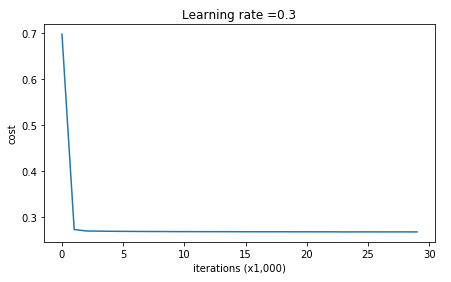
\includegraphics[scale=.51]{l2_reg_cost}	\end{center}
	\end{minipage}
	\begin{minipage}[c]{9cm}
	\begin{center} 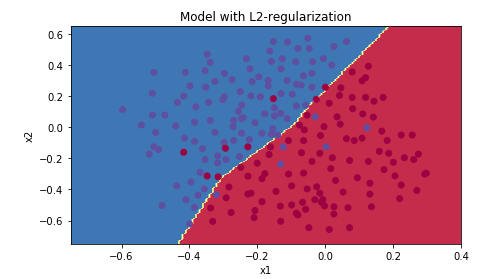
\includegraphics[scale=.51]{l2_reg_bound}	\end{center}
	\end{minipage} \vspace*{1.5mm} \newline
	We have not only increased our accuracy on the test set by 1.5\%, but we are also not longer overfitting the data. Note that L2 regularization makes your decision boundary smoother. If $\lambda$ is too large, it is also possible to ``oversmooth", resulting in a model with high bias. Three key takeaways from this are: \\
	\hspace*{3mm} - The cost computation: A regularization term is added to the cost. \\
	\hspace*{3mm} - The backpropagation function: There are extra terms in the gradients with respect to W. \\
	\hspace*{3mm} - Weights end up smaller ("weight decay") by being pushed to smaller values. \vspace*{2mm} \\~\\
	Finally, \textbf{DROPOUT} is a widely used regularization technique that is specific to deep learning. It randomly shuts down some neurons in each iteration. At each iteration, you shut down (= set to zero) each neuron of a layer with probability $1 - keep\_prob$ or keep it with probability $keep\_prob$. The dropped neurons don't contribute to the training in both the forward and backward propagations of the iteration. \vspace*{1mm} \\
	When you shut some neurons down, you actually modify your model. The idea behind drop-out is that at each iteration, you train a different model that uses only a subset of your neurons. With dropout, your neurons thus become less sensitive to the activation of one other specific neuron, because that other neuron might be shut down at any time.\vspace*{3mm} \\
	The first step is to implement \textit{forward propagation} with dropout. You are using a 3 layer neural network, and will add dropout to the first and second hidden layers. We will not apply dropout to the input layer or output layer. \newpage
%%%% PAGE 43 %%%%

	\begin{lstlisting}
	def forward_propagation_with_dropout(X, parameters, keep_prob = 0.5):
		"""
		Implements the forward propagation: LINEAR -> RELU + DROPOUT -> LINEAR -> 
		                                    RELU + DROPOUT -> LINEAR -> SIGMOID.
		
		Arguments:
		X -- input dataset, of shape (2, number of examples)
		parameters -- python dictionary containing your parameters
		W1 -- weight matrix of shape (20, 2)
		b1 -- bias vector of shape (20, 1)
		W2 -- weight matrix of shape (3, 20)
		b2 -- bias vector of shape (3, 1)
		W3 -- weight matrix of shape (1, 3)
		b3 -- bias vector of shape (1, 1)
		keep_prob - probability of keeping a neuron active during drop-out, scalar
		
		Returns:
		A3 -- last activation value, output of the forward propagation, of shape (1,1)
		cache -- tuple, information stored for computing the backward propagation
		"""
		np.random.seed(1)
		
		# retrieve parameters
		W1 = parameters["W1"]
		b1 = parameters["b1"]
		W2 = parameters["W2"]
		b2 = parameters["b2"]
		W3 = parameters["W3"]
		b3 = parameters["b3"]
		
		# LINEAR -> RELU -> LINEAR -> RELU -> LINEAR -> SIGMOID
		Z1 = np.dot(W1, X) + b1 # linear
		A1 = relu(Z1) # relu
		D1 = np.random.rand(A1.shape[0], A1.shape[1]) # Step 1: initialize matrix D1
		D1 = (D1 < keep_prob).astype(int) # Step 2: convert entries of D1 to 0 or 1
		A1 = A1 * D1 # Step 3: shut down some neurons of A1
		A1 = A1/keep_prob # Step 4: scale the value of neurons that haven't been shut down
		
		Z2 = np.dot(W2, A1) + b2 # linear
		A2 = relu(Z2) # relu
		D2 = np.random.rand(A2.shape[0], A2.shape[1]) # Step 1: initialize matrix D2
		D2 = (D2 < keep_prob).astype(int) # Step 2: convert entries of D2 to 0 or 1
		A2 = A2 * D2  # Step 3: shut down some neurons of A2
		A2 = A2/keep_prob # Step 4: scale the value of neurons that haven't been shut down

		Z3 = np.dot(W3, A2) + b3 # linear
		A3 = sigmoid(Z3) # sigmoid
		
		cache = (Z1, D1, A1, W1, b1, Z2, D2, A2, W2, b2, Z3, A3, W3, b3)
		return A3, cache \end{lstlisting} \vspace*{1mm}
	The next step is to implement the backward propagation with dropout. As before, we are training a 3 layer network. Add dropout to the first and second hidden layers, using the masks $D^{[1]}$ and $D^{[2]}$ stored in the cache. There are two steps to carry out when doing back propagation: \vspace*{1mm} \\ 
	\hspace*{3mm} 1) We want to shut down the same neurons when performing back propagation that we did during \hspace*{8.5mm} forward propagation. \\
	\hspace*{3mm} 2) Also, we must divide $dA^{[1]}$ by $keep\_prob$ in order to scale by the same amount. \newpage
%%%% PAGE 44 %%%%

	\begin{lstlisting}
	def backward_propagation_with_dropout(X, Y, cache, keep_prob):
		"""
		Implements the backward propagation of our baseline model to which we added dropout
		
		Arguments:
		X -- input dataset, of shape (2, number of examples)
		Y -- "true" labels vector, of shape (output size, number of examples)
		cache -- cache output from forward_propagation_with_dropout()
		keep_prob - probability of keeping a neuron active during drop-out, scalar
		
		Returns:
		gradients -- A dictionary with gradients and parameters
		"""
		m = X.shape[1]
		(Z1, D1, A1, W1, b1, Z2, D2, A2, W2, b2, Z3, A3, W3, b3) = cache
		
		dZ3 = A3 - Y
		dW3 = 1./m * np.dot(dZ3, A2.T)
		db3 = 1./m * np.sum(dZ3, axis=1, keepdims = True)
		
		dA2 = np.dot(W3.T, dZ3)
		dA2 = dA2 * D2 # Step 1: shut down the same neurons as during the forward prop
		dA2 = dA2 / keep_prob # Step 2: Scale the value of neurons

		dZ2 = np.multiply(dA2, np.int64(A2 > 0))
		dW2 = 1./m * np.dot(dZ2, A1.T)
		db2 = 1./m * np.sum(dZ2, axis=1, keepdims = True)
		
		dA1 = np.dot(W2.T, dZ2)
		dA1 = dA1 * D1 # Step 1: shut down the same neurons as during the forward prop
		dA1 = dA1 / keep_prob # Step 2: Scale the value of neurons

		dZ1 = np.multiply(dA1, np.int64(A1 > 0))
		dW1 = 1./m * np.dot(dZ1, X.T)
		db1 = 1./m * np.sum(dZ1, axis=1, keepdims = True)
		
		gradients = {"dZ3": dZ3, "dW3": dW3, "db3": db3,"dA2": dA2,
		             "dZ2": dZ2, "dW2": dW2, "db2": db2, "dA1": dA1, 
		             "dZ1": dZ1, "dW1": dW1, "db1": db1}
		
		return gradients \end{lstlisting} \vspace*{1mm}
	Now we can run the model using dropout (with a keep\_prob = 0.86). It means at every iteration you shut down each neurons of layer 1 and 2 with 14\% probability. 
	\begin{lstlisting}
	parameters = model(train_X, train_Y, keep_prob = 0.86, learning_rate = 0.3)
	predictions_train = predict(train_X, train_Y, parameters) # 0.9289
	predictions_test = predict(test_X, test_Y, parameters) # 0.95 \end{lstlisting}
	\begin{minipage}[c]{9cm}
	\begin{center} 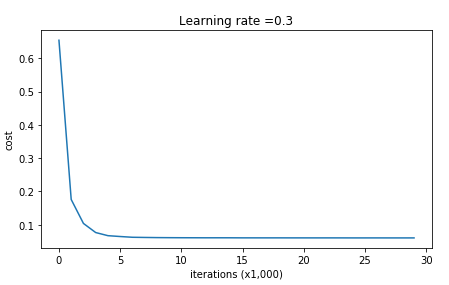
\includegraphics[scale=.51]{dropout_cost}	\end{center}
	\end{minipage}
	\begin{minipage}[c]{9cm}
	\begin{center} 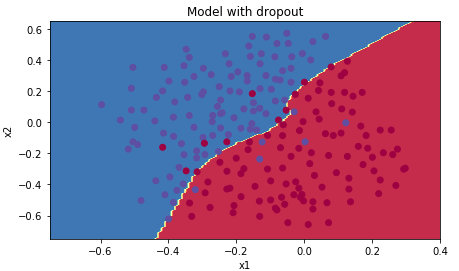
\includegraphics[scale=.51]{dropout_bound}	\end{center}
	\end{minipage} \vspace*{1.5mm} \newline
	As we can see, our model has increased its test accuracy by 5\% from the baseline by using dropout. Remeber that dropout is only used during training and never during testing. Our deep learning frameworks (such as TensorFlow) come with a dropout layer implementation that we will learn about in the future. \newpage
%%%% PAGE 45 %%%%

	\subsubsection{Programming Assignment (Gradient Checking)}
	\begin{lstlisting}
	# Packages
	import numpy as np
	from testCases import *
	from gc_utils import sigmoid, relu, dictionary_to_vector, vector_to_dictionary, 
	                     gradients_to_vector \end{lstlisting} \vspace*{1mm}
	Backpropagation computes the gradients $\frac{\partial J}{\partial \theta}$, where $\theta$ denotes the parameters of the model. $J$ is computed using forward propagation and your loss function. If you are confident that your forward propagation is correct and that your computing $J$ correctly, you can use your code for computing $J$ to verify the code for computing $\frac{\partial J}{\partial \theta}$. \vspace*{1mm} \\
	Let's look back at the definition of a derivative (or gradient):
	$$ \frac{\partial J}{\partial \theta} = \lim_{\varepsilon \to 0} \frac{J(\theta + \varepsilon) - J(\theta - \varepsilon)}{2 \varepsilon}$$
	We can use the above equation and a small value for $\varepsilon$ to check that your code for computing $\frac{\partial J}{\partial \theta}$ is correct. Remeber that we want our error to be equal to or smaller than our $\epsilon$ value. \\~\\
	Consider a \textbf{1D linear function} $J(\theta) = \theta x$. The model contains only a single real-valued parameter $\theta$, and takes $x$ as input. We will implement code to compute \textit{J} and its derivative. We will then use gradient checking to make sure our backward propagation is correct. \vspace*{1mm} \\
	\begin{center} 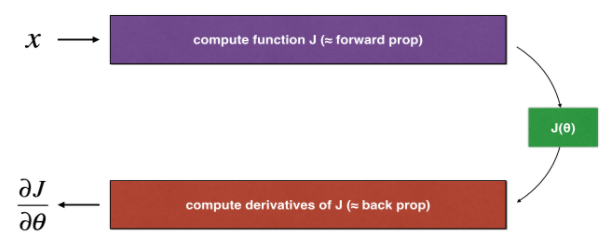
\includegraphics[scale=.5]{1d_grad_check} \\	\end{center}
	First start with $x$, then evaluate the function $J(x)$ (``forward propagation"). Then compute the derivative $\frac{\partial J}{\partial \theta}$ (``backward propagation"). 
	\begin{lstlisting}
	def forward_propagation(x, theta):
		"""
		Implement the linear forward propagation (J = theta * x)
		"""
		J = np.multiply(theta, x)		
		return J
	
	def backward_propagation(x, theta):
		"""
		Computes the derivative of J with respect to theta (dtheta = x).
		"""
		dtheta = x		
		return dtheta \end{lstlisting} \vspace*{1mm}
	Now we implement gradient checking to see if our back propagation function is working. We first compute \textit{gradapprox} by using the formula above and a small value for $\epsilon$. We follow these steps: \vspace*{1mm} \\
	\hspace*{3mm} 1. $\theta^{+} = \theta + \varepsilon$ \\
	\hspace*{3mm} 2. $\theta^{-} = \theta - \varepsilon$\\
	\hspace*{3mm} 3. $J^{+} = J(\theta^{+})$\\
	\hspace*{3mm} 4. $J^{-} = J(\theta^{-})$\\
	\hspace*{3mm} 5. $gradapprox = \frac{J^{+} - J^{-}}{2  \varepsilon}$ \newpage
%%%% PAGE 46 %%%%

	\noindent We then compute the gradient using backwards propagation and store it in variable \textit{grad}. Finally, we compute the difference with the following formula: $$ difference = \frac {\mid\mid grad - gradapprox \mid\mid_2}{\mid\mid grad \mid\mid_2 + \mid\mid gradapprox \mid\mid_2}$$ Note that If this difference is small (less than $\epsilon$), you can be quite confident that you have computed your gradient correctly. Otherwise, there may be a mistake in the gradient computation.       
	\begin{lstlisting}
	def gradient_check(x, theta, epsilon = 1e-7):
		"""
		Implement gradient checking for backward propagation.
		
		Arguments:
		x -- a real-valued input
		theta -- our parameter, a real number as well
		epsilon -- tiny shift to the input to compute approximated gradient with
		
		Returns:
		difference -- difference between the approx gradient and the back prop gradient
		"""
		# Compute gradapprox
		thetaplus = theta + epsilon # Step 1
		thetaminus = theta - epsilon # Step 2
		J_plus = forward_propagation(x, thetaplus) # Step 3
		J_minus = forward_propagation(x, thetaminus) # Step 4
		gradapprox = (J_plus - J_minus) / (2.*epsilon) # Step 5
		
		grad = backward_propagation(x, theta) # Compute gradient
		
		numerator = np.linalg.norm(grad-gradapprox) 
		denominator = np.linalg.norm(grad) + np.linalg.norm(gradapprox)
		difference = numerator/denominator                          
		
		if difference < 1e-7: # epsilon value
			print ("The gradient is correct!")
		else:
			print ("The gradient is wrong!")
		
		return difference \end{lstlisting} \vspace*{3mm}
	Now, we want to see how to implement \textbf{N-Dimensional} gradient checking. The following picture shows the forward and back propagation steps our model takes. \\
	\begin{center}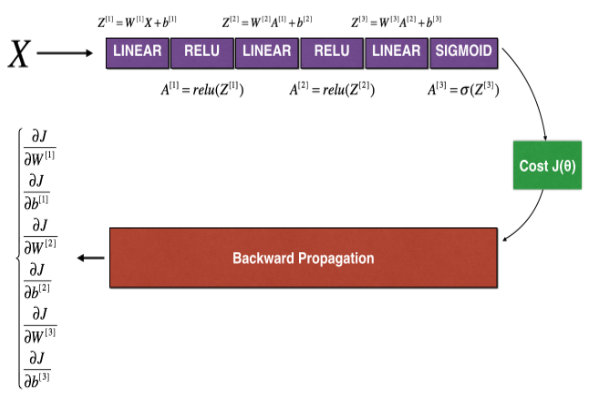
\includegraphics[scale=.65]{n_dim_grad_model} \end{center} \newpage
%%%% PAGE 47 %%%%

	\noindent Our forward and back propagation are already built for us, so lets take a look:
	\begin{lstlisting}
	def forward_propagation_n(X, Y, parameters):
		"""
		Arguments:
		X -- training set for m examples
		Y -- labels for m examples 
		parameters -- python dictionary containing your parameters
		"""
		# retrieve parameters
		m = X.shape[1]
		W1 = parameters["W1"]
		b1 = parameters["b1"]
		W2 = parameters["W2"]
		b2 = parameters["b2"]
		W3 = parameters["W3"]
		b3 = parameters["b3"]
		
		# LINEAR -> RELU -> LINEAR -> RELU -> LINEAR -> SIGMOID
		Z1 = np.dot(W1, X) + b1
		A1 = relu(Z1)
		Z2 = np.dot(W2, A1) + b2
		A2 = relu(Z2)
		Z3 = np.dot(W3, A2) + b3
		A3 = sigmoid(Z3)
		
		# Cost
		logprobs = np.multiply(-np.log(A3),Y) + np.multiply(-np.log(1 - A3), 1 - Y)
		cost = 1./m * np.sum(logprobs)
		
		cache = (Z1, A1, W1, b1, Z2, A2, W2, b2, Z3, A3, W3, b3)
		return cost, cache
	
	def backward_propagation_n(X, Y, cache):
		"""
		Arguments:
		X -- input datapoint, of shape (input size, 1)
		Y -- true "label"
		cache -- cache output from forward_propagation_n()
		"""
		m = X.shape[1]
		(Z1, A1, W1, b1, Z2, A2, W2, b2, Z3, A3, W3, b3) = cache
		
		dZ3 = A3 - Y
		dW3 = 1./m * np.dot(dZ3, A2.T)
		db3 = 1./m * np.sum(dZ3, axis=1, keepdims = True)
		
		dA2 = np.dot(W3.T, dZ3)
		dZ2 = np.multiply(dA2, np.int64(A2 > 0))
		dW2 = 1./m * np.dot(dZ2, A1.T)
		db2 = 1./m * np.sum(dZ2, axis=1, keepdims = True)
		
		dA1 = np.dot(W2.T, dZ2)
		dZ1 = np.multiply(dA1, np.int64(A1 > 0))
		dW1 = 1./m * np.dot(dZ1, X.T)
		db1 = 1./m * np.sum(dZ1, axis=1, keepdims = True)
		
		gradients = {"dZ3": dZ3, "dW3": dW3, "db3": db3,
		             "dA2": dA2, "dZ2": dZ2, "dW2": dW2, "db2": db2,
		             "dA1": dA1, "dZ1": dZ1, "dW1": dW1, "db1": db1}
		
		return gradients \end{lstlisting} \newpage
%%%% PAGE 48 %%%%

	\noindent We will use the same formula from above in order to find $\frac{\partial J}{\partial \theta}$. However, $\theta$ is not a scalar anymore. It is a dictionary called ``parameters". We implemented a function ``dictionary\_to\_vector()" for you. It converts the ``parameters" dictionary into a vector called ``values", obtained by reshaping all parameters (W1, b1, W2, b2, W3, b3) into vectors and concatenating them.	The inverse function is ``vector\_to\_dictionary" which outputs back the ``parameters" dictionary.
	\begin{lstlisting}
	def gradient_check_n(parameters, gradients, X, Y, epsilon = 1e-7):
		"""
		Arguments:
		parameters -- python dictionary containing your parameters 
		grad -- output of backward_propagation_n, contains gradients
		x -- input datapoint, of shape (input size, 1)
		y -- true "label"
		epsilon -- tiny shift to the input to compute approximated gradient with 
		"""
		# Set-up variables
		parameters_values, _ = dictionary_to_vector(parameters)
		grad = gradients_to_vector(gradients)
		num_parameters = parameters_values.shape[0]
		J_plus = np.zeros((num_parameters, 1))
		J_minus = np.zeros((num_parameters, 1))
		gradapprox = np.zeros((num_parameters, 1))
		
		# Compute gradapprox
		for i in range(num_parameters):
			
			# Compute J_plus[i]
			thetaplus = np.copy(parameters_values)                                    
			thetaplus[i][0] = thetaplus[i] + epsilon                               
			J_plus[i], _ = forward_propagation_n(X, Y, vector_to_dictionary(thetaplus))  

			
			# Compute J_minus[i]
			thetaminus = np.copy(parameters_values)                    
			thetaminus[i][0] = thetaminus[i] - epsilon         
			J_minus[i], _ = forward_propagation_n(X, Y, vector_to_dictionary(thetaminus)) 
			
			# Compute gradapprox[i]
			gradapprox[i] = (J_plus[i] - J_minus[i]) / (2.*epsilon)
		
		# Compare gradapprox to backward propagation gradients by computing difference.
		numerator = np.linalg.norm(grad-gradapprox)           
		denominator = np.linalg.norm(grad) + np.linalg.norm(gradapprox)      
		difference = numerator/denominator   
		
		if difference > 2e-7:
			print ("There is a mistake in the backward propagation! difference = " + 
			       str(difference))
		else:
			print ("Your backward propagation works perfectly fine! difference = " + 
			       str(difference))
		
		return difference\end{lstlisting} \vspace*{1mm}
	A few takeaways from this assignment: \\
	\hspace*{3mm} - Gradient Checking is slow! Approximating the gradient with $\frac{\partial J}{\partial \theta} \approx  \frac{J(\theta + \varepsilon) - J(\theta - \varepsilon)}{2 \varepsilon}$ is computationally \hspace*{6mm} costly. For this reason, we don't run gradient checking at every iteration during training. Just a \hspace*{6mm} few times to check if the gradient is correct. \\
	\hspace*{3mm} - The gradient checking we implemented doesn't work with dropout. You would usually run the \hspace*{6mm} gradient check algorithm without dropout to make sure your backprop is correct, then add dropout. \newpage
%%%% PAGE 49 %%%%

	\subsection{Optimization Algorithms}
	\subsubsection{Mini-Batch Gradient Descent}
	We will eventually start to train with datasets that have millions of training examples in them. In order to quickly train models, we want to split both the x and y datasets into \textbf{mini-batches}, in which we split our training data and their corresponding labels into equally small sizes. \vspace*{1mm} \\ Note that the notation to denote a mini batch will be $x^{\{t\}}$ and $y^{\{t\}}$, with shape $(n_x,\, batch\, size)$. \vspace*{2mm} \\
	To perform gradient descent using a mini batch, where our batch size (\textit{m}) will be 1,000. Mini-batch gradient descent performs must faster than a full batch and is the preferred method. The following represents 1 \textit{epoch} (one pass through the training set). Note that this is only one pass through the training set, we may want to put a loop around the for loop below in order to take multiple steps of gradient descent. \\~\\ for t=1, ..., num\_of\_batches
	\begin{center}
	Forward propagation on $x^{\{t\}}$ (vectorized implementation) \vspace*{1mm} \\
	Compute cost $J^{\{t\}} = \frac{1}{m} \sum_{i=1}^{l} L(\hat{y}^{(i)}, y^{(i)}) + regularization\; term $ \vspace*{1mm} \\
	Compute backpropagation for gradients using ($x^{\{t\}}$, $y^{\{t\}}$). \vspace*{1mm} \\
	Update parameters $W^{[l]}$ and $B^{[l]}$ \vspace*{1mm} \\
	\end{center}
	When training on mini-batches, if you plot $J^{\{t\}}$ it will be more noisy (not a smooth line) but still trends downwards. You also must choose a batch size that isn't too big or too small. If it is too big then it will take too long per iteration, but if it is too small then you loose speed from vectorization. Some guidelines to \textbf{choosing a batch size}: \\
	\hspace*{3mm} - If training set is under 2000, use batch gradient descent. \\
	\hspace*{3mm} - Typical mini-batch sizes are: 64, 128, 256, and 512. \\
	\hspace*{3mm} - Make sure that ($x^{\{t\}}$, $y^{\{t\}}$) fits in your CPU or GPU memory.
	\subsubsection{Exponentially Weighted Averages}
	There are algorithms that are faster than gradient descent, but in order to understand them we need to be able to use \textbf{exponentially weighted averages}. The will be a key component for our optimization algorithms, and we can use the following general formula: $$ V_t = \beta\,V_{t-1} + (1-\beta)\theta_t$$
	Note that the larger the $\beta$ value is, the more weight you are giving to the previous observation and the smooth your line will be (but it may also be slightly shifted). The smaller the $\beta$ value becomes, the less weight the previous observation has and the more noisy your line will be. \vspace*{1mm} \\
	We can use \textbf{bias correction} in order to compute these averages more accurately. To do this, we divide our values by (1-$\beta^t$). This gives us the general formula: $$ \frac{V_t}{1-\beta^t} = \frac{\beta\,V_{t-1} + (1-\beta)\theta_t}{1-\beta^t}$$
	We use this mainly in our ``initial" phase, where this new formula helps mostly in the beginning of our weighted average computations where \textit{t} is small. But as out \textit{t} grows larger, it will almost zero out the $\beta$ value and be similar to just dividing both sides by 1. \newpage
%%%% PAGE 50 %%%%

	\subsubsection{Gradient Descent with Momentum}
	In general, the \textbf{gradient descent with momentum} algorithm almost always works faster than standard gradient descent. The basic idea is to compute an exponentially weighted average of your gradients, and then use that gradient to update your weights instead. \vspace*{1mm} \\
	In general, we want our learning on the vertical axis to be slower in order to avoid oscillation (which leads to divergence in some cases).  We also want the horizontal axis to have faster learning so it moves towards to minimum. \vspace*{1mm} \\
	To implement momentum on a given iteration \textit{t}: \\
	\hspace*{3mm} - Compute dW, db on current mini-batch. \\
	\hspace*{3mm} - Compute $V_{dw} = \beta V_{dw} + (1-\beta)dW$ \\
	\hspace*{3mm} - Compute $V_{db} = \beta V_{db} + (1-\beta)db$ \\
	\hspace*{3mm} - Update parameters with: W = W - $\alpha V_{dw}$ \\
	\hspace*{50mm} b = b - $\alpha V_{db}$ \vspace*{1mm} \\
	We now have the hyperparameters $\alpha$ and $\beta$. Note that the most common value for $\beta$ = 0.9 (where we average over the last 10 gradients). We also initialize $V_{dw}$ = 0 and $V_{db}$ = 0. 
	\subsubsection{RMSprop}
	\textbf{RMSprop}, known as Root Mean Square prop, is another algorithm that can speed up gradient descent. The general idea is that RMSprop reduces the noise on the vertical axis when performing gradient descent, leading to a straighter line to the minimum value we want. \vspace*{1mm} \\
	To implement RMSprop on a given iteration \textit{t}: \\
	\hspace*{3mm} - Compute dW, db on current mini-batch. \\
	\hspace*{3mm} - Compute $S_{dw} = \beta_2 S_{dw} + (1-\beta_2)dW^2$ (note $dW^2$ is element wise square). \\
	\hspace*{3mm} - Compute $S_{db} = \beta_2 S_{db} + (1-\beta_2)db^2$ (note $db^2$ is element wise square).\\
	\hspace*{3mm} - Update parameters with: W = W - $\alpha \frac{dW}{\sqrt{S_{dw}+ \epsilon}}$ \\
	\hspace*{50mm} b = b - $\alpha \frac{db}{\sqrt{S_{db} + \epsilon}}$ \vspace*{1mm} \\
	Note that the $\epsilon$ that is added to the bottom of the fraction for updating the parameters is just a very small value to ensure that we do not divide by 0 when implementing the algorithm in code. 
	\subsubsection{Adam}
	The \textbf{Adam} (adaptive moment estimation) optimization algorithm takes the momentum and RMSprop algorithm and combines them. When implementing this, we initialize $V_{dw}$ = 0, $S_{dw}$ = 0, $V_{db}$ = 0, and $S_{db}$ = 0. Another important note is that the Adam optimizer uses bias correction. So on a given iteration \textit{t}: \\
	\hspace*{3mm} - Compute dW, db on current mini-batch. \\
	\hspace*{3mm} - Compute $V_{dw}$ and $V_{db}$ from \textit{momentum} algorithm. \\
	\hspace*{3mm} - Compute $S_{dw}$ and $S_{db}$ from \textit{RMSprop} algorithm. \\
	\hspace*{3mm} - Bias Correction: $V_{dw}^{corrected}$ = $\frac{V_{dw}}{(1-\beta^t_1)}$, $V_{db}^{corrected}$ = $\frac{V_{db}}{(1-\beta^t_1)}$ \\
	\hspace*{35mm} $S_{dw}^{corrected}$ = $\frac{S_{dw}}{(1-\beta^t_2)}$, $S_{dw}^{corrected}$ = $\frac{S_{dw}}{(1-\beta^t_2)}$ \\
	\hspace*{3mm} - Update parameters with: W = W - $\alpha \frac{V_{dw}^{corrected}}{\sqrt{S_{dw}^{corrected}+ \epsilon}}$ \\
	\hspace*{50mm} b = b - $\alpha \frac{V_{db}^{corrected}}{\sqrt{S_{db}^{corrected}+ \epsilon}}$ \vspace*{3mm} \\
	Common hyperparameter choices (recommended by creators of Adam): \\
	\hspace*{3mm} - $\alpha$ : needs to be tuned \\
	\hspace*{3mm} - $\beta_1$ : 0.9 \\
	\hspace*{3mm} - $\beta_1$ : 0.999 \\
	\hspace*{3mm} - $\epsilon$ : 10$^{-8}$ \newpage
%%%% PAGE 51 %%%%

	\subsubsection{Learning Rate Decay}
	One thing that might help to speed up your algorithm is to slowly reduce your learning rate over time, known as \textbf{learning rate decay}. This is useful because as learning converges, reducing the rate can help us take smaller steps and get closer to the minimum value we want. \vspace*{1mm} \\
	Remeber that 1 epoch = 1 pass through the dataset, so we can implement learning rate decay by: $$ \alpha = \frac{1}{1+ decay\_rate * num\_epoch}\; \alpha_0$$ 
	\subsubsection{Programming Assignment (Optimization)}
	Until now, we've always used Gradient Descent to update the parameters and minimize the cost. In this assignment, you will learn more advanced optimization methods that can speed up learning and perhaps even get you to a better final value for the cost function. Having a good optimization algorithm can be the difference between waiting days vs. just a few hours to get a good result. 
	\begin{lstlisting}
	import numpy as np
	import matplotlib.pyplot as plt
	import scipy.io
	import math
	import sklearn
	import sklearn.datasets
	
	from opt_utils_v1a import load_params_and_grads, initialize_parameters, 
	                          forward_propagation, backward_propagation
	from opt_utils_v1a import compute_cost, predict, predict_dec, plot_decision_boundary, 
	                          load_dataset
	from testCases import *	\end{lstlisting} \vspace*{1mm} 
	We will first implement \textbf{batch gradient descent parameter updating}, which is what we have been using previously. Recall that is rule is for layers 1 to L:
	$$ W^{[l]} = W^{[l]} - \alpha \text{ } dW^{[l]} $$
	$$ b^{[l]} = b^{[l]} - \alpha \text{ } db^{[l]} $$
	\begin{lstlisting}
	def update_parameters_with_gd(parameters, grads, learning_rate):
		"""
		Update parameters using one step of gradient descent
		
		Arguments:
		parameters -- python dictionary containing your parameters 
		grads -- python dictionary containing your gradients
		learning_rate -- the learning rate, scalar.
		
		Returns:
		parameters -- python dictionary containing your updated parameters 
		"""
		L = len(parameters) // 2 # number of layers in the neural networks
		
		# Update rule for each parameter
		for l in range(L):
			parameters["W" + str(l+1)] = parameters["W" + str(l+1)] - learning_rate * 
			                             grads["dW" + str(l+1)]
			parameters["b" + str(l+1)] = parameters["b" + str(l+1)] - learning_rate * 
			                             grads["db" + str(l+1)]
		
		return parameters \end{lstlisting} \newpage
%%%% PAGE 52 %%%%

	\noindent One variant of this is \textbf{Stochastic Gradient Descent} (SGD), which is equivalent to mini-batch gradient descent where each mini-batch has just 1 example. The update rule above does not change, but was does change is that we compute the gradient on just one example at a time and then updating the parameters. When the training set is large, SGD can be faster. But the parameters will ``oscillate" toward the minimum rather than converge smoothly.
	\begin{center}	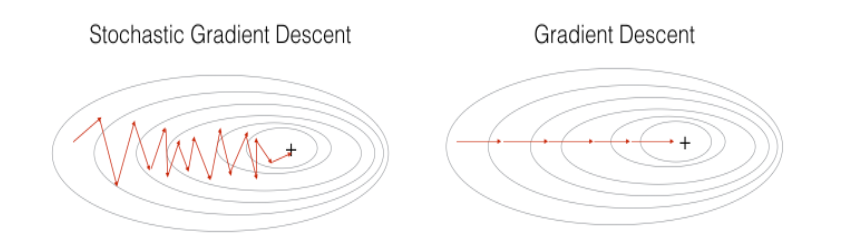
\includegraphics[scale=.6]{sgd_grad} \\	\end{center}
	Although SGD can be more efficient than batch gradient descent, you'll get better results if you use a batch-size in between the two. We call this \textbf{mini-batch gradient descent}, for which we loop over small batches of data and then update the parameters. An important note is that with all three of these, you will have to tune $\alpha$. 
	\begin{center}	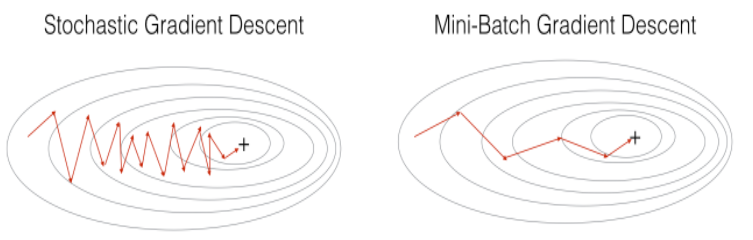
\includegraphics[scale=.6]{mini_grad} \\	\end{center}
	There are two steps in \textbf{building mini-batches} from the training set (X,Y): \vspace*{.7mm} \\
	\hspace*{3mm} 1) \textbf{Shuffle} - Create a shuffled version of the training set (X, Y) where each column of X and Y \hspace*{27mm} represents a training example. Note that this is done synchronously between X and Y \hspace*{27mm} such that after the shuffling, the $i^{th}$ column of X is the example corresponding to the $i^{th}$ \hspace*{27mm} label in Y. The shuffling step ensures that examples will be split randomly into different \hspace*{27mm} mini-batches. \vspace*{1.5mm} \\
	\hspace*{3mm} 2) \textbf{Partition} - Partition the shuffled (X, Y) into mini-batches of size \textit{mini\_batch\_size}. Note that the \hspace*{30mm} number of training examples is not always divisible \textit{by mini\_batch\_size}. The last mini \hspace*{30mm} batch might be smaller, but you don't need to worry about this. \\~\\
	Note that if the last mini-batch is smaller than the given batch size (in our case we will use 64), then we will round down the number of full mini batches to the nearest integer using math.floor(). This means for the total full mini-batches, we use: $$ math.floor(\frac{m}{mini\_batch\_size}) $$ This means that the final mini-batch, if not a full size, will be found by using: $$ m - mini\_batch\_size * math.floor(\frac{m}{mini\_batch\_size}) $$
	We will implement this idea in Python code, where we handle an end case when the last batch is not a full size.	\newpage
%%%% PAGE 53 %%%%

	\begin{lstlisting}
	def random_mini_batches(X, Y, mini_batch_size = 64, seed = 0):
		"""
		Creates a list of random minibatches from (X, Y)
		
		Arguments:
		X -- input data, of shape (input size, m)
		Y -- true "label" vector (1 for blue dot / 0 for red dot), of shape (1, m)
		mini_batch_size -- size of the mini-batches, integer
		
		Returns:
		mini_batches -- list of synchronous (mini_batch_X, mini_batch_Y)
		"""
		np.random.seed(seed) # To make your "random" minibatches the same as ours
		m = X.shape[1] # number of training examples
		mini_batches = []
		
		# Step 1: Shuffle (X, Y)
		permutation = list(np.random.permutation(m))
		shuffled_X = X[:, permutation]
		shuffled_Y = Y[:, permutation].reshape((1,m))
		
		# Step 2: Partition (shuffled_X, shuffled_Y). Minus the end case.
		num_complete_minibatches = math.floor(m/mini_batch_size) # round down
			for k in range(0, num_complete_minibatches):
			mini_batch_X = shuffled_X[:, k*mini_batch_size: (k+1)*mini_batch_size]
			mini_batch_Y = shuffled_Y[:, k*mini_batch_size: (k+1)*mini_batch_size]
			mini_batch = (mini_batch_X, mini_batch_Y)
			mini_batches.append(mini_batch)
		
		# Handling the end case (last mini-batch < mini_batch_size)
		if m % mini_batch_size != 0:
			mini_batch_X = shuffled_X[:, -(m-mini_batch_size*num_complete_minibatches):m]
			mini_batch_Y = shuffled_Y[:, -(m-mini_batch_size*num_complete_minibatches):m]
			mini_batch = (mini_batch_X, mini_batch_Y)
			mini_batches.append(mini_batch)
		
		return mini_batches \end{lstlisting} \vspace*{1mm}
	Because mini-batch gradient descent makes a parameter update after seeing just a subset of examples, the direction of the update has some variance, and so the path taken by mini-batch gradient descent will ``oscillate" toward convergence. Using momentum can reduce these oscillations. \textbf{Momentum} takes into account the past gradients to smooth out the update. We will store the `direction' of the previous gradients in the variable $v$. Formally, this will be the exponentially weighted average of the gradient on previous steps.
	\begin{center}	\includegraphics[scale=.6]{velocity} \\	\end{center}
	We will first \textbf{initialize the velocity}. It needs to be an array of zeros that are the same size as the parameters they will be applied on. Because they are zeros, the algorithm will take a few iterations to ``build up" velocity and start to take bigger steps. \newpage
%%%% PAGE 54 %%%%

	\begin{lstlisting}
	def initialize_velocity(parameters):
		"""
		Initializes the velocity as a python dictionary
		
		Arguments:
		parameters -- python dictionary containing your parameters.
		
		Returns:
		v -- python dictionary containing the velocity.

		"""
		L = len(parameters) // 2 # number of layers in the neural networks
		v = {}
		
		# Initialize velocity
		for l in range(L):
			v["dW" + str(l+1)] = np.zeros((parameters["W" + str(l+1)].shape))
			v["db" + str(l+1)] = np.zeros((parameters["b" + str(l+1)].shape))
		
		return v \end{lstlisting} \vspace*{1mm}
	Now that we have initialized our velocity, we want to implement the \textbf{parameters update with momentum}. The update rule is that for layers t to L: $$ \begin{cases}
	v_{dW^{[l]}} = \beta v_{dW^{[l]}} + (1 - \beta) dW^{[l]} \\
	W^{[l]} = W^{[l]} - \alpha v_{dW^{[l]}}
	\end{cases}$$	
	$$\begin{cases}
	v_{db^{[l]}} = \beta v_{db^{[l]}} + (1 - \beta) db^{[l]} \\
	b^{[l]} = b^{[l]} - \alpha v_{db^{[l]}} 
	\end{cases}$$
	where L is the number of layers, $\beta$ is the momentum and $\alpha$ is the learning rate. A common value for $\beta$ is between 0.8 to 0.999 (default is 0.9 if you don't feel like tuning it). 
	\begin{lstlisting}
	def update_parameters_with_momentum(parameters, grads, v, beta, learning_rate):
		"""
		Update parameters using Momentum
		
		Arguments:
		parameters -- python dictionary containing your parameters:
		grads -- python dictionary containing your gradients for each parameters:
		v -- python dictionary containing the current velocity:
		beta -- the momentum hyperparameter, scalar
		learning_rate -- the learning rate, scalar
		
		Returns:
		parameters -- python dictionary containing your updated parameters 
		v -- python dictionary containing your updated velocities
		"""
		L = len(parameters) // 2 # number of layers in the neural networks
		
		# Momentum update for each parameter
		for l in range(L):
			v["dW" + str(l+1)] = beta*v["dW" + str(l+1)] + (1-beta)*grads["dW" + str(l+1)]
			v["db" + str(l+1)] = beta*v["db" + str(l+1)] + (1-beta)*grads["db" + str(l+1)]
			parameters["W" + str(l+1)] = parameters["W" + str(l+1)] - 
			                             learning_rate*v["dW" + str(l+1)]
			parameters["b" + str(l+1)] = parameters["b" + str(l+1)] - 
			                             learning_rate*v["db" + str(l+1)]
	
		return parameters, v \end{lstlisting} \newpage
%%%% PAGE 55 %%%%

	\noindent \textbf{Adam} is one of the most effective optimization algorithms for training neural networks. It combines ideas from RMSprop and Momentum. The update rule for this is that for layers 1 to L:
	$$\begin{cases}
	v_{dW^{[l]}} = \beta_1 v_{dW^{[l]}} + (1 - \beta_1) \frac{\partial \mathcal{J} }{ \partial W^{[l]} } \\
	v^{corrected}_{dW^{[l]}} = \frac{v_{dW^{[l]}}}{1 - (\beta_1)^t} \\
	s_{dW^{[l]}} = \beta_2 s_{dW^{[l]}} + (1 - \beta_2) (\frac{\partial \mathcal{J} }{\partial W^{[l]} })^2 \\
	s^{corrected}_{dW^{[l]}} = \frac{s_{dW^{[l]}}}{1 - (\beta_2)^t} \\
	W^{[l]} = W^{[l]} - \alpha \frac{v^{corrected}_{dW^{[l]}}}{\sqrt{s^{corrected}_{dW^{[l]}}} + \varepsilon}
	\end{cases}$$ where: \\
	\hspace*{2mm} - t counts the number of steps taken of Adam \\
	\hspace*{2mm} - L is the number of layers\\
	\hspace*{2mm} - $\beta_1$ and $\beta_2$ are hyperparameters that control the two exponentially weighted averages. \\
	\hspace*{2mm} - $\alpha$ is the learning rate\\
	\hspace*{2mm} - $\varepsilon$ is a very small number to avoid dividing by zero \vspace*{1mm} \\
	We will first \textbf{initialize the Adam parameters}, which need to be arrays of zeros.
	\begin{lstlisting}
	def initialize_adam(parameters) :
		"""
		Initializes v and s as two python dictionaries
		
		Arguments:
		parameters -- python dictionary containing your parameters.
		
		Returns: 
		v -- dict that contains the exponentially weighted average of the gradient.
		s -- dict that contains the exponentially weighted average of the squared gradient.
		"""
		L = len(parameters) // 2 # number of layers in the neural networks
		v = {}
		s = {}
		
		# Initialize v, s.
		for l in range(L):
			v["dW" + str(l+1)] = np.zeros((parameters["W" + str(l+1)].shape))
			v["db" + str(l+1)] = np.zeros((parameters["b" + str(l+1)].shape))
			s["dW" + str(l+1)] = np.zeros((parameters["W" + str(l+1)].shape))
			s["db" + str(l+1)] = np.zeros((parameters["b" + str(l+1)].shape))
		
		return v, s	\end{lstlisting} \vspace*{1mm}
	Now we want to implement \textbf{parameter updating with Adam}. 
	\begin{lstlisting}
	def update_parameters_with_adam(parameters, grads, v, s, t, learning_rate = 0.01,
	                                beta1 = 0.9, beta2 = 0.999,  epsilon = 1e-8):
		"""
		Update parameters using Adam
		
		Arguments:
		parameters -- python dictionary containing your parameters:
		grads -- python dictionary containing your gradients for each parameters:
		v -- Adam variable, moving average of the first gradient, python dictionary
		s -- Adam variable, moving average of the squared gradient, python dictionary 
		learning_rate -- the learning rate, scalar.
		beta1 -- Exponential decay hyperparameter for the first moment estimates 
		beta2 -- Exponential decay hyperparameter for the second moment estimates 
		epsilon -- hyperparameter preventing division by zero in Adam updates \end{lstlisting} \newpage
%%%% PAGE 56 %%%%
		
		\begin{lstlisting}
		"""
		Returns:
		parameters -- python dictionary containing your updated parameters 
		v -- Adam variable, moving average of the first gradient, python dictionary
		s -- Adam variable, moving average of the squared gradient, python dictionary
		"""
		L = len(parameters) // 2 # number of layers in the neural networks
		v_corrected = {} # Initializing first moment estimate
		s_corrected = {} # Initializing second moment estimate
		
		# Perform Adam update on all parameters
		for l in range(L):
			# Moving average of the gradients
			v["dW" + str(l+1)] = beta1*v["dW" + str(l+1)] + (1-beta1)*grads["dW" + str(l+1)]
			v["db" + str(l+1)] = beta1*v["db" + str(l+1)] + (1-beta1)*grads["db" + str(l+1)]
			
			# Compute bias-corrected first moment estimate
			v_corrected["dW" + str(l+1)] = v["dW" + str(l+1)] / (1-np.power(beta1,t))
			v_corrected["db" + str(l+1)] = v["db" + str(l+1)] / (1-np.power(beta1,t))
			
			# Moving average of the squared gradients
			s["dW" + str(l+1)] = beta2*s["dW" + str(l+1)] + (1-beta2)*np.power(grads["dW" + 
			                                                                   str(l+1)], 2)
			s["db" + str(l+1)] = beta2*s["db" + str(l+1)] + (1-beta2)*np.power(grads["db" + 
			                                                                   str(l+1)], 2)
			
			# Compute bias-corrected second moment estimate
			s_corrected["dW" + str(l+1)] = s["dW" + str(l+1)] / (1-np.power(beta2,t))
			s_corrected["db" + str(l+1)] = s["db" + str(l+1)] / (1-np.power(beta2,t))
			
			# Update parameters
			parameters["W" + str(l+1)] = parameters["W" + str(l+1)] - learning_rate * 
			                             v_corrected["dW" + str(l+1)] / 
			                             np.sqrt(s_corrected["dW" + str(l+1)] + epsilon)
			parameters["b" + str(l+1)] = parameters["b" + str(l+1)] - learning_rate * 
			                             v_corrected["db" + str(l+1)] / 
			                             np.sqrt(s_corrected["db" + str(l+1)] + epsilon)
		return parameters, v, s \end{lstlisting} \vspace*{1mm}
	We now have three working optimization algorithms (mini-batch gradient descent, Momentum, Adam). Let's \textbf{implement a model} with each of these optimizers and observe the difference. Lets use the following ``moons" dataset to test the different optimization methods.
	\begin{center} \includegraphics[scale=.55]{moon_data} \\ \end{center}
	We have already implemented a 3-layer neural network. You will train it with: \\
	\hspace*{3mm} - \textit{Mini-batch Gradient Descent}: it will call your function: \\
	\hspace*{7mm} - update\_parameters\_with\_gd() \\
	\hspace*{3mm} - \textit{Mini-batch Momentum}: it will call your functions: \\
	\hspace*{7mm} - initialize\_velocity() and update\_parameters\_with\_momentum() \\
	\hspace*{3mm} - \textit{Mini-batch Adam}: it will call your functions: \\
	\hspace*{7mm} - initialize\_adam() and update\_parameters\_with\_adam() \newpage
%%%% PAGE 57 %%%%

	\begin{lstlisting}
	def model(X, Y, layers_dims, optimizer, learning_rate = 0.0007, mini_batch_size = 64, 
	          beta = 0.9, beta1 = 0.9, beta2 = 0.999,  epsilon = 1e-8, 
	          num_epochs = 10000, print_cost = True):
		"""
		3-layer neural network model which can be run in different optimizer modes.
		
		Arguments:
		X -- input data, of shape (2, m)
		Y -- true "label" vector (1 for blue dot / 0 for red dot), of shape (1, m)
		layers_dims -- python list, containing the size of each layer
		learning_rate -- the learning rate, scalar.
		mini_batch_size -- the size of a mini batch
		beta -- Momentum hyperparameter
		beta1 -- Exponential decay hyperparameter for the past gradients estimates 
		beta2 -- Exponential decay hyperparameter for the past squared gradients estimates 
		epsilon -- hyperparameter preventing division by zero in Adam updates
		num_epochs -- number of epochs
		print_cost -- True to print the cost every 1000 epochs
		
		Returns:
		parameters -- python dictionary containing your updated parameters 
		"""
		L = len(layers_dims) # number of layers in the neural networks
		costs = [] # to keep track of the cost
		t = 0 # initializing the counter required for Adam update
		seed = 10 
		m = X.shape[1] # number of training examples
		
		parameters = initialize_parameters(layers_dims) # Initialize parameters
		
		# Initialize the optimizer
		if optimizer == "gd":
			pass # no initialization required for gradient descent
		elif optimizer == "momentum":
			v = initialize_velocity(parameters)
		elif optimizer == "adam":
			v, s = initialize_adam(parameters)
		
		# Optimization loop
		for i in range(num_epochs):
			# Define the random minibatches.
			seed = seed + 1 # Increment seed to reshuffle differently after each epoch
			minibatches = random_mini_batches(X, Y, mini_batch_size, seed)
			cost_total = 0
			
			for minibatch in minibatches:
				(minibatch_X, minibatch_Y) = minibatch # Select a minibatch
				
				# Forward propagation
				a3, caches = forward_propagation(minibatch_X, parameters)
				
				# Compute cost and add to the cost total
				cost_total += compute_cost(a3, minibatch_Y)
				
				# Backward propagation
				grads = backward_propagation(minibatch_X, minibatch_Y, caches)
				
				# Update parameters
				if optimizer == "gd":
					parameters = update_parameters_with_gd(parameters, grads, learning_rate) \end{lstlisting} \newpage
%%%% PAGE 58 %%%%
					
	\begin{lstlisting}
				elif optimizer == "momentum":
					parameters, v = update_parameters_with_momentum(parameters, grads, v, beta, 
					                                                learning_rate)
				elif optimizer == "adam":
					t = t + 1 # Adam counter
					parameters, v, s = update_parameters_with_adam(parameters, grads, v, s, t, 
					                                               learning_rate, beta1, beta2,  
					                                               epsilon)
			cost_avg = cost_total / m
			
			# Print the cost every 1000 epoch
			if print_cost and i % 1000 == 0:
				print ("Cost after epoch %i: %f" %(i, cost_avg))
			if print_cost and i % 100 == 0:
				costs.append(cost_avg)
		
		# plot the cost
		plt.plot(costs)
		plt.ylabel('cost')
		plt.xlabel('epochs (per 100)')
		plt.title("Learning rate = " + str(learning_rate))
		plt.show()
		
		return parameters \end{lstlisting} \vspace*{1mm}
	We can now build a model with each of these optimizers.  
	\begin{lstlisting}
	# Mini-batch Gradient Descent
	layers_dims = [train_X.shape[0], 5, 2, 1]
	parameters = model(train_X, train_Y, layers_dims, optimizer = "gd")
	predictions1 = predict(train_X, train_Y, parameters)
	
	# Mini-batch Gradient Descent with Momentum
	layers_dims = [train_X.shape[0], 5, 2, 1]
	parameters = model(train_X, train_Y, layers_dims, beta = 0.9, optimizer = "momentum")
	predictions2 = predict(train_X, train_Y, parameters)
	
	# Mini-batch with Adam
	layers_dims = [train_X.shape[0], 5, 2, 1]
	parameters = model(train_X, train_Y, layers_dims, optimizer = "adam")
	predictions3 = predict(train_X, train_Y, parameters)	\end{lstlisting}
	\begin{center}
	\includegraphics[scale=.43]{opt_model_1} \hspace*{2mm} \includegraphics[scale=.43]{opt_model_2} \hspace*{2mm} \includegraphics[scale=.43]{opt_model_3} \\
	\end{center}
	The accuracies for the optimizers are as follows: Gradient Descent (79.7\%), Momentum (79.7\%), and Adam (94\%). \vspace*{1mm} \\
	Momentum usually helps, but given the small learning rate and the simplistic dataset, its impact is almost negligible. Also, the huge oscillations you see in the cost come from the fact that some mini-batches are more difficult than others for the optimization algorithm. \vspace*{1mm} \\
	Adam on the other hand, clearly outperforms mini-batch gradient descent and Momentum. If you run the model for more epochs on this simple dataset, all three methods will lead to very good results. However, you've seen that Adam converges a lot faster. \newpage
%%%% PAGE 59 %%%%

	\subsection{Hyperparameter Tuning, Batch Normalization, and Frameworks}
	\subsubsection{Tuning process}
	We have many options for \textbf{hyperparameter tuning} that can help to improve our model. Some of these could include $\alpha$, $\beta$, $n_h$, mini-batch size, and others. Note that the most important hyperparameter to tune is usually $\alpha$. \vspace*{1mm} \\
	When we are trying values, we want to make sure we are randomly selecting these hyperparameters value and not using a grid so that we can use more distinct value for each of the hyperparameters. Below is an example of how we would want to chose our values for two hyperparameters:  
	\begin{center} \includegraphics[scale=.15]{tuning_graph} \\ \end{center}
	Another method is called \textbf{coarse to find}, in which we find a group of values that work best with our model. From there, we ``zoom in" and create a box around the values that work best, and try more values in the neighboring range. \\~\\
	It is important to pick the appropriate \textbf{scale} on which to explore the hyperparameters. One example is choosing a value for $\alpha$ where we know that it should be between 0.0001 and 1. We want to sample uniformly, but we also don't want a majority of the samples to come from one side of the value range. To avoid this, we can use \textbf{log scaling}, for which we do the following: \vspace*{.5mm} \\
	\hspace*{3mm} - Compute a = log$_{10}$(min $\alpha$ value) \\
	\hspace*{3mm} - Compute b = log$_{10}$(max $\alpha$ value)\\
	\hspace*{3mm} - We now want to sample from 10$^a$ to 10$^b$\\
	\hspace*{3mm} - Set r = random value in range [a, b]\\
	\hspace*{3mm} - Set $\alpha$ = 10$^r$ \vspace*{1.5mm} \\
	Another tricky problem is tuning the value for $\beta$ used in exponentially weighted averages. Let say we expect $\beta$ to be between 0.9 and 0.999, then we can say that 1-$\beta$ is in the range 0.1 to 0.001. We then do the same steps as above, but set $\beta$ = 1 - 10$^r$. \\~\\
	There are two main ways that people perform hyperparameter tuning: \vspace*{.5mm} \\
	\hspace*{3mm} - \textbf{Babysitting One Model} : This is for when you don't have many computational resources (CPUs \hspace*{6mm} or GPUs) available to you. For training over multiple days, at the end of each day you change certain \hspace*{6mm} hyperparameters in our to decrease the cost function. \\
	\hspace*{3mm} - \textbf{Training Parallel Models} : This is when your train multiple models on the same problem, but \hspace*{6mm} with different hyperparameters. You then compare the results from each of them and pick the \hspace*{6mm} hyperparameters that performed best. This will be computationally expensive. 
	\subsubsection{Batch Normalization}
	We have seen previously that when we normalize our input features (X), our gradient descent works much smoother and our model is able to train faster. The question now is can we \textbf{normalize the activation} matrices in our deep Neural Network for each hidden layer (meaning normalize the input of a$^{[l-1]}$ for hidden layer \textit{l})? We will do this by normalizing Z$^{[l-1]}$. \newpage
%%%% PAGE 60 %%%%

	\noindent In order to \textbf{implement Batch Norm} for a given layer \textit{l}: \\
	\hspace*{3mm} - Given some intermediate values in the NN such as $z^{(1)},...,z^{(m)}$ \vspace*{.7mm}\\
	$$\mu = \frac{1}{m}\sum_i z^{(i)}$$
	$$\sigma^2 = \frac{1}{m}\sum_i (z^{(i)}-\mu)^2$$
	$$z^{(i)}_{norm} = \frac{z^{(i)}-\mu}{\sqrt{\sigma^2+\epsilon}}$$
	$$\tilde{z}^{(i)} = \gamma\, z^{(i)}_{norm} + \beta $$
	We don't always want the hidden units to have a mean = 0 and standard variance = 1. To avoid this, we compute $\tilde{z}$, where $\gamma$ and $\beta$ are learnable parameters of the model than can be updated. Note these parameters just let us set what we want the mean to be whatever we want it to be. For the later computations in our neural network, we now use $\tilde{z}^{(i)}$ instead of $z^{(i)}$ for a given layer \textit{l}. \\~\\
	When implementing batch norm with mini-batches, you use only the mini-batch data to calculate the batch norm parameters. Another important note is that when calculating $z^{[l]}$, we now drop the $b^{[l]}$ parameter and replace it with $\beta^{[l]}$. We do this because we want to normalize the data without increasing it by a value \textit{b}, and after we normalize we then add in $\beta$. Also, the shape of both $\beta^{[l]}$ and $\gamma^{[l]}$ will be ($n^{[l]}, 1$). \\~\\
	To implement \textbf{gradient descent with batch norm for mini-batches}, we create a for loop around the following steps for t=1 to num\_of\_mini\_batches: \vspace*{.5mm} \\
	\hspace*{3mm} - Compute forward propagation on $X^{\{t\}}$ \\
	\hspace*{7mm} - In each hidden layer, use BN to replace $z^{[l]}$ with $\tilde{z}^{[l]}$ \\
	\hspace*{3mm} - Use back propagation to compute $dW^{[l]}$, $d\beta^{[l]}$, $d\gamma^{[l]}$ (remember we drop \textit{b}). \\
	\hspace*{3mm} - Update parameters $W^{[l]}$, $\beta^{[l]}$, and $\gamma^{[l]}$ as usual. \vspace*{1mm} \\
	Note that in programming frameworks, you can usually implement batch norm with one line of code. \\~\\
	Batch norm processes our data one mini-batch at a time, but at \textbf{test time} we might need to process just one example at a time. Note that in the above equation, $\mu$ and $\sigma^2$ are computed for each mini-batch. However, during test time we need a different way to compute these values. We can do this by estimating using \textit{exponentially weighted averages across all mini-batches}. \vspace*{1mm} \\
	To explain further, we keep a running average of our $\mu$ and $\sigma^2$ values. When it is test time, we use these averages to compute the $z_{norm}$, which we then use to compute $\tilde{z}$ using our learned values for $\gamma$ and $\beta$: $$z_{norm} = \frac{z-\mu}{\sqrt{\sigma^2+\epsilon}} $$ $$\tilde{z} = \gamma\, z_{norm} + \beta $$ 
	\subsubsection{Multi-Class Classification (Softmax Regression)}
	\textbf{Softmax Regression} is a generalized version of Logistic Regression that allows use to classify \textit{C} classes instead of just a binary classification which we have previously focused on. The output layer for our Neural Network will have $n^{[L]}$ = C, where it matches the number of different classes we are trying to classify. This also means that $\hat{y}$ will have shape ($n^{[L]}$, 1). \newpage
%%%% PAGE 61 $$$$

	\noindent This model uses a \textbf{Softmax layer} for the output layer in order to generate these outputs. That means for layer \textit{L}, we compute $z^{[L]}$ as usual. But for the activation function, we do the following: $$ t = e^{(z^{[L]})} $$ $$ a^{[L]} = \frac{t}{\sum_{i=1} t_i} $$
	Above, \textit{t} is a temporary variable. We then divide this variables but the sum of all its values to \textit{normalize} the output. This will then result in a vector containing decimal outputs that represents probabilities, which has the shape (C,1). 
	\subsubsection{Programming Frameworks (TensorFlow)}
	IMPORTANT NOTE: This is in TensorFlow 1.0, so the syntax may be different with TensorFlow 2.0 \vspace*{2mm} \\
	Lets first take a look at how to \textbf{implement gradient descent} to minimize a cost function: $$ w^2 - 10w + 25 $$
	\begin{lstlisting}
	import numpy as np
	import tensorflow as tf
	
	w = tf.Variable(0, dtype=tf.float32) # define w
	cost = tf.add(tf.add(w**2, tf.multiply(-10.,w)), 25) # define cost function
	train = tf.train.GradientDescentOptimzer(0.01).minimize(cost)
	
	init = tf.global_variables_initializer() # standard code
	session = tf.Session() # create new session
	session.run(init) # initialize our variables
	
	for i in range(1000):
		session.run(train) # train the model
	print(session.run(w)) # 4.9999	\end{lstlisting} \vspace*{1mm}
	Above, we wanted to minimize the cost function so that it would equal 0. The ideal value for w is 5, and our code ended up at 4.9999. \vspace*{1mm} \\
	Lets now look at how to \textbf{read data} into TensorFlow and minimize the training data.
	\begin{lstlisting}
	coefficient = np.array([[1.], [-10.], [25.]]) # data to plug into x
	x = tf.placeholder(tf.float32, [3,1]) # think of as empty variables
	cost = x[0][0]*w**2 + x[1][0]*w + x[2][0]
	train = tf.train.GradientDescentOptimzer(0.01).minimize(cost)
	
	init = tf.global_variables_initializer() # standard code
	session = tf.Session() # create new session
	session.run(init) # initialize our variables
	
	for i in range(1000):
		session.run(train, feed_dict={x:coefficients}) # map x to our coefficients
	print(session.run(w)) # 4.9999 (same as above)	\end{lstlisting} \vspace*{1mm}
	Note that TensorFlow automatically implements back propagation when performing forward propagation, so we do not need to explicitly write code for this. \newpage
%%%% PAGE 62 %%%%

	\subsubsection{Programming Assignment (TensorFlow 1)}
	In this assignment, we will first go over an introduction to TensorFlow and writing code for the steps we have learned about Deep Networks. After this, we will then build a model to classify sign language numbers of a persons hand (numbers 0 to 5). \vspace*{2mm} \\
	Lets \textbf{import the packages} we will need for this assignment. 
	\begin{lstlisting}
	import math
	import numpy as np
	import h5py
	import matplotlib.pyplot as plt
	import tensorflow as tf
	from tensorflow.python.framework import ops
	from tf_utils import load_dataset, random_mini_batches, convert_to_one_hot, predict
	
	%matplotlib inline
	np.random.seed(1)\end{lstlisting} \vspace*{1mm}	
	Lets start by computing the following \textbf{Linear function}: $Y = WX + b$, where $W$ and $X$ are random matrices and b is a random vector. 
	\begin{lstlisting}
	def linear_function():		
		np.random.seed(1)
		
		X = tf.constant(np.random.randn(3,1), name='X')
		W = tf.constant(np.random.randn(4,3), name='W')
		b = tf.constant(np.random.randn(4,1), name='b')
		Y = tf.add(tf.matmul(W,X), b)
		
		# Create the session and run it on the variable you want to calculate
		sess = tf.Session()
		result = sess.run(Y)
		
		# close the session 
		sess.close()
		
		return result	\end{lstlisting} \vspace*{1mm}
	Now that we have our linear function, lets calculate the \textbf{Sigmoid}. Luckily, TensorFlow has built in Neural Network functions such as \textit{tf.sigmoid} and \textit{tf.softmax}.
	\begin{lstlisting}
	def sigmoid(z):
		"""
		Computes the sigmoid of z
		
		Arguments:
		z -- input value, scalar or vector
		"""
		# Create a placeholder for x
		x = tf.placeholder(tf.float32, name='x')
		
		# compute sigmoid(x)
		sigmoid = tf.sigmoid(x)
		
		# Create a session
		with tf.Session() as sess:
			# Run session and map z to x
			result = sess.run(sigmoid, feed_dict={x:z})
		
		return result \end{lstlisting} \newpage
%%%% PAGE 63 %%%%

	\noindent You can also use a built-in function to \textbf{compute the cost} of your neural network. So instead of needing to write code to compute this as a function of $a^{[2](i)}$ and $y^{(i)}$ for i=1...m: 
	$$ J = - \frac{1}{m}  \sum_{i = 1}^m  \large ( \small y^{(i)} \log a^{ [2] (i)} + (1-y^{(i)})\log (1-a^{ [2] (i)} )\large )\small$$
	you can do it in one line of code in TensorFlow. Note that the built in function will automatically compute the Sigmoid of z to get a.
	\begin{lstlisting}
	def cost(logits, labels):
		"""
		Computes the cost using the sigmoid cross entropy
		
		Arguments:
		logits -- vector containing z, output of the last linear unit 
		labels -- vector of labels y (1 or 0) 
		
		Note: logits will feed into z, and labels into y. 
		"""
		# Create the placeholders for "logits" (z) and "labels" (y)
		z = tf.placeholder(tf.float32, name='z')
		y = tf.placeholder(tf.float32, name='y')
		
		# Use the loss function
		cost = tf.nn.sigmoid_cross_entropy_with_logits(logits=z, labels=y)
		
		sess = tf.Session() # Create a session
		
		cost = sess.run(cost, feed_dict={z:logits, y:labels}) # Run the session
		
		sess.close() # Close the session
		
		return cost	\end{lstlisting} \vspace*{1mm}
	Many times in deep learning you will have a y vector with numbers ranging from 0 to C-1, where C is the number of classes. If C is for example 4, then you might have the following y vector which you will need to convert as follows:
	\begin{center} \includegraphics[scale=.6]{one_hot} \\	\end{center}
	This is called \textbf{one hot encoding}, because in the converted representation exactly one element of each column is ``hot" (meaning set to 1). In TensorFlow, we can do this with one line.
	\begin{lstlisting}
	def one_hot_matrix(labels, C):
		"""		
		Arguments:
		labels -- vector containing the labels 
		C -- number of classes, the depth of the one hot dimension
		"""
		C = tf.constant(C, name='C') # our 'depth'
		
		one_hot_matrix = tf.one_hot(labels, C, axis=0)

		sess = tf.Session()
		one_hot = sess.run(one_hot_matrix)
		sess.close()
		return one_hot # matrix of 0s and 1s	\end{lstlisting} \newpage
%%%% PAGE 64 %%%%

	\noindent Now we will \textbf{initialize a vector} of zeros and ones.
	\begin{lstlisting}
	def ones(shape):
		"""
		Arguments:
		shape -- shape of the array you want to create
		"""
		ones = tf.ones(shape)
		
		sess = tf.Session()
		ones = sess.run(ones)
		sess.close()
		
		return ones	\end{lstlisting} \vspace*{1mm}
	Now we will \textbf{build a Neural Network} using TensorFlow. Our problem statement is that we want to create a model that can turn sign language numbers pictures (valued 0 to 5) into regular numbers. \vspace*{.5mm} \\
	\hspace*{3mm} - Training set: 1080 pictures (64x64 pixels) of signs representing numbers (180 pictures per number). \\
	\hspace*{3mm} - Test set: 120 pictures (64x64 pixels) of signs representing numbers (20 pictures per number).
	\begin{center} \includegraphics[scale=.6]{sign_data}	\end{center}
	\begin{lstlisting}
	# Loading the dataset
	X_train_orig, Y_train_orig, X_test_orig, Y_test_orig, classes = load_dataset() \end{lstlisting} \vspace*{1mm}
	We want to \textbf{flatten the image} dataset, then \textbf{normalize} it by dividing by 255. On top of that, you will convert each label to a \textbf{one-hot} vector.
	\begin{lstlisting}
	# Flatten the training and test images
	X_train_flatten = X_train_orig.reshape(X_train_orig.shape[0], -1).T
	X_test_flatten = X_test_orig.reshape(X_test_orig.shape[0], -1).T
	# Normalize image vectors
	X_train = X_train_flatten/255. # shape (12288, 1080)
	X_test = X_test_flatten/255. # shape (6, 1080)
	# Convert training and test labels to one hot matrices
	Y_train = convert_to_one_hot(Y_train_orig, 6) # shape (6, 1080)
	Y_test = convert_to_one_hot(Y_test_orig, 6) # shape (6, 120)	\end{lstlisting} \vspace*{1mm}
	Note that 12288 comes from  64x64x3. Each image is square, 64 by 64 pixels, and 3 is for the RGB colors. Please make sure all these shapes make sense to you before continuing. \vspace*{1mm} \\
	The goal is to build an algorithm capable of recognizing a sign with high accuracy. To do so, you are going to build a TensorFlow model that is almost the same as one you have previously built in NumPy for cat recognition (but now using a softmax output). \vspace*{1mm} \\
	The model is LINEAR $\rightarrow$ RELU $\rightarrow$ LINEAR $\rightarrow$ RELU $\rightarrow$ LINEAR $\rightarrow$ SOFTMAX. The SIGMOID output layer has been converted to a SOFTMAX. A SOFTMAX layer generalizes SIGMOID to when there are more than two classes. \newpage
%%%% PAGE 65 %%%%

	\noindent The first task is to create \textbf{placeholders} for `X' and `Y'. This will allow you to later pass your training data in when you run your session. Note that $n_x$ is the size of an image vector (12288) and $n_y$ is the number of classes (6). We also use \textit{none} for the shape because it allows us to be more flexible with \textit{m}.
	\begin{lstlisting}
	def create_placeholders(n_x, n_y):
		X = tf.placeholder(tf.float32, [n_x, None], name='X')
		Y = tf.placeholder(tf.float32, [n_y, None], name='Y')
		
		return X, Y	\end{lstlisting} \vspace*{1mm}
	The second task is to \textbf{initialize the parameters}. You are going use Xavier Initialization for weights and Zero Initialization for biases. The shapes are given to us.
	\begin{lstlisting}
	def initialize_parameters():
		tf.set_random_seed(1) # so that your "random" numbers match ours
		
		W1 = tf.get_variable("W1", [25,12288], initializer = tf.contrib.layers.
		                                                     xavier_initializer(seed = 1))
		b1 = tf.get_variable("b1", [25,1], initializer = tf.zeros_initializer())
		W2 = tf.get_variable("W2", [12,25], initializer = tf.contrib.layers.
		                                                  xavier_initializer(seed = 1))
		b2 = tf.get_variable("b2", [12,1], initializer = tf.zeros_initializer())
		W3 = tf.get_variable("W3", [6,12], initializer = tf.contrib.layers.
		                                                 xavier_initializer(seed = 1))
		b3 = tf.get_variable("b3", [6,1], initializer = tf.zeros_initializer())
		
		parameters = {"W1": W1,	"b1": b1, "W2": W2,
		              "b2": b2, "W3": W3, "b3": b3}
	
		return parameters \end{lstlisting} \vspace*{1mm}
	We will now implement the \textbf{forward propagation} module. It is important to note that the forward propagation stops at `z3'. The reason is that in TensorFlow the last linear layer output is given as input to the function computing the loss. Note that we do not output any \textit{cache}, we will see why during back propagation.
	\begin{lstlisting}
	def forward_propagation(X, parameters):
		"""
		Implements: LINEAR -> RELU -> LINEAR -> RELU -> LINEAR -> SOFTMAX
		
		Arguments:
		X -- input dataset placeholder, of shape (input size, m)
		parameters -- python dictionary containing your parameters 
		
		Returns:
		Z3 -- the output of the last LINEAR unit (used for softmax)
		"""
		W1 = parameters['W1']
		b1 = parameters['b1']
		W2 = parameters['W2']
		b2 = parameters['b2']
		W3 = parameters['W3']
		b3 = parameters['b3']
		
		Z1 = tf.add(tf.matmul(W1, X), b1) 
		A1 = tf.nn.relu(Z1) 
		Z2 = tf.add(tf.matmul(W2, A1), b2)
		A2 = tf.nn.relu(Z2) 
		Z3 = tf.add(tf.matmul(W3, A2), b3) 

		return Z3 \end{lstlisting} \newpage
%%%% PAGE 66 %%%%

	\noindent Now it is time to \textbf{compute the cost}. Note that `logits' and `labels' are expected to have the shape (number of examples, number of classes), so that is why we transpose them below.
	\begin{lstlisting}
	def compute_cost(Z3, Y):
		"""
		Computes the cost
		
		Arguments:
		Z3 -- output of forward prop (the last LINEAR unit), of shape (6, m)
		Y -- "true" labels vector placeholder, same shape as Z3
		
		Returns:
		cost - Tensor of the cost function
		"""
		# fit the requirement for cost computation 
		logits = tf.transpose(Z3)
		labels = tf.transpose(Y)
		
		cost = tf.reduce_mean(tf.nn.softmax_cross_entropy_with_logits(logits=logits, 
		                                                              labels=labels))
		return cost	\end{lstlisting} \vspace*{1mm}
	Unlike before, frameworks handle all the \textbf{backpropagation} and the \textbf{parameters update} in 1 line of code. It is very easy to incorporate this line in the model. After you compute the cost function, you will create an \textit{optimizer} object. You have to call this object along with the cost when running the tf.session. When called, it will perform an optimization on the given cost with the chosen method and learning rate. One example of how to do this would be: 
	\begin{lstlisting}
	optimizer = tf.train.GradientDescentOptimizer(learning_rate = learning_rate).
	            minimize(cost)
	_ , c = sess.run([optimizer, cost], feed_dict={X: minibatch_X, Y: minibatch_Y})	\end{lstlisting} \vspace*{1mm}
	Now we will \textbf{build a model} using these functions and our training data.
	\begin{lstlisting}
	def model(X_train, Y_train, X_test, Y_test, learning_rate = 0.0001,
	          num_epochs = 1500, minibatch_size = 32, print_cost = True):
		"""
		Implements a 3-layer tensorflow NN: LINEAR->RELU->LINEAR->RELU->LINEAR->SOFTMAX.
		
		Arguments:
		X_train -- training set (input size = 12288, number of training examples = 1080)
		Y_train -- test set (output size = 6, number of training examples = 1080)
		X_test -- training set (input size = 12288, number of training examples = 120)
		Y_test -- test set (output size = 6, number of test examples = 120)
		learning_rate -- learning rate of the optimization
		num_epochs -- number of epochs of the optimization loop
		minibatch_size -- size of a minibatch
		print_cost -- True to print the cost every 100 epochs
		
		Returns:
		parameters -- parameters learnt by the model. They can then be used to predict.
		"""
		
		ops.reset_default_graph() # able to rerun the model without overwriting tf variables
		tf.set_random_seed(1) # to keep consistent results
		seed = 3 # to keep consistent results
		(n_x, m) = X_train.shape # (n_x: input size, m : number of examples in the train set)
		n_y = Y_train.shape[0] # n_y : output size
		costs = [] # To keep track of the cost \end{lstlisting} \newpage
%%%% PAGE 67 %%%%

	\begin{lstlisting}
		X, Y = create_placeholders(n_x, n_y) # Create Placeholders

		parameters = initialize_parameters() # Initialize parameters

		Z3 = forward_propagation(X, parameters) # Build the forward prop in the tf graph

		cost = compute_cost(Z3, Y) # Add cost function to tensorflow graph
		
		# Backpropagation: Define the tensorflow optimizer
		optimizer = tf.train.AdamOptimizer(learning_rate).minimize(cost)
		
		init = tf.global_variables_initializer() # Initialize all the variables
		
		with tf.Session() as sess: # Start the session to compute the tensorflow graph
			sess.run(init) # Run the initialization
			for epoch in range(num_epochs): # Do the training loop
				epoch_cost = 0. # Defines a cost related to an epoch
				num_minibatches = int(m / minibatch_size) # number of minibatches
				seed = seed + 1
				minibatches = random_mini_batches(X_train, Y_train, minibatch_size, seed)
				
				for minibatch in minibatches:
					(minibatch_X, minibatch_Y) = minibatch # Select a minibatch

					# Run the session to execute the "optimizer" and the "cost"
					_ , minibatch_cost = sess.run([optimizer, cost], feed_dict={X:minibatch_X, 
					                                                            Y:minibatch_Y})
					epoch_cost += minibatch_cost / minibatch_size
				
				# Print the cost every epoch
				if print_cost == True and epoch % 100 == 0:
					print ("Cost after epoch %i: %f" % (epoch, epoch_cost))
				if print_cost == True and epoch % 5 == 0:
					costs.append(epoch_cost)
		
			# plot the cost
			plt.plot(np.squeeze(costs))
			plt.ylabel('cost')
			plt.xlabel('iterations (per fives)')
			plt.title("Learning rate =" + str(learning_rate))
			plt.show()
			
			# lets save the parameters in a variable
			parameters = sess.run(parameters)
			print("Parameters have been trained!")
			
			# Calculate the correct predictions
			correct_prediction = tf.equal(tf.argmax(Z3), tf.argmax(Y))
			
			# Calculate accuracy on the test set
			accuracy = tf.reduce_mean(tf.cast(correct_prediction, "float"))
			
			print("Train Accuracy:", accuracy.eval({X: X_train, Y: Y_train}))
			print("Test Accuracy:", accuracy.eval({X: X_test, Y: Y_test}))
			
			return parameters \end{lstlisting} \vspace*{1mm} 
	Our model resulted in a 99.9\% train accuracy, and a 71.7\% test accuracy. Overall, our model seems big enough to fit the data well, but given the difference between the train and test set, we could try adding in L2 or dropout regularization to reduce overfitting. Each time we run the session on a mini-batch, it trains the parameters and will eventually obtained the best parameters we could find. \newpage
%%%% PAGE 68 %%%%

	\section{Structuring Machine Learning Projects}
	\subsection{Machine Learning Strategy 1}
	The chain of assumptions are: \vspace*{.5mm} \\
	\hspace*{3mm} 1) Fit training set well on cost function $\rightarrow$ tune by bigger network / different optimizer. \\
	\hspace*{3mm} 2) Fit dev set well on cost function $\rightarrow$ tune by regularization / bigger training set. \\
	\hspace*{3mm} 3) Fit test set well on cost function $\rightarrow$ tune with a bigger dev set. \\
	\hspace*{3mm} 4) Performs well in real world $\rightarrow$ tune by changing dev set or cost function.
	\subsubsection{Evaluation Metrics}
	If we are hyperparameter tuning or trying new algorithms, our progress will be much faster if you have a single real number evaluation metric that lets us quickly tell if the new thing we just tried is working better or worse than your last idea. It's a good idea to have a \textbf{single number evaluation metric} to do this. \vspace*{1.5mm} \\
	\textbf{Precision} - Of examples recognized as a certain class, the percentage that are correctly classified. \\
	\textbf{Recall} - The percentage of actual class member that  are correctly recognized. \\
	\textbf{F1 Score} - The average of precision and recall (best metric to use when comparing classifiers). \vspace*{1.5mm} \\
	Having a well defined dev set along with a single number evaluation metric allows us to tell which classifier is better. This can help us speed up the tuning our of model. \\~\\
	Another way we can choose which model we want to use after training is by using a \textbf{optimizing metric} and \textbf{satisficing metric}. For example, say we want to choose our model where we maximize accuracy subject to run time being less than a certain value. This means that accuracy is our \textit{optimizing metric}, while run time is our \textit{satisficing metric}. \vspace*{.5mm} \\
	In general, lets say we have N metrics we are observing for a given model. Then we want to choose 1 optimizing metric and N-1 satisficing metrics.
	
	\subsubsection{Setting up the Dev and Test sets}
	We want to make sure that our dev set and test set both come from the \textbf{same distribution}. Lets say that our data comes from many different regions (US, UK, China, etc.). Instead of choosing certain regions for each set, we want to \textit{randomly shuffle} all of the data into dev/test sets to make sure that it is distributed as evenly as possible. \vspace*{1mm} \\
	The general guideline is to choose a dev set and test set to reflect data you expect to get in the future and consider important to do well on. You don't want to train your model to do one thing, only to then use it to try and predict something else. \\~\\
	We often work with very large datasets (millions of observations). When it comes to \textbf{splitting the data}, it could be enough to do a 98\%, 1\%, 1\% split. For example, if we had 1,000,000 observations, then this split would give us 10,000 observations in both the dev and test sets. The size of the test set should be big enough to give high confidence in the overall performance of your system.  \vspace*{2mm} \\
	One note is that after deploying you model, if it allows users to use their own pictures, they might not be as high quality as the ones in the training/dev sets. If this is the case, you may want to add some of these more `low quality' pictures into your sets in order to prepare your model. \newpage
%%%% PAGE 69 %%%%

	\subsubsection{Comparing to Human-Level Performance}
	Over time, our model can increase its accuracy to beyond human-level. However, this will eventually slow down and begin to level off. Ideally, we want our model to reach \textbf{Bayes optimal error}, or the best possible error, meaning that no function that computes x$\rightarrow$y will perform better. This does not need to be 100\% accuracy (it is normal to have some type of error) which can be cause by low quality pictures, audio, video, etc. \vspace*{1.5mm} \\
	One reason that the model begins to slow down after passing human-level performance is because the difference between Bayes optimal error and human error is very close for many deep learning problems (image classification, audio, etc.). Another reason is because there are many tools that can help us surpass human-level performance such as: \vspace*{.5mm} \\
	\hspace*{3mm} - Get more labeled data from humans. \\
	\hspace*{3mm} - Gain insight from manual error analysis. \\
	\hspace*{3mm} - Better analysis of bias/variance. \\~\\
	We want our learning algorithm to do well on the data sets, but not too well. We can use \textbf{human-level error}, which we will consider very close to Bayes error and use as a proxy, to gauge where we want our model training/dev error to be near. \vspace*{1mm} \\
	\hspace*{3mm} - \textbf{Avoidable bias} : the difference between human (Bayes) error and the training error. \\
	\hspace*{3mm} - \textbf{Variance} : the difference between training and dev error. \vspace*{1mm} \\
	If our human error is much lower than the training/dev error, we will focus on reducing the avoidable bias. If our human error is very close to the training/dev error, we will focus on variance reduction. \\~\\
	The two fundamental assumptions of supervised learning: \\
	\hspace*{3mm} 1) You can fit the training set pretty well (achieve low \textit{avoidable bias}). \\
	\hspace*{3mm} 2) The training set performance generalizes pretty well to the dev/test set (achieve low \textit{variance}). \vspace*{2mm}\\
	We can reduce the following by: \\
	\hspace*{3mm} 1) Avoidable bias - bigger model, optimization algorithms, different NN architecture/hyperparameters. \\
	\hspace*{3mm} 2) Variance - more data, regularization, different NN architecture/hyperparameters.
	
	\subsection{Machine Learning Strategy 2}
	\subsubsection{Error Analysis}
	During \textbf{error analysis}, for example using a cat classifier, we are looking at images in our dev set that are mislabeled (incorrectly predicted). We want to look at the false positives and false negatives. One idea is manual error analysis, where we could chose 100 mislabeled dev set examples and see where we are making an error. \vspace*{1mm} \\
	Say we are using our cat classifier on dogs as well. We can create a spreadsheet for the 100 images we selected to help us fix dogs being classified as cats, fix images being misrecognized, and improve performance on blurry images. We can put each of these in a column with rows being the corresponding 100 pictures, and then total each column to find where our model is making the greatest error and where to improve. \\~\\
	If we have \textbf{incorrectly labeled examples} in our training data, we must look at the type of error. Deep learning algorithms are robust to \textit{random errors}, so if the number of mislabeled data is very small and the data set is very large, it is usually okay to leave the mislabeled data in the training set. However, if it is a \textit{systematic error} (such as all white dogs are labeled as cats), then it will need to be fixed. \newpage
%%%% PAGE 70 %%%%

	\noindent If we have mislabeled data in the dev set, we want to look at the overall dev set error. In this error, we want to see what percentage of these errors are from incorrect labels, and then errors due to other causes. If the error from incorrect labels is much smaller than errors from other causes, we want to focus on the bigger error that we can reduce to increase our accuracy. Some guidelines: \vspace*{.5mm} \\
	\hspace*{3mm} - Apply same process to your dev and test sets to make sure they come from same distribution. \\
	\hspace*{3mm} - Consider examining examples your algorithm got right as well as ones it got wrong (reduce bias). \\
	\hspace*{3mm} - Train and dev/test data may now come from different distributions (this is okay). \\~\\
	One method to speed up the process of improving a model is to build your first system quickly and then iterate. This means set up your dev/test set and metric, build your initial system quickly, and then use Bias/Variance analysis and Error analysis to prioritize the next steps. 	
	\subsubsection{Mismatched Data Distributions}
	We often want to train our models on as much data as possible, but we also want it all to come from the same distribution. For example, if we were building a cat classifier and we had 200,000 professional images from webpages and 10,000 images from a mobile app (which are blurry and not professional), instead of shuffling we would want to evenly distribute the mobile app images. So we can have all 200,000 web images in the training set along with 5,000 images from the mobile app. Then in our test/dev set, it will contain 5,000 mobile app images since this is what our model will be using when we deploy it. \\~\\
	Estimating bias and variance helps you prioritize what to work on next, but the way we analyze bias and variance changes when our training set comes from a different distribution than the dev/test sets. For example, our cat classifier that uses professional training images and mobile app dev images, the difference between the training error and dev error is because the data is different. \vspace*{1.5mm}\\ 
	To avoid this, we set up a \textbf{training-dev set}, which has the same distribution as the training set, but not used for training. Lets say we have the following error values: \\
	\hspace*{3mm} - Training error : 1\% \\
	\hspace*{3mm} - Training-dev error : 9\%\\
	\hspace*{3mm} - Dev error : 10\%\\
	This means we have a variance problem, because the model is not generalizing well on the training data (since we see it is performing well on the dev data). However, if the difference between the training-dev and dev error is higher, that means we have a \textit{data mismatch} problem. \vspace*{2mm} \\
	To judge bias/variance on mismatched training and dev/test sets, we look at: \vspace*{.5mm} \\
	\hspace*{3mm} - The difference between human level error and training set error, \textbf{avoidable bias}. \\
	\hspace*{3mm} - The difference between training set error and training-dev error, the \textbf{variance}. \\
	\hspace*{3mm} - The difference between training-dev error and dev error, the \textbf{data mismatch}. \\
	\hspace*{3mm} - The difference between dev error and test error, the \textbf{degree of overfitting to dev set}. \\~\\
	There is no exact method that we can use to improve our error between the training-dev error and the dev error. However, if you perform error analysis and find that you have a \textbf{data mismatch} problem, we can try: \\
	\hspace*{3mm} - Carry out manual error analysis to try to understand difference between training and dev/test sets.\\
	\hspace*{3mm} - Make training data more similar, or collect more data similar to dev/test sets. \vspace*{1.5mm} \\
	One method we can use is \textbf{artificial data synthesis}, where we combine multiple pieces of data to create one that we want. For example, if we have an audio clip of someone speaking and an audio clip of car noise, we can combine these two in order to synthesize in-car audio. Be cautious that you are now synthesizing data from just a small subset of the space of all possible examples. \newpage
%%%% PAGE 71 %%%%

	\subsubsection{Learning from Multiple Tasks}
	Sometimes you can take knowledge the neural network has learned from one task and apply that knowledge to a separate task, this is called \textbf{transfer learning}. If it is a small data set, we just retrain the last layer along with $W^{[L]}$ and $b^{[L]}$, then use this new output layer to make predictions on whatever our model does. If we have a large data set, we can retrain all the parameters in the Neural Network. The training from the old model becomes known as \textit{pre-training} and the parameters change we make from retraining is known as \textit{fine-tuning}. We can also add new layers to a Neural Network that has always been created if we want. \vspace*{1.5mm}\\ 
	We use transfer learning when we have a lot of data we are transferring from (the already built model) and less data for the model we are transferring to. We also want to make sure both models have the same input (images, audio, etc.). We also use transfer learning when we think low level features from A (early nodes in the network) will be helpful for the new model. \\~\\
	In \textbf{multi-task learning}, you start off simultaneously, trying to have one neural network do several things at the same time. And then each of these task helps hopefully all of the other task. For example, if we train a Neural Network for autonomous cars, we may want our model to be able to recognize multiple objects in an image. This means our output wont just be one label, but can be multiple labels that are all solved at the same time. It makes sense to use this when: \vspace*{.5mm} \\
	\hspace*{3mm} - Training on a set of tasks that could benefit from having shared lower-level features. \\
	\hspace*{3mm} - Usually: Amount of data you have for each task is quite similar. \\
	\hspace*{3mm} - Can train a big enough neural network to do well on all the tasks.
	
	
	\subsubsection{End-to-End Deep Learning}
	\textbf{End-to-end} deep learning trains a large Neural Network that goes from input to output, without all the steps in between. However, to do this you need a very large amount of data. \vspace*{2mm} \\
	Benefits for end-to-end learning: \\
	\hspace*{3mm} - Let the data speak. \\
	\hspace*{3mm} - Less hand-designing of components needed. \vspace*{1mm} \\
	Disadvantages for end-to-end learning: \\
	\hspace*{3mm} - May need a large amount of data. \\
	\hspace*{3mm} - Excludes potentially useful hand-designed components. \vspace*{2mm} \\
	When applying end-to-end deep learning, we want to ask ourselves if we have sufficient data to learn a function of the complexity needed to map x to y. \newpage
%%%% PAGE 72 %%%%

	\section{Convolutional Neural Networks}
	\subsection{Foundations of Convolutional Neural Networks}
	\subsubsection{Edge Detection}
	\begin{center}
	$\begin{bmatrix}
	3 & 0 & 1 & 2 & 7 & 4 \\ 1 & 5 & 8 & 9 & 3 & 1 \\ 2 & 7 & 2 & 5 & 1 & 3 \\ 0 & 1 & 3 & 1 & 7 & 8 \\ 4 & 2 & 1 & 6 & 2 & 8 \\ 2 & 4 & 5 & 2 & 3 & 9\end{bmatrix} $ $*$ $\begin{bmatrix} 1 & 0 & -1 \\ 1 & 0 & -1 \\ 1 & 0 & -1 \end{bmatrix}$ = $ \begin{bmatrix}
	-5 & -4 & 0 & 8 \\ -10 & -2 & 2 & 3 \\ 0 & -2 & -4 & -7 \\ -3 & -2 & -3 & -16 \end{bmatrix}$
	\end{center}
	For \textbf{vertical edge detection}, say we have a 6x6 greyscale image. To detect edges, we construct a 3x3 matrix (know as a ``filter" or ``kernel"). We then \textit{convolve} (denoted by $*$) the greyscale image with the filter, which will then result in a 4x4 matrix. To perform \textit{convolution} think of laying the 3x3 filter on top of the 6x6 (starting in the top left corner) and multiplying the values by the filter values, then adding all of them up. We then shift to the right by one and do the same process to get the next value in our 4x4 matrix. After we finish the row, we shift down one and repeat the process until our 4x4 matrix if filled. Below is an example of how this works:
	\begin{center}
	\includegraphics[scale=.5]{edge_dect}
	\end{center}
	For our greyscale vertical edge detection above, we say that there is an edge in a 3x3 region where there are bright pixels on the left (higher values) and dark pixels on the right (lower values). Note that we are not worried about the middle values. \\~\\
	We can also perform \textbf{horizontal edge detection}. For our example, a horizontal edge will be a 3x3 region where the pixels are bright on top and relatively dark on the bottom.
	\begin{center}
	\includegraphics[scale=.5]{horizontal} \includegraphics[scale=.5]{horizontal_2}	
	\end{center}
	When choosing our filter, there are many different options we can chose. We could use the ones above, a Sobel filter, Scharr filter, etc. One idea however is to learn the parameters using backpropagation, which will allow the model to find the best fit (could be one of the filters listed above or a custom one). This will also allow your model to possibly detect edges at any that aren't just horizontal and vertical, but also in between. $$ \begin{bmatrix}
	w_1 & w_2 & w_3 \\ w_4 & w_5 & w_6 \\ w_7 & w_8 & w_9 \end{bmatrix} $$ \newpage
%%%% PAGE 73 %%%%

	\subsubsection{Padding and Strides}
	In general we say that the image dimensions are ($n$ x $n$), filter dimensions are ($f$ x $f$), and our output dimensions are (($n-f+1$) x ($n-f+1$)). One problem with this is that we are shrinking the output, leading to throwing away information from edge. \vspace*{1mm}\\
	One way to avoid this is by \textbf{padding} the image with an additional border of one pixel around the entire matrix. For example, padding our 6x6 image will turn it into an 8x8 image. We let $p$ be our padding (in this case p=1), and our new output shape will be (($n+2p-f+1$) x ($n+2p-f+1$)). \vspace*{2mm} \\
	\textbf{Valid convolutions} - no padding, ($n$ x $n$) $*$ ($f$ x $f$) = (($n-f+1$) x ($n-f+1$)) \\
	\textbf{Same convolutions} - Pad so output matches input, where we want $p = \frac{f-1}{2}$. ($f$ is usually odd). \\~\\
	We can perform \textbf{strided convolution} by setting a stride value ($s$) and using that as our shift amount. For example, if s=2, then we shift to the right by 2 every time we perform convolution and shift down by 2 every time we start a new row. \vspace*{1mm}\\
	This means our new output has dimensions (($\frac{n+2p-f}{s}+1$) x ($\frac{n+2p-f}{s}+1$)). Note that we round down the fraction if it is not a whole number (take the \textit{floor} value). This is because if any of the filter box hangs outside of the image (+ padding region), then we do not compute the convolution value.
	
	\subsubsection{RGB Image Convolution}
	We can also perform edge detection on images that aren't just greyscale but also have color. We have the following: \\
	\hspace*{3mm} - Image: dimensions = (height x width x number of channels) \\
	\hspace*{3mm} - Filter: dimensions = (height x width x number of channels) \vspace*{1mm} \\
	We can think of the filter as a small cube that we are placing inside of a larger cube (our image). Each layer in the filter corresponds to the image layer, and each layer can have different filter values. We are then adding up all of the values from each channel together to get our output value. Also, the output will me a 1 dimensional matrix. \vspace*{2mm}\\
	We can detect \textbf{multiple edges} in an image by using \textbf{multiple filters} at once. Say we want one filter for vertical edges and one for horizontal edges. We use to separate filters, get two output matrices of 4x4, and then stack them on top of each other to get a 4x4x2 matrix. Assume that we used not padding and a normal stride, then we have: \vspace*{.5mm}\\
	\hspace*{3mm} - Image: ($n$ x $n$ x $n_c$) \\
	\hspace*{3mm} - Filter: ($f$ x $f$ x $n_c$) \\
	\hspace*{3mm} - Output: (($n-f+1$) x ($n-f+1$) x ($n_c'$)) \vspace*{.5mm}\\
	Note that $n_c$ must be the same for the image and filter. Also, $n_c'$ refers to the number of filters used.
	\begin{center} \includegraphics[scale=.5]{mult_filt} \end{center} \newpage
%%%% PAGE 74 %%%%
	
	\subsubsection{Simple CNN Example}
	Lets first take a look at \textbf{one layer of a CNN}.
	\begin{center}
	\includegraphics[scale=.6]{cnn_layer} \\
	\includegraphics[scale=.5]{cnn_layer_2} \\
	\end{center}
	If layer $l$ is a convolution layer: \vspace*{.5mm}\\
	\hspace*{3mm} - $f^{[l]}$ = filter size\vspace*{.5mm} \\
	\hspace*{3mm} - $p^{[l]}$ = padding \vspace*{.5mm}\\
	\hspace*{3mm} - $s^{[l]}$ = stride \vspace*{.5mm}\\
	\hspace*{3mm} - $n_c^{[l]}$ = number of filters \vspace*{.5mm}\\
	\hspace*{3mm} - Filter: ($f^{[l]}$ x $f^{[l]}$ x $n_c^{[l-1]}$)\vspace*{.5mm} \\
	\hspace*{3mm} - Activations: $a^{[l]} \rightarrow (n^{[l]}_H$ x $n^{[l]}_W$ x $n_c^{[l]})$\vspace*{1mm} \\
	\hspace*{7mm} - Vectorized Activations: ($m$ x $n^{[l]}_H$ x $n^{[l]}_W$ x $n_c^{[l]}$) \vspace*{1mm}\\
	\hspace*{3mm} - Weights: ($f^{[l]}$ x $f^{[l]}$ x $n_c^{[l-1]}$ x $n_c^{[l]}$) \\
	\hspace*{3mm} - Bias: (1 x 1 x 1 x $n_c^{[l]}$) \vspace*{1mm}\\
	\hspace*{3mm} - Input: ($n^{[l-1]}_H$ x $n^{[l-1]}_W$ x $n_c^{[l-1]}$) \vspace*{1mm} \\
	\hspace*{3mm} - Output ($n^{[l]}_H$ x $n^{[l]}_W$ x $n_c^{[l]}$) \vspace*{1mm} \\ 
	\hspace*{3mm} - $n^{[l]}_H$ = floor($\frac{n^{[l-1]}_H + 2p^{[l]} - f^{[l]}}{s^{[l]}}+1$)\vspace*{1mm} \\
	\hspace*{3mm} - $n^{[l]}_W$ = floor($\frac{n^{[l-1]}_W + 2p^{[l]} - f^{[l]}}{s^{[l]}}+1$) \\~\\
	Now we can take a look at an example of a \textbf{deep CNN}, which we will say is trying to classify images of cats. 
	\begin{center}	\includegraphics[scale=.36]{cnn_ex}	\end{center} \newpage
%%%% PAGE 75 %%%%

	\noindent There are typically 3 \textbf{types of layers} in a Convolutional Network: \\
	- Convolution (CONV) \\
	- Pooling (POOL) \\
	- Fully Connected (FC) 
	\subsubsection{Pooling Layers}
	We can use \textbf{pooling layers} to reduce the size of the representation, to speed the computation, as well as make some of the features that detects a bit more robust. \vspace*{1.5mm}\\
	One method we can use is \textbf{max pooling}, where we break our original input into regions that correspond to the output shape. To compute each number for the output, we take the max value from the given region and put it in the corresponding box in the output. 
	\begin{center}	\includegraphics[scale=.4]{max_ppol} \end{center}
	Note that for the above example, this given us the hyperparameters: $f=2$ and $s=2$. When performing gradient descent, there is not need to learn any parameters (they are set). Typically we also don't use padding when we use max pooling. \vspace*{2mm}\\
	Another method we can use is \textbf{average pooling}, which has the same method as max pooling but instead of taking the max value, we add all of the values in a given region and divide by the number of values inside the region. \vspace*{2mm}\\
	Now we can take a look at a CNN example that uses \textbf{max pooling and fully connected layers}. Note that fully connected layers are just the same as layers in previous Neural Network sections (using weights and biases).
	\begin{center}
		\includegraphics[scale=.33]{pool_ex}
	\end{center}
	Note that the height and width for our layers will decrease as we feed them though our Network, but the number of channels will increase. A common pattern to see in CNN's are:
	\begin{center}
	CONV $\rightarrow$ POOL $\rightarrow$ CONV $\rightarrow$ POOL $\rightarrow$ FC $\rightarrow$ FC $\rightarrow$ FC $\rightarrow$ SOFTMAX
	\end{center}
	Note: to find the \textbf{number of parameters} we use the equation: $$ (f^{[l]} * f^{[l]} * n_c^{[l-1]} + 1) * n_c^{[l]} $$ where ``1" is our \textbf{bias term}. \newpage
%%%% PAGE 76 %%%%

	\subsubsection{Programming Assignment 1 (Model Setup)}
	In this assignment we will build CONV and POOL layers using NumPy for both forward and backward propagation. In the next assignment, we will build the same model using TensorFlow.
	\begin{center}	\includegraphics[scale=.5]{pa1}	\end{center}
	A \textbf{convolution layer} transforms an input volume into an output volume of different size. In this part, you will build every step of the convolution layer. You will first implement two helper functions: one for \textbf{zero padding} and the other for computing the convolution function itself. \\
	- \textit{Zero Padding} consists of placing zeros around the border of an image so we don't lose information. \\
	- \textit{Single step} will be only apply the filter to one position to get a single integer value (think of this as \hspace*{2mm} just one step of applying the filter, multiplying, and summing the values for a given region).
	\begin{lstlisting}
	def zero_pad(X, pad):
		"""
		Pad with zeros all images of the dataset X.
		
		Argument:
		X - np array of shape (m, n_H, n_W, n_C) representing a batch of m images
		pad - integer, the padding around each image on vertical and horizontal dimensions
		
		Returns:
		X_pad -- padded image of shape (m, n_H + 2*pad, n_W + 2*pad, n_C)
		"""
		X_pad = np.pad(X, ((0,0), (pad, pad), (pad, pad), (0,0)), mode = 'constant', 
		               constant_values=(0,0))
		
		return X_pad 
		
	def conv_single_step(a_slice_prev, W, b):
		"""
		Apply one filter defined by parameters W on a single slice (a_slice_prev) of the 
		output activation of the previous layer.
		
		Arguments:
		a_slice_prev - slice of input data of shape (f, f, n_C_prev)
		W - Weight parameters contained in a window - matrix of shape (f, f, n_C_prev)
		b - Bias parameters contained in a window - matrix of shape (1, 1, 1)
		"""
		s = a_slice_prev * W # Element-wise product
		Z = np.sum(s) # Sum over all entries of the volume
		Z = Z + float(b) # Add bias b to Z
		
		return Z # scalar value (a single position in output layer) \end{lstlisting} \vspace*{1mm}
	In the \textbf{forward pass}, you will take many filters and convolve them on the input. Each \textit{convolution} gives you a 2D matrix output. You will then stack these outputs to get a 3D volume. The formulas relating the output shape of the convolution to the input shape is:
	$$ n_H = \lfloor \frac{n_{H_{prev}} - f + 2*pad}{stride} \rfloor +1 $$ \newpage
%%%% PAGE 77 %%%%

	$$ n_W = \lfloor \frac{n_{W_{prev}} - f + 2*pad}{stride} \rfloor +1 $$
	$$ n_C = \text{number of filters used in the convolution}$$
	\begin{lstlisting}
	def conv_forward(A_prev, W, b, hparameters):
		"""
		Implements the forward propagation for a convolution function
		
		Arguments:
		A_prev -- output activations of the previous layer, 
		          of shape (m, n_H_prev, n_W_prev, n_C_prev)
		W -- Weights, numpy array of shape (f, f, n_C_prev, n_C)
		b -- Biases, numpy array of shape (1, 1, 1, n_C)
		hparameters -- python dictionary containing "stride" and "pad"
		
		Returns:
		Z -- conv output, numpy array of shape (m, n_H, n_W, n_C)
		cache -- cache of values needed for the conv_backward() function
		"""
		 
		(m, n_H_prev, n_W_prev, n_C_prev) = A_prev.shape
		(f, f, n_C_prev, n_C) = W.shape
		stride = hparameters['stride']
		pad = hparameters['pad']
		
		# Compute the dimensions of the CONV output volume
		n_H = int((n_H_prev - f + 2*pad)/stride) + 1
		n_W = int((n_W_prev - f + 2*pad)/stride) + 1
		
		Z = np.zeros([m, n_H, n_W, n_C]) # Initialize the output volume Z with zeros
		
		A_prev_pad = zero_pad(A_prev, pad) # Create A_prev_pad by padding A_prev
		
		for i in range(m): # loop over the batch of training examples
			a_prev_pad = A_prev_pad[i,:,:,:] # Select ith training example's padded 
			                                 # activation
			for h in range(n_H): # loop over vertical axis of the output volume
				vert_start = h*stride
				vert_end = h*stride + f
				
				for w in range(n_W): # loop over horizontal axis of the output volume
					horiz_start = w*stride
					horiz_end = w*stride + f
					
					for c in range(n_C):  # loop over channels (= #filters) of the output volume
						# Use the corners to define the (3D) slice of a_prev_pad
						a_slice_prev = a_prev_pad[vert_start:vert_end,horiz_start:horiz_end,:]
						
						# Convolve the (3D) slice with the correct filter W and bias b, to get back
						# one output neuron
						weights = W[:,:,:,c]
						biases = b[:,:,:,c]
						Z[i, h, w, c] = conv_single_step(a_slice_prev, weights, biases)
			
		assert(Z.shape == (m, n_H, n_W, n_C)) # Making sure your output shape is correct
		cache = (A_prev, W, b, hparameters) # Save information in "cache" for the backprop
		
		return Z, cache	\end{lstlisting} \vspace*{1mm}
	Note: we would also add an activation after computing Z, such as ReLU(Z), but we wont yet. \newpage
%%%% PAGE 78 %%%%

	\noindent The \textbf{pooling (POOL) layer} reduces the height and width of the input. It helps reduce computation, as well as helps make feature detectors more invariant to its position in the input. The two types of pooling layers are: \\	
	- Max-pooling layer: stores the max value of the window in the output.\\
	- Average-pooling layer: stores the average value of the window in the output. \\
	Note these layers have no parameters for backward propagation, but they do have hyperparameters (\textit{f}).
	$$ n_H = \lfloor \frac{n_{H_{prev}} - f}{stride} \rfloor +1 \hspace*{10mm} n_W = \lfloor \frac{n_{W_{prev}} - f}{stride} \rfloor +1 $$
	$$ n_C = n_{C_{prev}}$$
	\begin{lstlisting}
	def pool_forward(A_prev, hparameters, mode = "max"):
		"""
		Implements the forward pass of the pooling layer
		
		Arguments:
		A_prev -- Input data, numpy array of shape (m, n_H_prev, n_W_prev, n_C_prev)
		hparameters -- python dictionary containing "f" and "stride"
				
		Returns:
		A -- output of the pool layer, a numpy array of shape (m, n_H, n_W, n_C)
		cache -- cache used in the backward pass of the pooling layer 
		"""
		(m, n_H_prev, n_W_prev, n_C_prev) = A_prev.shape
		f = hparameters["f"]
		stride = hparameters["stride"]
		
		# Define the dimensions of the output
		n_H = int(1 + (n_H_prev - f) / stride)
		n_W = int(1 + (n_W_prev - f) / stride)
		n_C = n_C_prev
		
		A = np.zeros((m, n_H, n_W, n_C)) # Initialize output matrix A              
		
		for i in range(m): # loop over the training examples
			for h in range(n_H): # loop on the vertical axis of the output volume
				vert_start = h*stride
				vert_end = h*stride + f
				
				for w in range(n_W): # loop on the horizontal axis of the output volume
					horiz_start = w*stride
					horiz_end = w*stride + f
					
					for c in range (n_C): # loop over the channels of the output volume
						# Use the corners to define the current slice on the ith training example
						a_prev_slice = A_prev[i, horiz_start:horiz_end, vert_start:vert_end, c]
						
						# Compute the pooling operation on the slice. 
						if mode == "max":
							A[i, h, w, c] = np.max(a_prev_slice)
						elif mode == "average":
							A[i, h, w, c] = np.mean(a_prev_slice)
		
		# Store the input and hparameters in "cache" for pool_backward()
		cache = (A_prev, hparameters)
		
		assert(A.shape == (m, n_H, n_W, n_C)) # Make sure your output shape is correct
		
		return A, cache	\end{lstlisting} \newpage
%%%% PAGE 79 %%%%

	\subsubsection{Programming Assignment 2 (ConvNet using TensorFlow)}
	\begin{center} THIS IS TENSORFLOW 1.0 \end{center}
	Quick Note: In modern deep learning frameworks, you only have to implement the forward pass, and the framework takes care of the backward pass, so most deep learning engineers don't need to bother with the details of the backward pass. The backward pass for Convolutional networks is complicated. \vspace*{2mm}\\
	In the previous assignment, you built helper functions using NumPy to understand the mechanics behind Convolutional neural networks. Most practical applications of deep learning today are built using programming frameworks, which have many built-in functions you can simply call. \vspace*{2mm}\\ 
	We will use TensorFlow on our SIGNS dataset, which contains pictures of numbers 0 to 5 in ASL. Let's start by \textbf{loading packages and data} into our workflow. Recall there are 1080 training examples, 120 test examples, and each image has shape 64x63x3.
	\begin{center}	\includegraphics[scale=.5]{sign_data}	\end{center}
	\begin{lstlisting}
	import math
	import numpy as np
	import h5py
	import matplotlib.pyplot as plt
	import scipy
	from PIL import Image
	from scipy import ndimage
	import tensorflow as tf
	from tensorflow.python.framework import ops
	from cnn_utils import *
	
	# Loading the data (signs)
	X_train_orig, Y_train_orig, X_test_orig, Y_test_orig, classes = load_dataset() \end{lstlisting} \vspace*{1mm}
	We will begin by creating \textbf{placeholders} for the input data that will be find into the model. 
	\begin{lstlisting}
	def create_placeholders(n_H0, n_W0, n_C0, n_y):
		"""
		Creates the placeholders for the tensorflow session.
				
		Returns:
		X -- placeholder for the data input, of shape [None, n_H0, n_W0, n_C0] 
		Y -- placeholder for the input labels, of shape [None, n_y] 
		"""
		
		X = tf.placeholder(tf.float32, shape=(None, n_H0, n_W0, n_C0), name='X')
		Y = tf.placeholder(tf.float32, shape=(None, n_y), name='Y')
			
		return X, Y \end{lstlisting} \vspace*{1mm}
	You will \textbf{initialize weights/filters} W1 and W2. You don't need to worry about bias variables as you will soon see that TensorFlow functions take care of the bias. Note also that you will only initialize the weights/filters for the conv2d functions. TensorFlow initializes the layers for the fully connected part automatically. \newpage
%%%% PAGE 80 %%%%

	\noindent Note: Normally, functions should take values as inputs rather than hard coding. We will hard code the weights for this example though.
	\begin{lstlisting}
	def initialize_parameters():
		"""
		Initializes weight parameters to build a NN with tensorflow. The shapes are:
		W1 : [4, 4, 3, 8]
		W2 : [2, 2, 8, 16]
		
		Returns:
		parameters -- a dictionary of tensors containing W1, W2
		"""
		tf.set_random_seed(1)
		
		W1 = tf.get_variable("W1", [4,4,3,8], initializer=tf.contrib.layers.
		                     xavier_initializer(seed=0))
		W2 = tf.get_variable("W2", [2,2,8,16], initializer=tf.contrib.layers.
		                     xavier_initializer(seed=0))
		
		parameters = {"W1": W1,	"W2": W2}
		return parameters	\end{lstlisting} \vspace{1mm}
	In TensorFlow, there are built-in functions that implement the \textbf{forward propagation} for the convolution steps for us. \vspace*{.5mm}\\
	- \textbf{tf.nn.conv2d(X,W, strides = [1,s,s,1], padding = `SAME')}: given an input $X$ and a group of filters $W$, this function convolves $W$'s filters on X. The third parameter ([1,s,s,1]) represents the strides for each dimension of the input (m, n\_H\_prev, n\_W\_prev, n\_C\_prev). Normally, you'll choose a stride of 1 for the number of examples (the first value) and for the channels (the fourth value), which is why we wrote the value as `[1,s,s,1]'. \vspace*{.5mm}\\	
	- \textbf{tf.nn.max\_pool(A, ksize = [1,f,f,1], strides = [1,s,s,1], padding = `SAME')}: given an input A, this function uses a window of size (f, f) and strides of size (s, s) to carry out max pooling over each window.  For max pooling, we usually operate on a single example at a time and a single channel at a time.  So the first and fourth value in `[1,f,f,1]` are both 1. \vspace*{.5mm}\\
	- \textbf{tf.nn.relu(Z)}: computes the element-wise ReLU of Z (which can be any shape).\vspace*{.5mm}\\	
	- \textbf{tf.contrib.layers.flatten(P)}: given a tensor "P", this function takes each training (or test) example in the batch and flattens it into a 1D vector. \vspace*{.5mm}\\
	\hspace*{3mm} - If a tensor P has the shape (m,h,w,c), where m is the number of examples (the batch size), it returns \hspace*{5mm} a flattened tensor with shape (batch\_size, k), where $k=h \times w \times c$.  "k" equals the product of all the \hspace*{5mm} dimension sizes other than the first dimension.\vspace*{.5mm}\\
	- \textbf{tf.contrib.layers.fully\_connected(F, num\_outputs)}: given the flattened input F, it returns the output computed using a fully connected layer. \vspace*{1mm}\\	
	In the last function above (tf.contrib.layers.fully\_connected), the fully connected layer automatically initializes weights in the graph and keeps on training them as you train the model. Hence, you did not need to initialize those weights when initializing the parameters. \vspace*{1mm}\\
	The words ``window", ``kernel", and ``filter" are used to refer to the same thing.  This is why the parameter `ksize' refers to ``kernel size", and we use `(f,f)' to refer to the filter size.  Both ``kernel" and ``filter" refer to the ``window." \\~\\
	We want to implement forward propagation to build the following model: \\
	CONV2D $->$ RELU $->$ MP $->$ CONV2D $->$ RELU $->$ MP $->$ FLATTEN $->$ FC	\newpage
%%%% PAGE 81 %%%%

	\noindent Note that for simplicity and grading purposes, we'll hard-code some values such as the stride and kernel (filter) sizes. Normally, functions should take these values as function parameters.
	\begin{lstlisting}
	def forward_propagation(X, parameters):
		"""
		Implements the forward propagation for the model
			
		Arguments:
		X -- input dataset placeholder, of shape (input size, m)
		parameters -- python dictionary containing your parameters "W1", "W2"
		              the shapes are given in initialize_parameters
		Returns:
		Z3 -- the output of the last LINEAR unit
		"""
		W1 = parameters['W1']
		W2 = parameters['W2']
		
		# CONV2D: stride of 1, padding 'SAME'
		Z1 = tf.nn.conv2d(X, W1, strides=[1,1,1,1], padding='SAME')
		# RELU
		A1 = tf.nn.relu(Z1)
		# MAXPOOL: window 8x8, stride 8, padding 'SAME'
		P1 = tf.nn.max_pool(A1, ksize=[1,8,8,1], strides=[1,8,8,1], padding='SAME')
		# CONV2D: filters W2, stride 1, padding 'SAME'
		Z2 = tf.nn.conv2d(P1, W2, strides=[1,1,1,1], padding='SAME')
		# RELU
		A2 = tf.nn.relu(Z2)
		# MAXPOOL: window 4x4, stride 4, padding 'SAME'
		P2 = tf.nn.max_pool(A2, ksize=[1,4,4,1], strides=[1,4,4,1], padding='SAME')
		# FLATTEN
		F = tf.contrib.layers.flatten(P2)
		# FULLY-CONNECTED without non-linear activation function. 6neurons in output layer
		Z3 = tf.contrib.layers.fully_connected(F, num_outputs=6, activation_fn=None)
		
		return Z3 \end{lstlisting} \vspace*{1mm}
	Now we will implement the \textbf{compute cost} function. Remember that the cost function helps the neural network see how much the model's predictions differ from the correct labels.  By adjusting the weights of the network to reduce the cost, the neural network can improve its predictions. You might find these two functions helpful: \vspace*{.5mm}\\	
	- \textbf{tf.nn.softmax\_cross\_entropy\_with\_logits(logits = Z, labels = Y)}: computes the softmax entropy loss. This function both computes the softmax activation function as well as the resulting loss. \vspace*{.5mm}\\
	- \textbf{tf.reduce\_mean}: computes the mean of elements across dimensions of a tensor. Use this to calculate the sum of the losses over all the examples to get the overall cost.\vspace*{.5mm}\\
	The function softmax\_cross\_entropy\_with\_logits takes logits as input (and not activations); then uses the model to predict using softmax, and then compares the predictions with the true labels using cross entropy.  These are done with a single function to optimize the calculations.
	\begin{lstlisting}
	def compute_cost(Z3, Y):
		"""
		Arguments:
		Z3 -- output of forward prop (output of the last LINEAR unit), of shape (m, 6)
		Y -- "true" labels vector placeholder, same shape as Z3
		
		Returns:
		cost - Tensor of the cost function
		"""
		cost = tf.reduce_mean(tf.nn.softmax_cross_entropy_with_logits(logits = Z3, 
		                                                              labels = Y))
		return cost	\end{lstlisting} \newpage
%%%% PAGE 82 %%%%
	
	\noindent Now we will merge our functions together to \textbf{build a model}. We will implement a 3-layer ConvNet.
	\begin{lstlisting}
	def model(X_train, Y_train, X_test, Y_test, learning_rate = 0.009,
              num_epochs = 100, minibatch_size = 64, print_cost = True):
		"""	
		X_train -- training set, of shape (None, 64, 64, 3)
		Y_train -- test set, of shape (None, n_y = 6)
		X_test -- training set, of shape (None, 64, 64, 3)
		Y_test -- test set, of shape (None, n_y = 6)
		
		Returns:
		train_accuracy -- real number, accuracy on the train set (X_train)
		test_accuracy -- real number, testing accuracy on the test set (X_test)
		parameters -- parameters learnt by the model. They can then be used to predict.
		"""
		
		ops.reset_default_graph() # to rerun the model without overwriting tf variables
		tf.set_random_seed(1)  # to keep results consistent (tensorflow seed)
		seed = 3  # to keep results consistent (numpy seed)
		(m, n_H0, n_W0, n_C0) = X_train.shape             
		n_y = Y_train.shape[1]                            
		costs = [] # To keep track of the cost
		
		X, Y = create_placeholders(n_H0, n_W0, n_C0, n_y) # Create Placeholders 
		
		parameters = initialize_parameters() # Initialize parameters
		
		Z3 = forward_propagation(X, parameters) # Forward propagation
		
		cost = compute_cost(Z3, Y) # Cost function
		### END CODE HERE ###
		
		# Backpropagation: Define the tensorflow optimizer.
		optimizer = tf.train.AdamOptimizer(learning_rate = learning_rate).
		                     minimize(loss=cost)
		
		init = tf.global_variables_initializer() # Initialize all the variables globally
		
		with tf.Session() as sess: # Start the session to compute the tensorflow graph
			sess.run(init) # Run the initialization
			for epoch in range(num_epochs): # Do the training loop
				minibatch_cost = 0.
				num_minibatches = int(m / minibatch_size)
				seed = seed + 1
				minibatches = random_mini_batches(X_train, Y_train, minibatch_size, seed)
				
				for minibatch in minibatches:
					(minibatch_X, minibatch_Y) = minibatch # Select a minibatch
					# Run the session to execute the optimizer and the cost.
					_ , temp_cost = sess.run(fetches=[optimizer, cost], 
					                         feed_dict={X:minibatch_X,
					                                    Y: minibatch_Y})					
					minibatch_cost += temp_cost / num_minibatches
					
				# Print the cost every epoch
				if print_cost == True and epoch % 5 == 0:
					print ("Cost after epoch %i: %f" % (epoch, minibatch_cost))
				if print_cost == True and epoch % 1 == 0:
					costs.append(minibatch_cost) \end{lstlisting}\newpage
%%%% PAGE 83 %%%%

	\begin{lstlisting}
				
			# plot the cost
			plt.plot(np.squeeze(costs))
			plt.ylabel('cost')
			plt.xlabel('iterations (per tens)')
			plt.title("Learning rate =" + str(learning_rate))
			plt.show()
			
			# Calculate the correct predictions
			predict_op = tf.argmax(Z3, 1)
			correct_prediction = tf.equal(predict_op, tf.argmax(Y, 1))
			
			# Calculate accuracy on the test set
			accuracy = tf.reduce_mean(tf.cast(correct_prediction, "float"))
			print(accuracy)
			train_accuracy = accuracy.eval({X: X_train, Y: Y_train})
			test_accuracy = accuracy.eval({X: X_test, Y: Y_test})
			print("Train Accuracy:", train_accuracy)
			print("Test Accuracy:", test_accuracy)
			
			return train_accuracy, test_accuracy, parameters \end{lstlisting}
	\begin{center} \includegraphics[scale=.9]{conv_net_2} \hspace*{10mm}	\includegraphics[scale=.9]{conv_net}	\end{center}
	We were able to get around 80\% test accuracy on our dataset. We can improve its accuracy by spending more time tuning the hyperparameters, or using regularization (as this model clearly has a high variance). \newpage
%%%% PAGE 84 %%%%

	\subsection{Deep Convolutional Models: Case Studies}
	\subsubsection{Classic Networks}
	Let's begin with the \textbf{LeNet-5} architecture. The goal of the LeNet-5 was to be able to recognize handwritten digits (as greyscale images). The network had around 60,000 parameters (relatively small). As we go deeper into the network, the height and width continues to decrease but the number of channels increases. The general layout for this network is:
	\begin{center}
	CONV $\rightarrow$ POOL $\rightarrow$ CONV $\rightarrow$ POOL $\rightarrow$ FC $\rightarrow$ FC $\rightarrow$ OUTPUT \\~\\
	\includegraphics[scale=.5]{lenet_5}
	\end{center}
	Next lets look at the \textbf{AlexNet} architecture. This network is very similar to LeNet, but just much bigger (around 60 million parameters). This model uses the ReLU activation function. 
	\begin{center}	\includegraphics[scale=.6]{alex_net} 	\end{center}
	The final network architecture we will look at is the \textbf{VGG-16}. This network focus on having CONV layers with 3x3 filters, a stride of 1, and using same pooling. It also uses MAXPOOL layers with a 2x2 filter and a stride of 2. This network has around 138 million parameters with 16 layers that have weights. However, the layout of the network is rather simple in the way that is is uniform (usually a few CONV layers followed by a POOL layer, then repeat this layout). 
	\begin{center}	\includegraphics[scale=.4]{vgg_16} 	\end{center} \newpage
%%%% PAGE 85 %%%%

	\subsubsection{ResNets}
	Very, very deep neural networks are difficult to train because of vanishing and exploding gradient types of problems.  \textbf{Skip connections} allows you to take the activation from one layer and suddenly feed it to another layer even much deeper in the neural network. And using that, you'll build a \textbf{ResNet} which enables you to train very, very deep networks. \vspace*{2mm}\\
	ResNets are built out of \textbf{residual blocks}. We can think of these as taking the input from one layer, skipping over the next layer, and then using it as part of the input for the following layer (2 away from the original).
	\begin{center}	\includegraphics[scale=.6]{res_net} 	\end{center}	
	Doing this on multiple layers in a network will give us a \textbf{Residual Network}. This is helpful when training deep networks because for a regular network, when the layers get too deep the training error starts to increase instead of decrease. A ResNet allows the training error to decrease even when the layers get very deep.
	\begin{center}	\includegraphics[scale=.6]{res_2} 	\end{center}
	Note that if $a^{[l+2]}$ does not have the same dimensions as $a^{[l]}$, then you must multiplying $a^{[l]}$ by a weight matrix ($W_s$) that has dimensions ($a^{[l+2]}$ shape, $a^{[l]}$ shape) and is in $\mathbb{R}$. For example, this happening on our pooling layers, so our formula for $a^{[l+2]}$ changes to: $$ a^{[l+2]} = g(z^{[l+2]} + W_s*a^{[l]}) $$ \newpage
%%%% PAGE 86 %%%%

	\subsubsection{1x1 Convolutions}
	\begin{center}	\includegraphics[scale=.57]{1x1_ex}	\end{center}
	When using a 1x1 convolution, this is the same as multiplying a each value in a single layer by a constant. However, if you apply this 1x1 filter to a layer with multiple channels, you can think of this as taking the sum of multiplying all values in that channel by the filter value. So for the above example, multiplying a 6x6x32 layer by a 1x1x32 filter, it will sum the values from the 32 channels multiplied by the filter value to result in a single numeric value in the output layer. 
	\begin{center} \includegraphics[scale=.57]{1x1}	\end{center}
	We can use 1x1 convolution to \textbf{shrink channel size} since the output layer with have its $n_c$ = number of filters. For the example above, if we want to reduce the 28x28x192 layer down, we can multiplying it by 32 filters of size 1x1x192, and this will result in an 28x28x32 output layer.
	
	\subsubsection{Inception Network}
	The idea behind an \textbf{Inception Network} is that you don't have to pick what filter size or if you want a pooling layer, instead you do all of them and concatenate them on top of each other. Then the model learns which parameters and filters it wants to use.
	\begin{center} \includegraphics[scale=.57]{inception}	\end{center}
	For the example above, we can have 64 1x1 filters, 128 3x3 filters, 32 5x5 filters, and a max pooling filter. We will use a same convolution for the filters to keep the output dimensions equal to 28x28. Note that for pooling, we have to use same padding and a stride of 1. So above we will have an inception module input a 28x28x192 layer and output a 28x28x256 layer. \vspace*{2mm}\\
	Let's take a look at the computation cost for just the 5x5 filter layer. We want 32 5x5x192 filters. So the total number of multiplies = (28x28x32) * (5x5x192) = 120M. This is quite expensive, but we can reduce this cost to around $\frac{1}{10}^{th}$ the cost by using a 1x1 convolution to reduce the channel size first. \newpage
%%%% PAGE 87 %%%%

	\begin{center}	\includegraphics[scale=.57]{bottleneck}	\end{center}
	We can create a \textbf{bottleneck layer} when we use a 1x1 convolution to reduce dimensions before using a CONV layer. For the example above, we can use 16 1x1x192 filters to reduce the size down to 28x28x16. We can then use 32 5x5x16 filters on this new layer to get our desired 28x28x32 output. \vspace*{1mm}\\
	So the computation cost from the input layer to the bottleneck layer is: (28x28x16) * (1x1x192) = 2.4M. The computational cost from the bottleneck to the output layer is (28x28X32) * (5x5x16) = 10M.\\ So the total number of multiplies is 12.4M, which is greatly reduced from the original 120M. \\
	\begin{center}	\includegraphics[scale=.4]{incept_mod}	\end{center}
	Above is an example of an \textbf{Inception block}. Stacking multiple blocks next to one another is the general layout for creating an Inception Network. \\
	
	\subsubsection{Programming Assignment 1 (Keras)}
	In this assignment we will be using Keras in order to classify images that people took of themselves both smiling and not. An example from the dataset is:
	\begin{center}	\includegraphics[scale=.7]{keras_tut}	\end{center} \newpage
%%%% PAGE 88 %%%%

	\noindent Let's start by \textbf{importing the packages and dataset}. There are 600 training examples and 150 test examples, both with shapes 64x64x3. 
	\begin{lstlisting}
	import numpy as np
	from keras import layers
	from keras.layers import Input, Dense, Activation, ZeroPadding2D, BatchNormalization, 
	                         Flatten, Conv2D
	from keras.layers import AveragePooling2D, MaxPooling2D, Dropout, GlobalMaxPooling2D, 
	                         GlobalAveragePooling2D
	from keras.models import Model
	from keras.preprocessing import image
	from keras.utils import layer_utils
	from keras.utils.data_utils import get_file
	from keras.applications.imagenet_utils import preprocess_input
	import pydot
	from IPython.display import SVG
	from keras.utils.vis_utils import model_to_dot
	from keras.utils import plot_model
	from kt_utils import *
	
	import keras.backend as K
	K.set_image_data_format('channels_last')
	import matplotlib.pyplot as plt
	from matplotlib.pyplot import imshow
	
	X_train_orig, Y_train_orig, X_test_orig, Y_test_orig, classes = load_dataset()
	
	# Normalize image vectors
	X_train = X_train_orig/255.
	X_test = X_test_orig/255.
	
	# Reshape
	Y_train = Y_train_orig.T
	Y_test = Y_test_orig.T \end{lstlisting} \vspace*{1mm}
	Lets now \textbf{build a model} using Keras. Before that, let's go over some general syntax: \vspace*{.5mm}\\
	1. Variable naming: \\
	\hspace*{3mm} - Keras re-uses and overwrites the same variable at each step. \\
	\hspace*{3mm} - For example, instead of using X, Z1, A1,... we just use X for all of them. \vspace*{.5mm}\\
	2. Objects as functions \\
	\hspace*{3mm} - There are two pairs of parentheses in each statement. \\
	\hspace*{3mm} - The first call is the construct and the second is the input. \\~\\
	For this example, we want our general architecture to follow this format: \vspace*{.5mm}\\
	1. Define the input placeholder as a tensor with the shape of the input. (X\_input).\\
	2. Pad the border of our input with zero padding (create variable X). \\
	3. Create a CONV layer, normalize the batch, then apply ReLU. (All applied on X) \\
	4. Create a MAXPOOL layer applied on X. \\
	5. Flatten X (convert to a vector) and input to an FC layer.\\
	6. Create the model using the inputs (X\_input) and outputs (X).\newpage
%%%% PAGE 89 %%%%

	\begin{lstlisting}
	def HappyModel(input_shape):
		"""		
		Arguments:
		input_shape -- shape of the images of the dataset (height, width, channels)
		
		Returns:
		model -- a Model() instance in Keras
		"""
		
		# Define the input placeholder as a tensor with shape input_shape
		X_input = Input(input_shape)
		
		# Zero-Padding: pads the border of X_input with zeroes
		X = ZeroPadding2D((3, 3))(X_input)
		
		# CONV -> BN -> RELU Block applied to X
		X = Conv2D(32, (7, 7), strides = (1, 1), name = 'conv0')(X)
		X = BatchNormalization(axis = 3, name = 'bn0')(X)
		X = Activation('relu')(X)
		
		# MAXPOOL
		X = MaxPooling2D((2, 2), name='max_pool')(X)
		
		# FLATTEN X (means convert it to a vector) + FULLYCONNECTED
		X = Flatten()(X)
		X = Dense(1, activation='sigmoid', name='fc')(X)
		
		# Create model instance
		model = Model(inputs = X_input, outputs = X, name='HappyModel')
		
		return model	\end{lstlisting} \vspace*{1mm}
	We have now built a function to describe your model. To train and test this model, there are four steps:\\
	1. Create the model by calling the function above.\\	
	2. Compile the model by calling \textit{model.compile(optimizer = "...", loss = "...", metrics = ["accuracy"])}\\	
	3. Train the model on train data by calling \textit{model.fit(x = ..., y = ..., epochs = ..., batch\_size = ...)}\\ 
	4. Test the model on test data by calling \textit{model.evaluate(x = ..., y = ...)} 
	\begin{lstlisting}
	# Create the model. Use .shape[1:] to exlcude the batch number.
	happyModel = HappyModel(X_train.shape[1:])
	
	# Compile the model (this is a binary problem)
	happyModel.compile(optimizer='adam', loss='binary_crossentropy', 
	                   metrics=['accuracy'])
	                   
	# Train the model.
	happyModel.fit(x=X_train, y=Y_train, epochs=8, batch_size=60)
	# After epoch 8, our loss = 0.0551 and acc = 0.985
	
	# Evaluate the model
	preds = happyModel.evaluate(x=X_test, y=Y_test)
	print ("Loss = " + str(preds[0])) # 0.378665
	print ("Test Accuracy = " + str(preds[1])) # 0.92666  \end{lstlisting} \vspace*{1mm}
	Two other basic functions that are useful are: \\
	- \textit{model.summary()} : prints the details of layers with given shapes. \\
	- \textit{plot\_model()} : plots a graph of the layout for your model.
	\begin{lstlisting}
	happyModel.summary()
	plot_model(happyModel, to_file='HappyModel.png')
	SVG(model_to_dot(happyModel).create(prog='dot', format='svg')) \end{lstlisting} \newpage
%%%% PAGE 90 %%%%

	\begin{center}
	\includegraphics[scale=.7]{keras_sum} \hspace*{10mm} \includegraphics[scale=.5]{keras_graph}
	\end{center} \vspace*{2mm}
	\subsubsection{Programming Assignment 2 (ResNets)}
	In this assignment, we will create a deep network using a Residual Network that uses skip connections. Two main types of blocks are used in a ResNet, depending mainly on whether the input/output dimensions are same or different. You are going to implement both of them: the \textit{identity block} and the \textit{convolutional block}. \vspace*{2mm}\\
	The \textbf{identity block} is the standard block used in ResNets, and corresponds to the case where the input activation (say $a^{[l]}$) has the \textbf{same dimension} as the output activation (say $a^{[l+2]}$). In this assignment, we will implmement an identity block that skips over 3 hidden layers:
	\begin{center}	\includegraphics[scale=.8]{skip_3}	\end{center}
	First component of main path: \\
	- The first CONV2D has $F_1$ filters of shape (1,1) and a stride of (1,1). Its padding is "valid".\\
	- The first BatchNorm is normalizing the `channels' axis. \\
	- Then apply the ReLU activation function. This has no name and no hyperparameters. \vspace*{1mm}\\
	Second component of main path:\\
	- The second CONV2D has $F_2$ filters of shape $(f,f)$ and a stride of (1,1). Its padding is "same".\\
	- The second BatchNorm is normalizing the `channels' axis. \\
	- Then apply the ReLU activation function. This has no name and no hyperparameters. \vspace*{1mm}\\
	Third component of main path:\\
	- The third CONV2D has $F_3$ filters of shape (1,1) and a stride of (1,1). Its padding is "valid".\\
	- The third BatchNorm is normalizing the `channels' axis. \\
	- Note that there is no ReLU activation function in this component. \newpage
%%%% PAGE 91 %%%%

	\noindent Final step: \\
	- The \textit{X\_shortcut} and the output from the 3rd layer \textit{X} are added together.\\
	- Then apply the ReLU activation function. This has no name and no hyperparameters.
	\begin{lstlisting}
	def identity_block(X, f, filters, stage, block):
		"""		
		Arguments:
		X -- input tensor of shape (m, n_H_prev, n_W_prev, n_C_prev)
		f -- integer, specifying the shape of the middle CONV's window 
		filters -- list of integers, defining the number of filters in the CONV layers
		stage -- integer to name the layers, depending on their position in the network
		block -- string/character, used to name the layers, depending on their position
		
		Returns:
		X -- output of the identity block, tensor of shape (n_H, n_W, n_C)
		"""
		# defining name basis
		conv_name_base = 'res' + str(stage) + block + '_branch'
		bn_name_base = 'bn' + str(stage) + block + '_branch'
		
		F1, F2, F3 = filters # Retrieve Filters
		
		X_shortcut = X # Save the input value
		
		# First component of main path
		X = Conv2D(filters=F1, kernel_size=(1, 1), strides=(1,1), padding='valid', 
		           name=conv_name_base+'2a', kernel_initializer=glorot_uniform(seed=0))(X)
		X = BatchNormalization(axis = 3, name = bn_name_base + '2a')(X)
		X = Activation('relu')(X)
		
		# Second component of main path
		X = Conv2D(filters= F2, kernel_size=(f,f), strides=(1,1), padding='same', 
		           name=conv_name_base+'2b', kernel_initializer=glorot_uniform(seed=0))(X)
		X = BatchNormalization(axis=3, name=bn_name_base+'2b')(X)
		X = Activation('relu')(X)
		
		# Third component of main path
		X = Conv2D(filters= F3, kernel_size=(1,1), strides=(1,1), padding='valid', 
		           name=conv_name_base+'2c', kernel_initializer=glorot_uniform(seed=0))(X)
		X = BatchNormalization(axis=3, name=bn_name_base+'2c')(X)
		
		# Final step
		X = Add()([X_shortcut, X])
		X = Activation('relu')(X)
		
		return X \end{lstlisting} \vspace*{1mm}
	The ResNet \textbf{convolutional block} is the second block type. You can use this type of block when the input and output \textbf{dimensions are different}. The difference with the identity block is that there is a CONV2D layer in the shortcut path: 
	\begin{center}	\includegraphics[scale=.9]{conv_block}	\end{center} \newpage
%%%% PAGE 92 %%%%

	\noindent The CONV2D layer in the shortcut path is used to resize the input $x$ to a different dimension, so that the dimensions match up in the final addition needed to add the shortcut value back to the main path (similar to the matrix $W_s$ in 4.2.2). The CONV2D layer on the shortcut path does not use any non-linear activation function, it's main use is only to reduce input dimensions. \vspace*{2mm}\\
	The components for the main path are very similar to the identity block, with just a few changes: \vspace*{1mm}\\
	First component of main path: \\
	- Has the same filter size, but a stride of (s,s) instead of (1,1). \vspace*{1mm}\\
	Shortcut path: \\
	- The CONV2D has $F_3$ filters of shape (1,1) and a stride of (s,s). Its padding is ``valid".\\
	- The BatchNorm is normalizing the `channels' axis. \vspace*{1mm}\\
	NOTE: The default padding parameter for Conv2D() is `valid'.
	\begin{lstlisting}
	def convolutional_block(X, f, filters, stage, block, s = 2):
		"""
		X -- input tensor of shape (m, n_H_prev, n_W_prev, n_C_prev)
		f -- integer, specifying the shape of the middle CONV's
		filters -- list of integers, defining the number of filters in the CONV layers
		stage -- integer to name the layers, depending on their position in the network
		block -- char used to name the layers, depending on their position in the network
		s -- Integer, specifying the stride to be used
		
		Returns:
		X -- output of the convolutional block, tensor of shape (n_H, n_W, n_C)
		"""
		conv_name_base = 'res' + str(stage) + block + '_branch'
		bn_name_base = 'bn' + str(stage) + block + '_branch'
		
		F1, F2, F3 = filters # Retrieve Filters
		
		X_shortcut = X # Save the input value
		
		# First component of main path 
		X = Conv2D(F1, (1, 1), strides=(s,s), name = conv_name_base+'2a', 
		           kernel_initializer=glorot_uniform(seed=0))(X)
		X = BatchNormalization(axis = 3, name = bn_name_base + '2a')(X)
		X = Activation('relu')(X)
		
		# Second component of main path 
		X = Conv2D(F2, (f, f), strides=(1,1), name=conv_name_base+'2b', padding='same', 
		           kernel_initializer=glorot_uniform(seed=0))(X)
		X = BatchNormalization(axis = 3, name = bn_name_base + '2b')(X)
		X = Activation('relu')(X)
		
		# Third component of main path 
		X = Conv2D(F3, (1, 1), strides =(1,1), name=conv_name_base+'2c', 
		           kernel_initializer=glorot_uniform(seed=0))(X)
		X = BatchNormalization(axis = 3, name = bn_name_base + '2c')(X)
		
		# Shortcut path
		X_shortcut = Conv2D(F3, (1,1), strides=(s,s), name=conv_name_base+'1', 
		                    kernel_initializer=glorot_uniform(seed=0))(X_shortcut)
		X_shortcut = BatchNormalization(axis = 3, name = bn_name_base + '1')(X_shortcut)
		
		# Final step
		X = Add()([X_shortcut, X])
		X = Activation('relu')(X)
		
		return X	\end{lstlisting} \newpage
%%%% PAGE 93 %%%%

	\noindent You now have the necessary blocks to \textbf{build a very deep ResNet}. The following figure describes in detail the architecture of this neural network. 
	\begin{center} \includegraphics[scale=.65]{deep_res}	\end{center}
	The details of this ResNet-50 model are: \vspace*{.5mm}\\
	- Zero-padding pads the input with a pad of (3,3)\vspace*{.5mm}\\
	- Stage 1:\\
	\hspace*{4mm} - The 2D Convolution has 64 filters of shape (7,7) and uses a stride of (2,2). \\
	\hspace*{4mm} - BatchNorm is applied to the 'channels' axis of the input.\\
	\hspace*{4mm} - MaxPooling uses a (3,3) window and a (2,2) stride.\vspace*{.5mm}\\
	- Stage 2:\\
	\hspace*{4mm} - The convolutional block uses three sets of filters of size [64,64,256], f=3, s=1, block=a.\\
	\hspace*{4mm} - The 2 identity blocks use three sets of filters of size [64,64,256], f=3, block= b \& c.\vspace*{.5mm}\\
	- Stage 3:\\
	\hspace*{4mm} - The convolutional block uses three sets of filters of size [128,128,512], f=3, s=2, block=a.\\
	\hspace*{4mm} - The 3 identity blocks use three sets of filters of size [128,128,512], f=3, block= b, c, \& d.\vspace*{.5mm}\\
	- Stage 4:\\
	\hspace*{4mm} - The convolutional block uses three sets of filters of size [256, 256, 1024], f=3, s=2, block=a.\\
	\hspace*{4mm} - The 5 identity blocks use three sets of filters of size [256, 256, 1024], f=3, block= b, c, d, e, \& f.\vspace*{.5mm}\\
	- Stage 5:\\
	\hspace*{4mm} - The convolutional block uses three sets of filters of size [512, 512, 2048], f=3, s=2, block=a.\\
	\hspace*{4mm} - The 2 identity blocks use three sets of filters of size [512, 512, 2048], f=3, block= b \& c.\vspace*{.5mm}\\
	- The 2D Average Pooling uses a window of shape (2,2).\\
	- The \textit{flatten} layer doesn't have any hyperparameters or name.\\
	- The Fully Connected (Dense) layer reduces its input to the number of classes using a softmax activation.
	\begin{lstlisting}
	def ResNet50(input_shape = (64, 64, 3), classes = 6):
		"""
		Arguments:
		input_shape -- shape of the images of the dataset
		classes -- integer, number of classes
		"""
		X_input = Input(input_shape) # Define the input as a tensor with shape input_shape
		
		X = ZeroPadding2D((3, 3))(X_input) # Zero-Padding
		
		# Stage 1
		X = Conv2D(64, (7, 7), strides = (2, 2), name = 'conv1', 
		           kernel_initializer = glorot_uniform(seed=0))(X)
		X = BatchNormalization(axis = 3, name = 'bn_conv1')(X)
		X = Activation('relu')(X)
		X = MaxPooling2D((3, 3), strides=(2, 2))(X)
		
		# Stage 2
		X = convolutional_block(X, f=3, filters=[64, 64, 256], stage=2, block='a', s=1)
		X = identity_block(X, 3, [64, 64, 256], stage=2, block='b')
		X = identity_block(X, 3, [64, 64, 256], stage=2, block='c') \end{lstlisting} \newpage
%%%% PAGE 94 %%%%
		
	\begin{lstlisting}
		# Stage 3 
		X = convolutional_block(X, f=3, filters=[128, 128, 512], stage=3, block='a', s=2)
		X = identity_block(X, 3, [128, 128, 512], stage=3, block='b')
		X = identity_block(X, 3, [128, 128, 512], stage=3, block='c')
		X = identity_block(X, 3, [128, 128, 512], stage=3, block='d')
		
		# Stage 4 
		X = convolutional_block(X, f=3, filters=[256, 256, 1024], stage=4, block='a', s=2)
		X = identity_block(X, 3, [256, 256, 1024], stage=4, block='b')
		X = identity_block(X, 3, [256, 256, 1024], stage=4, block='c')
		X = identity_block(X, 3, [256, 256, 1024], stage=4, block='d')
		X = identity_block(X, 3, [256, 256, 1024], stage=4, block='e')
		X = identity_block(X, 3, [256, 256, 1024], stage=4, block='f')
		
		# Stage 5 
		X = convolutional_block(X, f=3, filters=[512, 512, 2048], stage=5, block='a', s=2)
		X = identity_block(X, 3, [512, 512, 2048], stage=5, block='b')
		X = identity_block(X, 3, [512, 512, 2048], stage=5, block='c')
		
		# AVGPOOL
		X = AveragePooling2D(pool_size=(2,2), name='avg_pool')(X)
		
		# output layer
		X = Flatten()(X)
		X = Dense(classes, activation='softmax', name='fc' + str(classes), kernel_initializer = glorot_uniform(seed=0))(X)
		
		# Create model
		model = Model(inputs = X_input, outputs = X, name='ResNet50')
		
		return model \end{lstlisting} \vspace*{1mm}
	Now we can \textbf{build the model's graph}. We also have to configure the learning process by compiling the model before we begin training.
	\begin{lstlisting}
	model = ResNet50(input_shape = (64, 64, 3), classes = 6)
	
	model.compile(optimizer='adam', loss='categorical_crossentropy', 
	              metrics=['accuracy'])	\end{lstlisting} \vspace*{1mm}
	We can also now \textbf{load our dataset}. Note that there are 1080 training examples and 120 test examples. We also want to normalize and convert labels using one hot matrices.
	\begin{lstlisting}
	X_train_orig, Y_train_orig, X_test_orig, Y_test_orig, classes = load_dataset()
	
	# Normalize image vectors
	X_train = X_train_orig/255.
	X_test = X_test_orig/255.
	
	# Convert training and test labels to one hot matrices
	Y_train = convert_to_one_hot(Y_train_orig, 6).T
	Y_test = convert_to_one_hot(Y_test_orig, 6).T	\end{lstlisting} \vspace*{1mm}
	Now we will begin to \textbf{train our model}. We will only use 2 epochs since we are training on a CPU and each epoch will take around 5 minutes. 
	\begin{lstlisting}
	model.fit(X_train, Y_train, epochs = 2, batch_size = 32) # loss = 1.287, acc = 0.69 \end{lstlisting} \vspace*{1mm}
	Note that if we were to continue training this model, we could achieve around a 0.53 loss and test accuracy of around 87\%. ResNet50 is a powerful model for image classification when it is trained for an adequate number of epochs. Note that we can use the \textit{summary} function to see the shapes for each of our layers, or the \textit{plot\_model} function to see a graph of our model (it's a very large picture). \newpage
%%%% PAGE 95 %%%%

	\subsection{Object Detection Algorithms}
	\subsubsection{Object Localization}
	For \textbf{object localization}, we want to identify an image as well as put a \textit{boundary box} around the object. These problems usually have 1 large object that we want to identify.
	\begin{center}	\includegraphics[scale=.6]{obj_loc}	\end{center}
	Lets say we want to localize a car in an image. We run it through a network similar to the one above, but we will have \textbf{2 outputs}. Our \textit{softmax} output will tell us the class for the object, and our \textbf{bounding box} output will give us the dimensions of a box that will tell us when the object is located in an image ($b_x$, $b_y$, $b_h$, $b_w$). \vspace*{1mm}\\
	Note that we will say the upper left corner of our image is (0,0) and bottom right corner is (1,1). Then ($b_x$, $b_y$) corresponds to the middle of the box, and $b_h$, $b_w$ correspond to the height and width of the box, respectively. \vspace*{2mm}\\
	Let's look at the \textbf{target label y}, assuming we only have one object to identify: \\
	(1) pedestrian,	(2) car, (3) motorcycle, (4) background \vspace*{1mm}\\
	Note that $P_c$ denoted by 0 or 1, corresponds to if there is an object in an image. Only class 1,2,3 are objects, class 4 is an image with no object. $$ y = \begin{bmatrix}	P_c \\ b_x \\ b_y \\ b_h \\ b_w \\ C_1 \\ C_2 \\ C_3 \end{bmatrix} $$
	Lets also take a look at the \textbf{loss function}: \\
	If $y_1 = 1$ (there is an object): 
	$$ (\hat{y}_1 - y_1)^2 + (\hat{y}_2 - y_2)^2 + ... + (\hat{y}_n - y_n)^2 \;\; \text{(note that \textit{n} is the number of elements in y)}$$
	If $y_1 = 0$ (there is no object):
	$$ (\hat{y}_1 - y_1)^2 $$ \\
	You can have a neural network just output X and Y coordinates of important points of an image, sometimes called \textbf{landmarks}, that you want the neural networks to recognize. Note that in order to do this, our training set y labels will have to have the landmarks coordinates in them. We can then use these to output landmarks coordinates $l_x$ and $l_y$ (note that they are outputted separately as not as a tuple). \newpage
%%%% PAGE 96 %%%%

	\subsubsection{Sliding Windows (Object Detection)}
	Lets say you want to detect cars in an image. We want our training set X to be closely cropped images of cars (labeled as 1) and closely cropped images of background (labeled as 0). \vspace*{2mm}\\
	We can use the \textbf{sliding windows} algorithm for object detection. To do this, we take a small square of the image we want to identify, feed this into a ConvNet, and have it make a prediction (0 or 1). We then slide this small square over, feed it in, and have the ConvNet make another prediction. We repeat this process for the entire image. \vspace*{1mm} \\
	Note that we repeat the process above multiple times, each time with a bigger square to detect objects.
	\begin{center}	\includegraphics[scale=.7]{slid_wind}	\end{center}
	We can turn our fully connected layer in our Network into convolutional layers in order to reduce the computational cost. When moving from the final CONV layer to the FC layer, we instead use 400 5x5x16 filters in order to turn our FC layer into a 1x1x400 CONV layer. We then use 400 1x1x400 filters to go from the new CONV layer to the final FC layer. We also want to convert our softmax layer into a 1x1x4 CONV layer. This converts the above network into:
	\begin{center}	\includegraphics[scale=.7]{slid_wind_2}	\end{center}
	The \textbf{convolutional implementation} for sliding windows is that we want to calculate each of the squares in one pass through the ConvNet. Say we trained on the network above which has an input of 14x14x3. When we go to test the network, say on a 28x28x3 image, and run the same forward propagation we used when training, then the resulting output will be an 8x8x4 matrix.
	\begin{center}	\includegraphics[scale=.7]{slid_wind_3}	\end{center}
	The output is calculated by taking a 14x14x3 square on the input and sliding it over by a stride over 2. So each box in the output above corresponds to a 14x14x3 square in the input. So this means that each of the boxes in the output will have a 0 or 1 label to identify any objects. \newpage
%%%% PAGE 97 %%%%

	\subsubsection{YOLO Algorithm}
	One way we can make our bounding box predictions more accurate through the use of the \textbf{YOLO} algorithm. We do this by drawing a grid on the image and applying the object localization algorithm on it in order to detect any objects in each grid region. The coordinates for the bounding box is outputted relative to the grid region, not the entire image. Notes the the height and width could be greater than 1 if it overlaps onto another grid region. \vspace*{2mm}\\
	In order to use this algorithm, we have to have a training label for each grid cell:
	$$ y = \begin{bmatrix}	P_c \\ b_x \\ b_y \\ b_h \\ b_w \\ C_1 \\ C_2 \\ C_3 \end{bmatrix} $$
	Note that this means our output will have the shape: (\textit{Grid Height})x(\textit{Grid Width})x8. \\~\\
	The \textbf{Intersection over Union (IoU)} function is used to evaluate how well your estimated bounding box is performing compared to the true boundary box. It takes the size of the overlap between the estimated and true box, and divides it by the total area of the estimated and true box. We say it is ``correctly" localized if the IoU value is greater than 0.5. \\~\\
	Your algorithm may find multiple detection's of the same objects. \textbf{Non-max suppression} is a way for you to make sure that your algorithm detects each object only once. The way this works is if you have multiple boxes for one object, it takes the box with the highest probability and selects that one. It then suppresses the remaining boxes that have a high overlap (IoU $\geq$ 0.5) with that given box. \\~\\
	If a grid cell wants to detect multiple objects, or the object spans over multiple grid boxes, we can use \textbf{anchor boxes}. This changes our label \textit{y} by stacking anchor boxes in our output. So previously we had 8 values in our labels (see above matrix), now we will stack anchor boxes (these 8 values) on top of one another in our layer. So say previously y was 3x3x8, then if it had two anchor boxes it would by 3x3x16. \\~\\
	\textbf{Training}:\\
	- We input our image with a grid on it with its corresponding y label. \\
	- The y label will be: (\textit{Grid Height})x(\textit{Grid Width})x(\textit{\# of anchors})x(\textit{5 + \# of classes}) \\
	- We then input our image into a ConvNet, and the output shape should be the same as our y label. \vspace*{1mm}\\
	\textbf{Making Predictions}:\\
	- In our output layer, if $P_c$ = 0, then there is on object. If $P_c$ = 1, then we have an object. \\
	- If we have an object, we want our output to give us an estimate from a box along with which class. \vspace*{1mm}\\
	\textbf{Outputting Non-Max Suppressed Outputs}: \\
	- For each grid cell, get (\# of anchors) predicted bounding boxes. \\
	- Get ride of low probability predictions. \\
	- For each class, use non-max suppression to generate final predictions (1 box per object). \newpage
%%%% PAGE 98 %%%%

	\subsubsection{Programming Assignment (Car Detection with YOLO)}
	In this assignment, we will use the YOLO algorithm to detect cars in images captured from a hood mounted car camera that is driving around Silicon Valley. Because the YOLO model is very computationally expensive to train, we will load pre-trained weights for you to use. Note that there are 80 classes in total.
	\begin{center}	\includegraphics[scale=.75]{car_hood} \end{center}
	Lets go over some details about our model: \vspace*{1mm}\\
	\textbf{Inputs/Outputs}:\\
	- The input is batch of images, each with shape (m, 608, 608, 3).\\
	- The output is a list of bounding boxes along with the recognized class (6 numbers in total). \vspace*{1mm}\\
	\textbf{Anchor Boxes}: \\
	- 5 anchor boxes were chosen for us and stored in \textit{./model\_data/yolo\_anchors.txt} \\
	- Dimension for the anchor boxes is the 2nd to last dimension in encoding (m, $n_H$, $n_W$, anchors, classes).\\
	- The YOLO architecture is: Image input $\rightarrow$ Deep CNN $\rightarrow$ Encoding (m, 19, 19, 5, 85). \vspace*{1mm}\\
	\textbf{Encoding}: \\
	If the center/midpoint of an object falls into a grid cell, that grid cell is responsible for detecting that object. Since we are using 5 anchor boxes, each of the 19 x19 cells thus encodes information about 5 boxes. For simplicity, we will flatten the last two last dimensions of the shape (19, 19, 5, 85) encoding, so the output of the Deep CNN is (19, 19, 425). 
	\begin{center}	\includegraphics[scale=.8]{flat_encode} \end{center} \newpage
%%%% PAGE 99 %%%%

	\noindent \textbf{Class Score}: \\
	For each box of each cell, we will compute the element-wise product and extract a probability that the box contains a certain class	. We will then take the highest probability from these computed values as our \textit{probability score} and use the corresponding label as our class predictions.
	\begin{center}	\includegraphics[scale=.7]{class_score} \end{center}
	\textbf{Non-Max Suppression}:\\
	- Get rid of boxes with low score (low probability of an object of low probability of a class).\\
	- Select only one box when several overlap with each other over the same object. \\~\\
	We want to get ride of any box for which the class score is less than a chosen threshold. This is called \textbf{filtering with a threshold}. The model gives you a total of 19x19x5x85 numbers, with each box described by 85 numbers. It is convenient to rearrange the (19,19,5,85) dimensional tensor into the following variables: \vspace*{1mm}\\
	- \textit{box\_confidence}: (19x19,5,1) tensor containing $p_c$ for the 5 boxes predicted in each of the 19x19 cells.\\
	- \textit{boxes}: (19x19,5,4) tensor containing midpoint/dimensions ($b_x, b_y, b_h, b_w$) for the 5 boxes in each cell.\\
	- \textit{box\_class\_probs}: (19x19,5,80) tensor containing the class probabilities for the 80 classes.
	\begin{lstlisting}
	def yolo_filter_boxes(box_confidence, boxes, box_class_probs, threshold = .6):
		"""
		Arguments:
		box_confidence -- tensor of shape (19, 19, 5, 1)
		boxes -- tensor of shape (19, 19, 5, 4)
		box_class_probs -- tensor of shape (19, 19, 5, 80)
		threshold -- if highest class probability score < threshold
		
		Returns:
		scores -- (None,) tensor containing the class probability score for selected boxes
		boxes -- (None, 4) tensor containing (b_x, b_y, b_h, b_w) of selected boxes
		classes -- (None,) tensor containing index of class detected by the selected boxes
		"""
		
		# Step 1: Compute box scores
		box_scores = box_confidence * box_class_probs
		
		# Step 2: Find index and score for highest box score
		box_classes = K.argmax(box_scores, axis=-1)
		box_class_scores = K.max(box_scores, axis=-1, keepdims=False)
		
		# Step 3: Create a filtering mask based on "box_class_scores" by using "threshold"
		filtering_mask = (box_class_scores >= threshold)
		
		# Step 4: Apply the mask to box_class_scores, boxes and box_classes
		scores = tf.boolean_mask(box_class_scores,filtering_mask, name='scores_mask')
		boxes = tf.boolean_mask(boxes, filtering_mask, name='boxes_mask')
		classes = tf.boolean_mask(box_classes, filtering_mask, name='classes_mask')
		
		return scores, boxes, classes \end{lstlisting} \vspace*{1mm}
		Note: ``None" is in the return values because you don't know the exact number of selected boxes, as it depends on the threshold. \newpage
%%%% PAGE 100 %%%%

	\noindent Even after filtering by thresholding over the class scores, you still end up with a lot of overlapping boxes. A second filter for selecting the right boxes is called \textbf{non-maximum suppression (NMS)}. We will first implement \textbf{Intersection over Union (IoU)} to find the overlap between two boxes.
	\begin{center}	\includegraphics[scale=.75]{iou}	\end{center}
	- We let the top left corner of an image be (0,0) and the bottom right corner be (1,1). \\
	- X increases as we move right, Y increases as we move down. \\
	- Two boxes can have no intersection if \textit{inter\_width} or \textit{inter\_height} are negative, hence we will take \\
	\hspace*{2mm} \textit{max(var, 0)} to chose 0 if our overlap is negative.
	\begin{lstlisting}
	def iou(box1, box2):
		"""		
		Arguments:
		box1 -- first box, with coordinates (box1_x1, box1_y1, box1_x2, box_1_y2)
		box2 -- second box, with coordinates (box2_x1, box2_y1, box2_x2, box2_y2)
		"""
		# Assign variable names to coordinates for clarity
		(box1_x1, box1_y1, box1_x2, box1_y2) = box1
		(box2_x1, box2_y1, box2_x2, box2_y2) = box2
		
		# Calculate the coordinates of the intersection and its area
		xi1 = max(box1_x1, box2_x1) # value closest to the right
		yi1 = max(box1_y1, box2_y1) # value closest to the bottom
		xi2 = min(box1_x2, box2_x2) # value closest to the left
		yi2 = min(box1_y2, box2_y2) # value closest to the top
		inter_width = (xi2 - xi1) # compute length of x
		inter_height = (yi2 - yi1) # compute length of y
		inter_area = max(inter_width,0) * max(inter_height,0)
		
		# Calculate the Union area by : Union(A,B) = A + B - Inter(A,B)
		box1_area = (box1_x2 - box1_x1) * (box1_y2 - box1_y1)
		box2_area = (box2_x2 - box2_x1) * (box2_y2 - box2_y1)
		union_area = box1_area + box2_area - inter_area
		
		# compute the IoU
		iou = inter_area / union_area
		
		return iou \end{lstlisting} \vspace*{1mm}
	We are now ready to \textbf{implement non-max suppression}. The key steps are: \\
	1. Select the box that has the highest score. \\
	2. Compute the overlap of this box with all other boxes, and remove boxes that overlap significantly\\ \hspace*{2.5mm}
	(iou $\geq$ iou\_threshold).\\
	3. Repeat until there are no more boxes with a lower score than the currently selected box. \vspace*{1mm}\\
	This will remove all boxes that have a large overlap with the selected boxes. Only the ``best" remain. \vspace*{1.5mm}\\
	There are two functions we will use for this (we don't need our iou function above): \\
	- \textit{tf.image.non\_max\_suppression()} : Greedily selects subset of bounding boxes in descending order of score. \\
	- \textit{tf.keras.backend.gather()} : Retrieves element of given indices in a given tensor. \newpage
%%%% PAGE 101 %%%%

	\begin{lstlisting}
	def yolo_non_max_suppression(scores,boxes,classes, max_boxes=10, iou_threshold=0.5):
		"""		
		Arguments:
		scores, classes, boxes -- output of yolo_filter_boxes()
		max_boxes -- integer, maximum number of predicted boxes you'd like
		
		Returns:
		scores -- tensor of shape (, None), predicted score for each box
		boxes -- tensor of shape (4, None), predicted box coordinates
		classes -- tensor of shape (, None), predicted class for each box
		"""
		max_boxes_tensor = K.variable(max_boxes, dtype='int32') 
		K.get_session().run(tf.variables_initializer([max_boxes_tensor]))
		
		# Get the list of indices corresponding to boxes you keep
		nms_indices = tf.image.non_max_suppression(boxes, scores, max_boxes, 
		                                           iou_threshold=iou_threshold, name=None)
		
		# Select only nms_indices from scores, boxes and classes
		scores = K.gather(scores, nms_indices)
		boxes = K.gather(boxes, nms_indices)
		classes = K.gather(classes, nms_indices)
		
		return scores, boxes, classes \end{lstlisting} \vspace*{1mm}
	It's time to implement a function taking the output of the deep CNN (the 19x19x5x85 dimensional encoding) and filtering through all the boxes using the functions you've just implemented. 
	\begin{lstlisting}
	def yolo_eval(yolo_outputs, image_shape = (720., 1280.), max_boxes=10, 
	              score_threshold=.6, iou_threshold=.5):
		"""		
		Arguments:
		yolo_outputs -- output of encoding model, contains 4 tensors:
		                box_confidence: tensor of shape (None, 19, 19, 5, 1)
		                box_xy: tensor of shape (None, 19, 19, 5, 2)
		                box_wh: tensor of shape (None, 19, 19, 5, 2)
	                    box_class_probs: tensor of shape (None, 19, 19, 5, 80)
		image_shape -- tensor of shape (2,) containing the input shape (608., 608.)
		
		Returns:
		scores -- tensor of shape (None, ), predicted score for each box
		boxes -- tensor of shape (None, 4), predicted box coordinates
		classes -- tensor of shape (None,), predicted class for each box
		"""
		# Retrieve outputs of the YOLO model
		box_confidence, box_xy, box_wh, box_class_probs = yolo_outputs
		
		# Convert boxes to be ready for filtering functions (corner coordinates)
		boxes = yolo_boxes_to_corners(box_xy, box_wh)
		
		# Perform Score-filtering
		scores, boxes, classes = yolo_filter_boxes(box_confidence, boxes, box_class_probs, 
		                                           score_threshold)
		
		boxes = scale_boxes(boxes, image_shape) # Scale boxes back to original image shape.
		
		# Perform NMS
		scores, boxes, classes = yolo_non_max_suppression(scores, boxes, classes, 
		                                                  max_boxes, iou_threshold)
		
		return scores, boxes, classes \end{lstlisting} \newpage
%%%% PAGE 102 %%%%

	\noindent Summary of YOLO: \\
	- Input image (608, 608, 3) \\
	- The input image goes through a CNN, resulting in a (19,19,5,85) dimensional output. \\
	- After flattening the last two dimensions, the output is a volume of shape (19, 19, 425): \\
	\hspace*{2mm} - Each cell in a 19x19 grid over the input image gives 425 numbers.  \\
	\hspace*{2mm} - 425 = 5 x 85 because each cell contains predictions for 5 boxes, corresponding to 5 anchor boxes.  \\
	\hspace*{2mm} - 85 = 5 is because $(p_c, b_x, b_y, b_h, b_w)$, and 80 is the number of classes we'd like to detect \\
	- You then select only few boxes based on: \\
	\hspace*{2mm} - Score-thresholding: throw away boxes that have a class with a score less than the threshold \\
	\hspace*{2mm} - Non-max suppression: Compute the IoU and avoid selecting overlapping boxes \\
	- This gives you YOLO's final output.  \\~\\
	Now, we are going to use a \textbf{pre-trained model} and \textbf{test} it on the car detection dataset. We'll need a session to execute the computation graph and evaluate the tensors.
	\begin{lstlisting}
	sess = K.get_session()	\end{lstlisting} \vspace*{1mm}
	We need to define class names and anchors, which we will read in from text files. The car detection dataset has 720x1280 images, which have been pre-processed into 608x608 images.
	\begin{lstlisting}
	class_names = read_classes("model_data/coco_classes.txt")
	anchors = read_anchors("model_data/yolo_anchors.txt")
	image_shape = (720., 1280.) \end{lstlisting} \vspace*{1mm}
	Training a YOLO model takes a very long time and requires a fairly large dataset of labeled bounding boxes for a large range of target classes. We are going to \textbf{load an existing pre-trained Keras YOLO model} stored in ``yolo.h5". There are around 51 million total parameters in the model.
	\begin{lstlisting}
	yolo_model = load_model("model_data/yolo.h5") \end{lstlisting} \vspace*{1mm}
	The output of yolo\_model is a (m, 19, 19, 5, 85) tensor that needs to pass through non-trivial processing and conversion. The following cell does that for you. This set of 4 tensors is ready to be used as input by your yolo\_eval function.
	\begin{lstlisting}
	yolo_outputs = yolo_head(yolo_model.output, anchors, len(class_names))	\end{lstlisting} \vspace*{1mm}
	yolo\_outputs gave you all the predicted boxes of yolo\_model in the correct format. We're now ready to \textbf{perform filtering} and select only the best boxes. Let's now call yolo\_eval: 
	\begin{lstlisting}
	scores, boxes, classes = yolo_eval(yolo_outputs, image_shape)	\end{lstlisting} \vspace*{1mm}
	Now we can run the graph to \textbf{test YOLO on an image}. 
	\begin{lstlisting}
	def predict(sess, image_file):
		"""
		Runs the graph stored in "sess" to predict boxes for "image_file".
		
		Arguments:
		sess -- your tensorflow/Keras session containing the YOLO graph
		image_file -- name of an image stored in the "images" folder.
		
		Returns:
		out_scores -- tensor of shape (None, ), scores of the predicted boxes
		out_boxes -- tensor of shape (None, 4), coordinates of the predicted boxes
		out_classes -- tensor of shape (None, ), class index of the predicted boxes
		"""
		
		# Preprocess your image
		image, image_data = preprocess_image("images/" + image_file, 
		                                     model_image_size = (608, 608)) \end{lstlisting} \newpage
%%%% PAGE 103 %%%%		                                   
		                                     
		\begin{lstlisting}
		# Run the session 
		out_scores, out_boxes, out_classes = sess.run(fetches=[scores, boxes, classes],
		                                              feed_dict={yolo_model.input: 
		                                                         image_data,
		                                                         K.learning_phase():0})
	
		# Print predictions info
		print('Found {} boxes for {}'.format(len(out_boxes), image_file))
		# Generate colors for drawing bounding boxes.
		colors = generate_colors(class_names)
		# Draw bounding boxes on the image file
		draw_boxes(image, out_scores, out_boxes, out_classes, class_names, colors)
		# Save the predicted bounding box on the image
		image.save(os.path.join("out", image_file), quality=90)
		# Display the results in the notebook
		output_image = scipy.misc.imread(os.path.join("out", image_file))
		imshow(output_image)
		
		return out_scores, out_boxes, out_classes 
		
	out_scores, out_boxes, out_classes = predict(sess, "test.jpg") \end{lstlisting} \vspace*{1mm}
	\begin{center}	\includegraphics[scale=.8]{yolo_test}	\end{center} \newpage
%%%% PAGE 104 %%%%

	\subsection{Facial Recognition \& Neural Style Transfer}
	\subsubsection{Facial Recognition}
	\textbf{Face verification}: \\
	- Input image, name/ID \\
	- Output whether the input image is that of the claimed person. \\
	- This a 1:1 problem (just need to verify a person is who they say they are). \vspace*{1mm}\\
	\textbf{Face recognition}: \\
	- Has a database of K persons.\\
	- Get an input image. \\
	- Output ID if the image is any of the K persons (or ``not recognized").\\
	- This is a 1:K problem (needs extremely high accuracy). \\~\\	
	We face the \textbf{one shot learning problem}, where we need to to recognize a person given just one single image. Typically, deep learning algorithms don't work well with only one training example. \vspace*{2mm}\\
	We want our network to learn a \textbf{similarity function}, where it looks at two images and outputs the degree of difference between the two images:
	\begin{center}
	If $d(img1,img2) \leq \tau\; \rightarrow$ ``same" \\
	If $d(img1,img2) > \tau\; \rightarrow$ ``different"
	\end{center} \vspace*{1.5mm}
	We can use a \textbf{Siamese Network} when we want to use our similarity function to determine how similar two images are.
	\begin{center}
	\includegraphics[scale=.5]{siamese}
	\end{center}
	Given any input $x^{(i)}$, our Network will output an encoding $f(x^{(i)})$. We want to learn parameters so that:\vspace*{1mm}\\
	- If $x^{(i)}, x^{(j)}$ are the same person, $||f(x^{(i)}) - f(x^{(j)})||^2$ is small. \vspace*{1mm}\\
	- If $x^{(i)}, x^{(j)}$ are different persons, $||f(x^{(i)}) - f(x^{(j)})||^2$ is large. \\~\\	
	One way to learn the parameters of the neural network so that it gives you a good encoding for your pictures of faces is to define an applied gradient descent on the \textbf{triplet loss function}. We do this by looking at 3 images: Anchor (A) which is our image we want to identify, Positive (P) which is another image of the person we want to identify, and Negative (N) which is an image that isn't the person we want to identify. We want: 
	\begin{center}
	$ ||f(A) - f(P)||^2 \; \leq \; ||f(A) - f(N)||^2 $ \vspace*{1mm}\\
	$ ||f(A) - f(P)||^2 \; - \; ||f(A) - f(N)||^2 \; \leq\; 0 $
	\end{center}
	We want to add a \textbf{margin}, $\alpha$, to the LHS of our equation above so that our model does not just output 0 for both d(A,P) and d(A,N) and encode every image the exact same. This pushes the error between d(A,P) and d(A,N) farther apart so they are not encoded in the same exact way. \newpage
%%%% PAGE 105 %%%%

	\noindent Lets define our \textbf{loss function}. Given any 3 images A,P,N:
	\begin{center}
	$L(A,P,N) \; = \; max(||f(A) - f(P)||^2 \; - \; ||f(A) - f(N)||^2 \; + \; \alpha, \; 0)$ \vspace*{1mm} \\
	$J \; = \; \sum_{i=1}^{m} L(A^{(i)}, P^{(i)}, N^{(i)})$
	\end{center}
	Note that we need multiple images for each person in our training set so we can have sets of (A,P). \vspace*{2mm}\\
	When \textbf{choosing the triplets}, we don't want to choose randomly because $d(A,P) + \alpha \leq d(A,N)$ will easily be satisfied since d(A,N) will be a very large value. Instead we want to choose triplets that are ``hard" to train on. In other words, we want d(A,P) to be very close to d(A,N) so that it creates a margin of difference. This will also increase the computational efficiency of our algorithm. \\
	\begin{center}
	\includegraphics[scale=.6]{bin_face} \\
	$\hat{y} = \sigma (\sum_{k=1}^{128} w_k |f(x^{(i)})_k - f(x^{(j)})_k| + b)$
	\end{center}
	We can also treat facial recognition as a \textbf{binary classification} problem in order to learn the similarity functions. We can do this by feeding our encoding into a logistic regression unit in order to make a prediction if the images match (1 or 0). We are still using a Siamese Network, but instead of triplet loss we use a logistic regression unit. We also use a training set where our X is pairs of images and y are labels (1 or 0). \\
	
	\subsubsection{Neural Style Transfer}
	\textbf{Neural Style Transfer} is taking a Content image (C) and a Style image (S) and using it to create a Generated image (G). This generated image will be the content image in the form of the style image. 
	
	
	
	
	
	
	
	
	
	
	
	
	
	
	
	
	
	
	
	
	
	
	
	
\end{spacing}
\end{document}